%                                                                 aa.dem
% AA vers. 8.2, LaTeX class for Astronomy & Astrophysics
% demonstration file
%                                                       (c) EDP Sciences
%-----------------------------------------------------------------------
%
%\documentclass[referee]{aa} % for a referee version
%\documentclass[onecolumn]{aa} % for a paper on 1 column  
%\documentclass[longauth]{aa} % for the long lists of affiliations 
%\documentclass[rnote]{aa} % for the research notes
%\documentclass[letter]{aa} % for the letters 
%\documentclass[bibyear]{aa} % if the references are not structured 
% according to the author-year natbib style

%%%%%%%%%%%%%%%%%%%%%%%%%%%%%%%%%%%%%%%%%%%%%%%%%%%%%%%%%%%%%%%%%%%%%%%%%%%%
\documentclass{aa}    %% Astronomy & Astrophysics style class aa.cls v8.2
%\documentclass[referee]{aa} 

\usepackage{graphicx,url,twoopt,natbib}
\usepackage[varg]{txfonts}           %% A&A font choice

\usepackage{pdfcomment}              %% for popup acronym meanings
\usepackage{acronym}                 %% for popup acronym meanings

\usepackage{url}
\usepackage{color,hyperref}
\definecolor{linkcolor}{rgb}{0,0.3,0.7}
\hypersetup{colorlinks=true,
	linkcolor=linkcolor, 
	citecolor=linkcolor,
	filecolor=linkcolor, 
	urlcolor=linkcolor}

\usepackage{natbib}
\usepackage{caption}

\bibpunct{(}{)}{;}{a}{}{,}    %% natbib cite format used by A&A and ApJ

% Manually specified definitions
\newcommand{\farc}{\hbox{$.\!\!^{\prime\prime}$}} 
\newcommand{\ergA}{$\rm{erg\,cm^{-2}\,s^{-1}\,\AA^{-1}}$} 
\newcommand{\erg}{$\rm{erg\,cm^{-2}\,s^{-1}}$} 
\newcommand{\kms}{$\rm{km\,s^{-1}}\,$}

\newcommand{\griz}{$g' r' i' z'$}
\newcommand{\JHK}{$JHK_{\rm{s}}$}
\newcommand{\gK}{$g' r' i' z' JHK_{\rm{s}}$}
\newcommand{\Msun}{$M_\odot$}


% Elements
\newcommand{\lya}{Ly$\alpha$} 
\newcommand{\lyb}{Ly$\beta$} 
\newcommand{\lyg}{Ly$\gamma$} 
\newcommand{\hb}{H$\beta$} 
\newcommand{\ha}{H$\alpha$} 
\newcommand{\hg}{H$\gamma$} 
\newcommand{\hd}{H$\delta$} 
\newcommand{\pab}{Pa$\beta$} 
\newcommand{\paa}{Pa$\alpha$} 
\newcommand{\pag}{Pa$\gamma$} 
\newcommand{\pad}{Pa$\delta$} 



\newcommand{\cah}{Ca H} 
\newcommand{\cak}{Ca K} 
\newcommand{\cahk}{Ca H \& K} 
\newcommand{\nai}{Na ID} 


\newcommand{\hi}{\ion{H}{i}} 
\newcommand{\hei}{\ion{He}{i}} 
\newcommand{\oi}{\ion{O}{i}} 
\newcommand{\sii}{\ion{S}{ii}} 
\newcommand{\siii}{\ion{S}{iii}} 
\newcommand{\oii}{[\ion{O}{ii}]} 
\newcommand{\oiii}{[\ion{O}{iii}]}
\newcommand{\nii}{\ion{N}{ii}} 
\newcommand{\nv}{[\ion{N}{v}]} 
\newcommand{\neiii}{[\ion{Ne}{iii}]} 
\newcommand{\NIii}{\ion{Ni}{ii}} 
\newcommand{\feii}{\ion{Fe}{ii}} 
\newcommand{\civ}{\ion{C}{iv}} 
\newcommand{\cii}{\ion{C}{ii}}
\newcommand{\mgi}{\ion{Mg}{i}} 
\newcommand{\mgii}{\ion{Mg}{ii}} 
\newcommand{\ali}{\ion{Al}{i}} 
\newcommand{\alii}{\ion{Al}{ii}} 
\newcommand{\aliii}{\ion{Al}{iii}} 
\newcommand{\SIi}{\ion{Si}{i}} 
\newcommand{\SIii}{\ion{Si}{ii}} 
\newcommand{\SIiii}{\ion{Si}{iii}} 
\newcommand{\SIiv}{\ion{Si}{iv}} 
\newcommand{\znii}{\ion{Zn}{ii}} 
\newcommand{\crii}{\ion{Cr}{ii}} 
\newcommand{\mnii}{\ion{Mn}{ii}} 
\newcommand{\mni}{\ion{Mn}{i}} 
\newcommand{\tiii}{\ion{Ti}{ii}} 
\newcommand{\caii}{\ion{Ca}{ii}} 
\newcommand{\ariii}{\ion{Ar}{iii}} 
\newcommand{\TIii}{\ion{Ti}{ii}} 
\newcommand{\scii}{\ion{Sc}{ii}} 
%

\newcommand{\startdate}{$14/03/2009$} 
%\newcommand{\startdate}{14.03.2009} 

\newcommand{\termdate}{$31/03/2017$} 
%\newcommand{\termdate}{31.03.2017} 

\newcommand{\swift}{\textit{Swift}} 
\newcommand{\nhx}{$\log (N_{\mathrm{HI, X}}/\mathrm{cm}^{-2})$} 
\newcommand{\nh}{$\log (N_{\mathrm{HI}}/\mathrm{cm}^{-2})$} 


\usepackage{xcolor}
\newcommand\todo[1]{\textbf{(#1)}}

\usepackage{float}

\begin{document}
	
\title{XS-GRB I - The X-shooter GRB afterglow legacy sample \thanks{Based on
		observations collected at the European Southern Observatory, Paranal, Chile,
		Program IDs: 084.A-0260, 084.D-0265, 085.A-0009, 086.A-0073, 087.A-0055,
		088.A-0051, 089.A-0067, 090.A-0088, 091.A-0877, 0091.C-0934, 092.A-0124,
		092.D-0056, 093.A-0069, 094.A-0134, 095.A-0045, 095.B-0811, 096.A-0079,
		097.A-0036, and 098.A-0055.}}




\titlerunning{The X-shooter sample of GRBs}

\author{
J.~Selsing \inst{1, 2}$^,$\thanks{\email{jselsing@dark-cosmology.dk}}\addtocounter{footnote}{2}
\and D.~Malesani \inst{1, 2, 3}\fnmsep\thanks{On-call observer}
\and P.~Goldoni \inst{4, 7}\fnmsep$^\dagger$
\and J.~P.~U. Fynbo \inst{1, 2}\fnmsep$^\dagger$
\and T.~Kr\"{u}hler \inst{5}\fnmsep$^\dagger$
\and L.~A.~Antonelli \inst{6}\fnmsep$^\dagger$
\and M.~Arabsalmani \inst{7, 8}
\and J.~Bolmer \inst{5, 9}\fnmsep$^\dagger$
\and Z.~Cano \inst{10}\fnmsep$^\dagger$
\and L.~Christensen \inst{1}
\and S.~Covino \inst{11}\fnmsep$^\dagger$
\and P.~D'Avanzo \inst{11}\fnmsep$^\dagger$
\and V.~D'Elia \inst{12}\fnmsep$^\dagger$
\and A.~De~Cia \inst{13}
\and A.~de~Ugarte~Postigo \inst{1, 10}\fnmsep$^\dagger$
\and H.~Flores \inst{14}\fnmsep$^\dagger$
\and M.~Friis \inst{15, 16}
\and A.~Gomboc \inst{17}
\and J.~Greiner \inst{5}
\and P.~Groot \inst{18}
\and F.~Hammer \inst{14}
\and O.E.~Hartoog \inst{19}\fnmsep$^\dagger$
\and K.~E.~Heintz \inst{1, 2, 20}\fnmsep$^\dagger$
\and J.~Hjorth \inst{1}\fnmsep$^\dagger$
\and P.~Jakobsson \inst{20}\fnmsep$^\dagger$
\and J.~Japelj \inst{19}\fnmsep$^\dagger$
\and D.~A.~Kann \inst{10}\fnmsep$^\dagger$
\and L.~Kaper \inst{19}
\and C.~Ledoux \inst{9}
\and G.~Leloudas \inst{1}
\and A.J.~Levan \inst{21}\fnmsep$^\dagger$
\and E.~Maiorano \inst{22}
\and A.~Melandri \inst{11}\fnmsep$^\dagger$
\and B.~Milvang-Jensen \inst{1, 2}
\and E.~Palazzi \inst{22}
\and J.~T.~Palmerio \inst{23}\fnmsep$^\dagger$
\and D.~A.~Perley \inst{24}\fnmsep$^\dagger$
\and E.~Pian \inst{22}
\and S. ~Piranomonte \inst{6}\fnmsep$^\dagger$
\and G.~Pugliese \inst{19}\fnmsep$^\dagger$
\and R.~S\'{a}nchez-Ram\'{\i}rez \inst{25}\fnmsep$^\dagger$
\and S.~Savaglio \inst{26}
\and P.~Schady \inst{5}
\and S.~Schulze \inst{27}\fnmsep$^\dagger$
\and J.~Sollerman \inst{28}
\and M.~Sparre \inst{29}\fnmsep$^\dagger$
\and G.~Tagliaferri \inst{11}
\and N.~R.~Tanvir \inst{30}\fnmsep$^\dagger$
\and C.~C.~Th\"{o}ne \inst{10}
\and S.D.~Vergani \inst{14}\fnmsep$^\dagger$
\and P.~Vreeswijk \inst{18, 26}\fnmsep$^\dagger$
\and D.~Watson \inst{1, 2}\fnmsep$^\dagger$
\and K.~Wiersema \inst{21, 30}\fnmsep$^\dagger$
\and R.~Wijers \inst{19}
\and D.~Xu \inst{31}\fnmsep$^\dagger$
\and T.~Zafar \inst{32}
}
\institute{Dark Cosmology Centre, Niels Bohr Institute, University of Copenhagen, Juliane Maries Vej 30, 2100 K\o benhavn \O, Denmark %1
\and The Cosmic Dawn Center (DAWN), Niels Bohr Institute, University
of Copenhagen, Juliane Maries Vej 30, DK-2100 Copenhagen \O;
DTU-Space, Technical University of Denmark, Elektrovej 327,
DK-2800 Kgs.\ Lyngby
\and DTU Space, National Space Institute, Technical University of Denmark, Elektrovej 327, 2800 Lyngby, Denmark
\and APC, Astroparticule et Cosmologie, Universit\'e Paris Diderot, CNRS/IN2P3, CEA/Irfu, Observatoire de Paris, Sorbonne Paris Cit\'e, 10, Rue Alice Domon et L\'eonie Duquet, 75205, Paris Cedex 13, France
\and Max-Planck Institut f\"{u}r extraterrestrische Physik, Giessenbachstra\ss e 1, 85748 Garching, Germany
\and INAF - Osservatorio Astronomico di Roma, Via Frascati 33, 00078, Monte Porzio Catone (Roma), Italy
\and IRFU, CEA, Universit\'e Paris-Saclay, F-91191 Gif-sur-Yvette, France
\and Universit\'e Paris Diderot, AIM, Sorbonne Paris Cit\'e, CEA, CNRS, F-91191 Gif-sur-Yvette, France
\and European Southern Observatory, Alonso de C\'{o}rdova 3107, Vitacura, Casilla 19001, Santiago 19, Chile
\and Instituto de Astrof\'isica de Andaluc\'ia (IAA-CSIC), Glorieta de la Astronom\'ia s/n, E-18008, Granada, Spain. % 10
\and INAF - Osservatorio Astronomico di Brera, via Bianchi 46, 23807, Merate (LC), Italy
\and Space Science Data Center - Agenzia Spaziale Italiana, via del Politecnico, s.n.c., I-00133, Roma, Italy
\and European Southern Observatory, Karl-Schwarzschild Str. 2, 85748 Garching bei M\"unchen, Germany
\and GEPI, Observatoire de Paris, PSL University, CNRS, 5 place Jules Janssen 92195, Meudon, France
\and KTH Royal Institute of Technology, Department of Physics, 106 91 Stockholm, Sweden
\and The Oskar Klein Centre for Cosmoparticle Physics, AlbaNova University Centre, 106 91 Stockholm, Sweden
\and Center for Astrophysics and Cosmology, University of Nova Gorica, Vipavska 11c, 5270 Ajdov\v s\v cina, Slovenia
\and Department of Astrophysics, IMAPP, Radboud University Nijmegen, PO Box 9010, 6500 GL Nijmegen, the Netherlands
\and Anton Pannekoek Institute for Astronomy, University of Amsterdam, Science Park 904, 1098 XH Amsterdam, the Netherlands
\and Centre for Astrophysics and Cosmology, Science Institute, University of Iceland, Dunhagi 5, 107, Reykjavik, Iceland
\and Department of Physics, University of Warwick, Coventry, CV4 7AL, UK % 20
\and IASF/INAF Bologna, via Piero Gobetti 101, 40129 Bologna, Italy
\and Sorbonne Universit\'e, CNRS, UMR7095, Institut d'Astrophysique de Paris, F-75014, Paris, France
\and Astrophysics Research Institute, Liverpool John Moores University, IC2, Liverpool Science Park, 146 Brownlow Hill, Liverpool L3 5RF, UK
\and INAF, Istituto Astrofisica e Planetologia Spaziali, Via Fosso del Cavaliere 100, I-00133 Roma, Italy
\and Physics Department, University of Calabria, I-87036 Arcavacata di Rende, Italy
\and Department of Particle Physics and Astrophysics, Weizmann Institute of Science, 234 Herzl Street, Rehovot, 761000, Israel
\and Department of Astronomy, Stockholm University, AlbaNova, 10691 Stockholm, Sweden 
\and Institut f\"ur Physik und Astronomie, Universit\"at Potsdam, Karl-Liebknecht-Str.\,24/25, 14476 Golm, Germany
\and Department of Physics and Astronomy, University of Leicester, University Road, Leicester, LE1 7RH, United Kingdom
\and CAS Key Laboratory of Space Astronomy and Technology, National Astronomical Observatories, Chinese Academy of Sciences, Beijing, 100012, P.R. China % 30
\and Australian Astronomical Observatory, PO Box 915, North Ryde, NSW 1670, Australia.
}

\date{Received/ accepted}

\authorrunning{Selsing et al.}

\abstract{In this work we present spectra of all $\gamma$-ray burst (GRB)
	afterglows that have been promptly observed with the X-shooter spectrograph up
	to \termdate. This totals spectroscopic observations of 102 individual bursts
	observed with 48 hours of the GRB trigger. Redshifts have been measured for 96
	per cent of these, covering a redshift range from 0.059 to 7.84. Based on a set
	of observational selection criteria that minimize biases with regards to
	intrinsic properties of the GRBs, the follow-up effort has been focused on
	producing a homogeneous sample of 91 afterglow spectra for GRBs discovered by
	the {\em Swift} satellite. We here provide a public release of all the reduced
	spectra, including continuum estimates and telluric absorption corrections. For
	completeness, we also provide reductions for the 18 late-time observations of the
	underlying host galaxies. We provide an assessment of the degree of completeness
	with respect to the parent GRB population, in terms of the X-ray properties of
	the bursts in the sample and find that the sample presented here is
	representative of the full \textit{Swift} sample. For all bursts (41) for which
	it is possible, we provide a measurement of the neutral hydrogen column density,
	increasing the total number of published H{\sc I} column density measurements by
	$\sim$ 50 per cent. %	We
	% constrain the
	% fraction
	%	of dark bursts to be less than 28 per cent based on the detection of an
	% optical
	%	afterglow and tentatively confirm previous results that larger optical
	% darkness
	%	is correlated with increased X-ray absorption.
	This dataset provides a unique resource to study the ISM across cosmic time,
	from the local progenitor surroundings to the galaxy-scale conditions.}

\keywords{Gamma-ray burst: general --- galaxies: high-redshift --- ISM: molecules --- dust, extinction }

\maketitle

%%%%%%%%%%%%%%%%%%%%%%%%%%%%%%%%%%%%%%%%%%%%%%%%%%%%%%%%%%%%%%%%%%%%%%%%%%%%
\section{Introduction}
%%%%%%%%%%%%%%%%%%%%%%%%%%%%%%%%%%%%%%%%%%%%%%%%%%%%%%%%%%%%%%%%%%%%%%%%%%%%

$\gamma$-ray bursts (GRBs) provide constraints on a very wide range of topics in
astrophysics. Examples range from small-scale phenomena relating to magnetars,
properties of highly relativistic jets, hyper/supernova explosions, the
interstellar medium, dust extinction curves, starburst galaxies, chemical and
molecular abundances, escape of ionizing radiation, the ionization state of the
intergalactic medium, intervening absoption systems to standard candles in
cosmology \citep[e.g.,][]{Wijers1998, Savaglio2006, Ghirlanda2007, Molinari2007,
	Amati2008, Vergani2009, Prochaska2009, HjorthBloom2012, Rowlinson2017,
	Christensen2017}.

The \textit{Niel Gehrels Swift Observatory} ({\it Swift}) satellite
\citep{Gehrels2004, Gehrels2009}, which was launched in 2004, has made it
possible to harvest much of the great potential in using GRBs as probes of the
intergalactic medium, which was already hinted at by results from earlier
missions \citep[e.g.,][]{Paradijs2000, Ricker2004}. With the two on-board
instruments, the Burst Alert Telescope (BAT) \citep{Barthelmy2005} and the X-Ray
Telescope (XRT) \citep{Burrows2005}, \swift~is an ideal telescope for GRB
hunting. A crucial aspect of the success of the {\it Swift} mission has been the
extensive ground-based follow-up observations of the afterglows and of the host
galaxies of the GRBs, involving a large community of researchers. This fruitful
collaboration has been facilitated by the open data access policy of the
{\it Swift} mission. The close collaboration between detection facilities and
electromagnetic  follow-up campaigns continue to be immensely rewarding, as
recently highlighted by the simultaneous detection of gravitational waves and
light from the neutron star merger in the shape of GW170817/GRB180817A/AT2017gfo
\citep{LIGOScientificCollaboration2017a, LIGOScientificCollaboration2017}.

In the beginning of the {\it Swift} era most of the follow-up afterglow
spectroscopy was secured using low-resolution spectrographs \citep[typically
$R=\lambda/\Delta\lambda$$<$1000, e.g.,][]{Fynbo2009}. Spectroscopy is powerful
as it allows us to secure information even for very faint targets (24.5
\citep{Kruhler2012}). This allows the measurements of a number of important
parameters such as redshifts, spectral slopes, and extinction. For a handful of
very bright afterglows high-resolution (typically R$>$20000) spectra have been
secured, and for these events much more information about conditions inside the
host galaxies were extracted \citep[e.g.,][]{Fiore2005, Thone2007,
	Prochaska2007, Vreeswijk2007, DElia2009, Castro-Tirado2010}.

The X-shooter spectrograph \citep{Vernet2011} was the first of the second
generation instruments at the ESO Very Large Telescope (VLT). It was designed
very much with transient source follow-up in mind as the fading luminosities of
such sources makes it urgent to secure as extensive coverage as possible in the
shortest possible time. At the same time, the resolution was designed to be in
the range 4000--9000 in order to be able to get a large useful spectral range
between the many sky-background emission lines in the red and near-IR spectral
ranges. The large spectral coverage allows for the spectroscopic observations of
the highest redshift GRBs.

In this paper, we present the results of a dedicated effort over the years 2009
-- 2017 to use the X-shooter spectrograph to secure spectroscopic observations
of afterglows and host galaxies of GRBs detected by {\it Swift}. We here make
all data resulting from the survey, publicly available in reduced form.

The paper is organized in the following way: In Sect.~\ref{sample} we describe
the sample including the sample selection criteria and the observational
strategy. In Sect.~\ref{obs}, we describe the observations and the instrumental
setups, and in Sect.~\ref{proc} we detail the methodological strategies adopted
in the data reduction process and auxiliary material. In Sect.~\ref{results} we
describe the results of the survey, i.e. the efficiency of the follow-up effort
and the characteristics of the observed bursts. We also here assess the
completeness of the realized sample. Finally, we offer our conclusions
in Sect.~\ref{conclusions}. We use the $\Lambda$CDM cosmology parameters
provided by \citet{Planck2015} in which the universe is flat with $H_0 =
67.7$\,km\,s$^{-1}$ Mpc$^{-1}$ and $\Omega_\mathrm{m} = 0.307$.


%%%%%%%%%%%%%%%%%%%%%%%%%%%%%%%%%%%%%%%%%%%%%%%%%%%%%%%%%%%%%%%%%%%%%%%%%%%%
\section{Sample selection criteria and observations}\label{sample}

%%%%%%%%%%%%%%%%%%%%%%%%%%%%%%%%%%%%%%%%%%%%%%%%%%%%%%%%%%%%%%%%%%%%%%%%%%%%


%%%%%%%%%%%%%%%%%%%%%%%%%%%%%%%%%%%%%%%%%%%%%%%%%%%%%%%%%%%%%%%%%%%%%%%%%%%%
\subsection{Sample selection criteria} \label{samplecrit}
%%%%%%%%%%%%%%%%%%%%%%%%%%%%%%%%%%%%%%%%%%%%%%%%%%%%%%%%%%%%%%%%%%%%%%%%%%%%

Being of transient nature, it is difficult to impose strong sample selection
criteria on GRBs without hampering the follow-up effort. Many natural follow-up
restrictions exist already, being it weather conditions, pointing restrictions
of the telescope or unconstrained burst localizations as reported by the alerting
telescope. To maximize the return of the follow-up campaign, we have chosen a
few selection criteria that facilitate an unbiased selection of bursts, while
at the same time allowing for a high follow-up success rate. The importance of
defining unbiased selection criteria has been highlighted previously
\citep{Jakobsson2006b, Salvaterra2012, Hjorth2012, Vergani2015, Perley2016a},
when trying to address the intrinsic underlying distribution functions such as
the redshift distribution, host metallicity distribution, or afterglow
brightness distribution. When investigating a specific distribution function, a
high degree of \textit{completeness} is desired \citep[e.g.,][]{Perley2016b}.

In defining the selection criteria, we simultaneously aim to minimize any biases
against intrinsic astrophysical conditions while at the same time maximizing the
likelihood of successful observations, hence allowing us to obtain a higher
degree of completeness. By restricting the selection criteria to conditions
local to the Milky Way and therefore independent of intrinsic GRB properties,
the aim is that the sample collected represents the underlying distribution of
GRBs in a fair way. The selection criteria used here are based on previous,
similar studies \citep{Jakobsson2006b, Fynbo2009, Hjorth2012}. We characterize
the sample completeness in Sect. \ref{completeness}.

The selection criteria that define a GRB as part of our \textit{statistical}
	sample are:

\begin{enumerate}
	\item GRB triggered by BAT onboard the \swift~satellite 
	\item XRT started observing within 10 minutes after the GRB; an XRT position must be distributed within 12 hr.
	\item The target must be visible for at least 60 minutes, 30 degrees above the horizon, with the Sun below $-12$ degrees\footnote{Note that in the P84 proposal the criteria have
	been stated a bit differently, the visibility constraint being replaced by a
	declination + Sun angle constraint. These criteria are, however, those
	defining the sample.}.
	\item No bright, nearby stars within $ 1.8 + 0.4 \times exp[(20 - R)/2.05$] arcsec, where R is the USNO magnitude of the star)
	\item Galactic $A_V \lesssim 0.5$ mag.
\end{enumerate}

Our ability to observe GRB afterglows is strongly dependent on the timing and
the precision of the target positions delivered by the triggering facilities. By
selecting only bursts that have been triggered on board the \textit{Swift} space
telescope \citep{Gehrels2004}, based on the BAT, we  start out with a sample
where burst characteristics are delivered immediately, allowing for an informed
follow-up strategy. However, the BAT sensitivity varies across its field of
view, so selection is not entirely homogeneous. Despite the complexity of the
triggering mechanism on board \textit{Swift} \citep{Band2006, Coward2013a},
attempts at inferring properties of the underlying GRB population based on the
detection thresholds and triggering algorithms have been made \citep{Lien2014,
	Graff2016}. Restricting the follow-up effort to bursts detected by
\textit{Swift}, we therefore ensure that the limitations of the parent sample
are well studied.

Because the localization accuracy of BAT is 1 -- 4 arcminutes
\citep{Barthelmy2005}, a secure host association is in general very hard based
on BAT alone. We therefore additionally require an X-ray position from XRT to be
distributed to the GCN network \citep{Barthelmy2000} within 12 hours and to
account for observing constraints on \textit{Swift} that XRT began observations
within 10 minutes. The additional timing requirement of the XRT follow-up means
that all bursts in our sample have detected X-ray afterglows. Because the XRT
completeness is very high \citep{Burrows2007}, this cut should not alter the
parent sample significantly.

To ensure a minimum of observability, we require that the GRB is visible from
the telescope site at Cerro Paranal, Chile, for a least 1 hour after the trigger
with the sun below $-12$ degrees. This secures time for the spectroscopic
observations to be completed. Since the GRB population is isotropically
distributed on the sky as seen from Earth, and because the GRB properties do not
depend on position on the sky \citep{Meegan1992, Briggs1996, Ukwatta2016}, this
cut does not influence our ability to fairly sample the underlying GRB
population. The same arguments apply to the requirement that there are no nearby
bright stars. We additionally require that the Galactic extinction is below $A_V
\lesssim 0.5$ mag, based on the extinction maps by \citet{Schlegel1998,
	Schlafly2011}. Due to the isotropic distribution of GRBs on the sky, these
additional cuts should not influence the optical properties of the bursts
themselves, only our ability to successfully secure the observations that allows
us to investigate the spectroscopic properties of GRBs.

Bursts that fulfill these selection criteria are what we define as our
\textit{statistical} sample. Using this sample we will be able to address
population properties of \swift-detected bursts. We further discuss the effect
of these selection criteria and their implication for the completeness of the
sample in Sect. \ref{completeness}.

%%%%%%%%%%%%%%%%%%%%%%%%%%%%%%%%%%%%%%%%%%%%%%%%%%%%%%%%%%%%%%%%%%%%%%%%%%%%
\subsection{Follow-up procedure and practicalities}
%%%%%%%%%%%%%%%%%%%%%%%%%%%%%%%%%%%%%%%%%%%%%%%%%%%%%%%%%%%%%%%%%%%%%%%%%%%%

\todo{Will be written by Daniele}



%%%%%%%%%%%%%%%%%%%%%%%%%%%%%%%%%%%%%%%%%%%%%%%%%%%%%%%%%%%%%%%%%%%%%%%%%%%%
\subsection{RRM observations} \label{RRM}
%%%%%%%%%%%%%%%%%%%%%%%%%%%%%%%%%%%%%%%%%%%%%%%%%%%%%%%%%%%%%%%%%%%%%%%%%%%%

Under rare circumstances, the use of the ESO rapid response mode (RRM) has been
possible. RRM is an automatic override of current observations at the telescope
that allows the shortest possible delays between the GRB trigger and initiation
of spectroscopic observations. This allows spectroscopic integration to begin on
the rapidly fading, optical transient within minutes of the burst. In case of a
promptly visible GRB, a robotic trigger was sent to the telescope if at the
moment of the GCN notice the GRB is observable and fulfills the following
criteria:


\begin{enumerate}
	\item GRB triggered by \textit{Swift}.
	\item X-shooter mounted at the telescope.
	\item GRB promptly visible.
	\item Error radius < 60\arcsec.
%	\item No limit on declination. 
%	\item No constraint on Moon phase or distance. 
	\item Elevation in the sky $> 22^\circ$ (both at trigger time and 15 min after).
	\item Sun elevation $< -12^\circ$ (both at trigger time and 15 min after).
	\item The X-ray position must be available less than 1 hr after the GRB.
	\item The \swift-circulated tags: KNOWN\_SOURCE, COSMIC\_RAY, DEF\_NOT\_GRB are set to false (PROB\_NOT\_GRB can be true)\footnote{These tags are distributed as part of the GCN notices. Explanations for all tags are \href{https://gcn.gsfc.nasa.gov/sock_pkt_def_doc.html}{available online}.}. 
\end{enumerate}

The use of RRM is unique in the sense that it allows for the detailed study of
the temporal variability of the GRB afterglow due to effect of the GRB itself on
the sorrounding medium \citep[e.g., see][]{Dessauges-Zavadsky2006,
	Vreeswijk2007, DElia2009, Vreeswijk2013}

There are nine GRBs in the sample that have been observed with the RRM mode.
One of the RRM triggers is outside the sample we use to address the statistical
properties of GRB afterglows and two of the RRM trigger are on short GRBs. The
fastest response between \swift~GRB trigger and the beginning of spectroscopic
integration is for GRB~160410A, for which the delay was only 8.4 minutes. In the
cases where the RRM trigger was rejected, it was in most cases due to a wrong
instrument being mounted at the focus. 

Potentially, the proximity of the telescope (Paranal, Chile) to the South
Atlantic Anomaly (SSA) affects the rate of RRM triggers. BAT switches off when
the satellite goes through the SSA and that means we have less triggers of GRBs
that are immediately observable, compared to the rest of the \swift~orbit.


%%%%%%%%%%%%%%%%%%%%%%%%%%%%%%%%%%%%%%%%%%%%%%%%%%%%%%%%%%%%%%%%%%%%%%%%%%%%
\subsection{Observations} \label{obs}
%%%%%%%%%%%%%%%%%%%%%%%%%%%%%%%%%%%%%%%%%%%%%%%%%%%%%%%%%%%%%%%%%%%%%%%%%%%%


\begin{figure*}
	\centerline{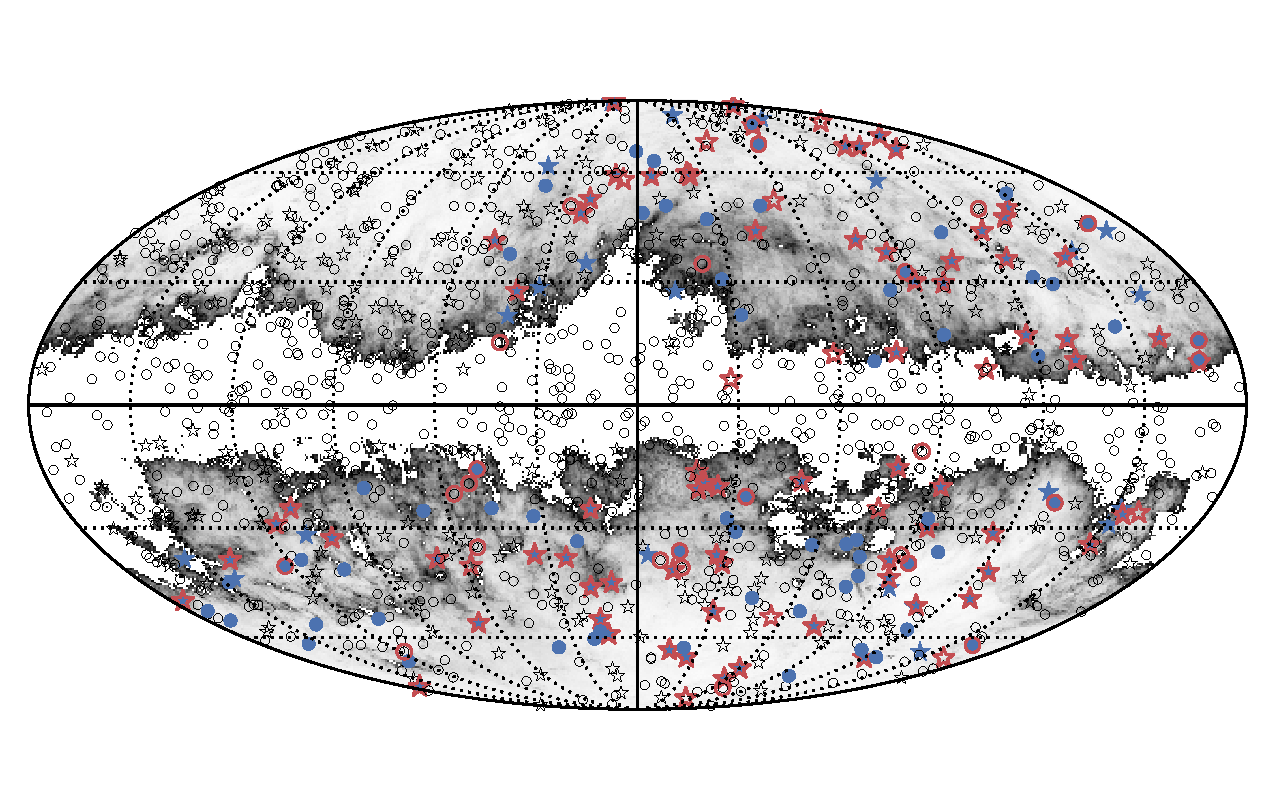
\includegraphics{figures/skymap.pdf}} \caption{Mollweide projection
	in galactic coordinates of the full sky showing the positions on the sky of the
	bursts presented in this work. The equator is the Galactic plane. The empty
	stars/circles are the positions of all the 1266 \textit{Swift} bursts detected
	until \termdate. Stars indicate bursts with measured redshifts and circles
	indicate those without. Blue stars indicate the position of the 98 bursts
	fulfilling the sample criteria specified in Sect. \ref{samplecrit} that have a
	measured redshift. Red outlines are added to the 77 GRBs that enter our
	statistical sample with both X-shooter spectroscopy and a measured redshift.
	Red outlines of empty stars represent bursts which is observed with X-shooter
	and has a measured redshift, but is not a part of our statistical sample. The
	blue dots show the positions of the 63 GRBs of our statistical sample that lack
	redshift measurements. A red outline is added around the 8 bursts in our
	statistical sample which was observed with X-shooter, but did not yield a
	redshift measurement. A single empty circle with a red outline indicate a burst
	outside the statistical sample that was followed up with X-shooter, but without
	a redshift measurement. The different samples are compared in Sect.
	\ref{results}. The background shows the dust maps presented in
	\citet{Schlegel1998}. Please note that we removed the background where the
	sample criteria is violated ($A_V > 0.5$ mag) and replaced it with a white
	color visible at the equator. The grey-scale bar below indicates the value of
	$A_V$ on the plot. The dotted lines indicate intervals of 30$^\circ$ in
	longitude and latitude.} \label{fig:skymap}
\end{figure*}



The observations obtained for this sample have been secured with the
cross-dispersed echelle spectrograph, X-shooter \citep{Vernet2011}, mounted on
one of the two Unit Telescopes at ESO/VLT, UT2 (Kueyen) and UT3 (Melipal) during
the duration of this follow-up campaign. The observations have been taken during
a period of eight years corresponding to the ESO observing periods P84 through P98
under the following programme IDs: 084.A-0260, 085.A-0009, 086.A-0073,
087.A-0055, 088.A-0051, 089.A-0067, 090.A-0088, 0091.C-0934, 092.A-0124,
093.A-0069, 094.A-0134, 095.A-0045, 096.A-0079, 097.A-0036, and 098.A-0055(PI:
Fynbo). These proposals were initiated on Guaranteed Time. We have included a
few additional bursts, from the programmes 084.D-0265 (PI: Benetti), 091.A-0877
(PI: Schady), 092.D-0056 (PI: Rau), 092.D-0633 (PI: Greiner), and 095.B-0811
(PI: Levan). The total collection of spectra represents \textit{all} GRB
afterglows that have been followed up by X-shooter up to \termdate, which marks
the end of the XS-GRB legacy follow-up program.

The first GRB followed up was GRB~090313, observed on the 15th of March, 2009,
during the commissioning of X-shooter on the third Unit Telescope (UT3) of the
VLT . The bursts observed during the commissioning or the science verification
process (GRB~090313, GRB~090530, GRB~090809, GRB~090926) are not a part of the
sample we use to investigate the statistical properties of GRB afterglows, due
to the inhomogeneity of their selection. The first burst observed after science
verification and X-shooter was moved to UT2, was GRB~091018, which is the first
burst entering our statistically homogeneous sample. For all bursts that fulfill
our sample selection criteria, described in Sect. \ref{samplecrit},
spectroscopic follow-up have been attempted with X-shooter. Various conditions
can affect our ability to follow up a given burst, and a discussion of these
conditions and their consequences for the sample is included in Sect.
\ref{badbursts}.

X-shooter covers the spectral wavelength region from 300 nm to 2480 nm in a
single exposure, by separating the light into three separate spectroscopic arms
through the use of two dichroics. The ultraviolet blue (UVB) arm covers 300 -
550 nm, the visual (VIS) arm covers 550 - 1020 nm, and the near-infrared (NIR)
arm covers 1020 - 2480 nm. For some of the observations, we have applied a
$K$-band blocking filter, cutting the coverage of the NIR arm at 2100 nm. This
is done to reduce the amount of scattered background light from the thermal
infrared. For the majority of observations, a nod-and-shuffle observing scheme
has been employed, with a nodding throw of 5\arcsec. Each nodding observation
have typically been carried out in a standard ABBA pattern. For some cases,
conditions during the follow-up, either technical or weather, have necessitated
alterations to this scheme as described in App. \ref{notes}. For RRM triggers, a
slightly different observing strategy was employed. Starting as rapidly as
possible, a simple stare mode sequence was started, with 5 spectroscopic
integrations with increasing exposure times. 

For the majority of the bursts, we have observed with a slit width of 1\farc0,
0\farc9, and 0\farc9 for the UVB, VIS, and NIR-arm respectively. This sets a
lower limit on the delivered resolution of the spectra based on the tabulated
values of the delivered resolutions, which is 4350, 7450, and 5300 for the UVB,
VIS and NIR-arm
respectively\footnote{See \href{https://www.eso.org/sci/facilities/paranal/instruments/xshooter/inst.html}{this URL} for the nominal resolutions.}. %The slit width sets the width of the atmospheric sky lines and determines the amount of light lost due to the wavelength-dependent seeing PSF extending outside the coverage of the slit, where the width of sky-lines is always set by the slit width whereas both the delivered resolution and the slitloss changes for the better as the seeing PSF drops below the slit width. For atmospheric conditions delivering a seeing PSF with a FWHM of 0\farc9 observed with a 0\farc9 slit only 76.1 per cent of the light will enter the slit, meaning that for almost all observations a slitloss correction is required.
%We describe how slitlosses were corrected for in Sect. \ref{postproc}.
For accurate measurements involving line profiles, knowledge of the precise
instrumental resolution is required. The resolution becomes better than the
nominal one, listed above, when the delivered seeing is smaller than the
projected width of the slit on the sky. We discuss how we determine the
effective instrumental resolution in Sect. \ref{resolution}.

Due to a mechanical failure, the atmospheric dispersion corrector (ADC) was
disabled from 1st of August 2012. Only GRB~100728B was affected by the failing
ADC prior to disablement, resulting in a lower-than-nominal throughput. To avoid
chromatic slit losses due to atmospheric dispersion, nearly all subsequent
observations have been carried out at parallactic angle. A consequence of this,
is that for all observations following 1st of August 2012, the centroid of the
trace of the source changes position across the spatial direction of the slit as
a function of wavelength. This effect has been modeled in the extraction
procedure, as described in Sect. \ref{extract}.

\LongTables
	
	\begin{deluxetable*}{@{\extracolsep{\fill}}lcccccclc@{}}
		%\tabletypesize{\scriptsize}
		%\rotate
		\tablecaption{The full sample of afterglows or hosts observed in the program.
			We here list the burst names and details of the spectroscopic observations. The
			exposure times and slit widths are given in the order UVB/VIS/NIR. The column
			$\Delta t$ shows the time after trigger when the spectroscopic observation was
			started. Mag$_\mathrm{acq}$ gives the approximate magnitude (typically in the
			$R$-band) of the afterglow in the acquisition image.
			\label{sample}}
		\tablewidth{0pt}
		\tablehead{
			\colhead{GRB} &  \colhead{Exptime} & \colhead{Slit width} & \colhead{Airmass} & \colhead{Seeing} & \colhead{$\Delta t$} & \colhead{Mag$_\mathrm{acq}$} & \colhead{Redshift} & \colhead{Ref}\\
			&  \colhead{(ks)}   & \colhead{(arcsec)} &   & \colhead{(arcsec)} & \colhead{(hr)}       &  & &  \\
		}
		\startdata
		GRB090313$^1$ 		& 6.9/6.9/6.9     	& 1.0/0.9/0.9 		& 1.2--1.4  	& 1.0  	&    45  	&  21.6  	& 3.3736 		& (1) \\
		GRB090530$^1$ 		& 4.8/4.8/4.8     	& 1.0/1.2/1.2 		& 1.6--2.2  	& 1.5  	&    20  	&  22    	& 1.266 		& (2) \\
		GRB090809$^1$ 		& 7.2/7.2/7.2     	& 1.0/0.9/0.9 		& 1.2--1.1  	& 0.9  	&  10.2  	&  21    	& 2.737  		& (2,3) \\
		GRB090926$^1$ 		& 7.2/7.2/7.2     	& 1.0/0.9/0.9 		& 1.4--1.5  	& 0.9  	&    22  	&  17.9  	& 2.1062 		& (4) \\
		GRB091018     		& 2.4/2.4/2.4     	& 1.0/0.9/0.9 		& 2.1--1.8  	& 0.8  	&   3.5  	&  19.1  	& 0.9710 		& (5) \\  
		GRB091127     		& 6.0/6.0/6.0     	& 1.0/0.9/0.9 		& 1.1--1.2  	& 1.0  	&   101  	&  21.2  	& 0.490  		& (6) \\
		GRB100205A     		& 10.8/10.8/10.8 	& 1.0/0.9/0.9 		& 1.9--1.8  	& 1.0  	&    71  	&   --   	&  --    		& (2) \\
		GRB100219A     		&  4.8/4.8/4.8   	& 1.0/0.9/0.9 		& 1.3--1.1  	& 0.7  	&  12.5  	&   23   	& 4.667  		& (7) \\
		GRB100316B     		&  2.4/2.4/2.4   	& 1.0/0.9/0.9 		& 2.0--2.4  	& 0.7  	&   0.7  	&  18.2  	& 1.18   		& (2) \\
		GRB100316D-1$^2$ 	&  7.2/7.2/7.2   	& 1.0/0.9/0.9 		& 1.2--1.5  	& 1.0  	&  12  		&   --   	& 0.059  		& (8) \\
		GRB100316D-2   		&  2.4/2.4/2.4   	& 1.0/0.9/0.9 		& 1.2--1.2  	& 1.0  	&    58  	&   --   	& 0.059  		& (8) \\
		GRB100316D-3   		&  2.4/2.4/2.4   	& 1.0/0.9/0.9 		& 1.2--1.2  	& 0.8  	&   192  	&   --   	& 0.059  		& (8) \\
		GRB100418A-1   		&  4.8/4.8/4.8   	& 1.0/0.9/0.9 		& 1.6--1.3  	& 0.7  	&   8.4  	&  18.1  	& 0.6235 		& (9) \\
		GRB100418A-2   		&  4.8/4.8/4.8   	& 1.0/0.9/0.9 		& 1.2--1.3  	& 0.6  	&    34  	&  19.2   	& 0.6235 		& (9) \\
		GRB100418A-3   		&  4.8/4.8/4.8   	& 1.0/0.9/0.9 		& 1.2--1.4  	& 0.7  	&    58  	&   --   	& 0.6235 		& (9) \\
		GRB100424A$^3$ 		&  4.8/4.8/4.8   	& 1.0/0.9/0.9 		& 1.1--1.2  	& 0.8  	&   --   	&   --   	& 2.465  		& (2) \\
		GRB100425A     		&  2.4/2.4/2.4   	& 1.0/0.9/0.9 		& 1.5--1.3  	& 0.7  	&   4.0  	&  20.6  	& 1.755  		& (2,3) \\
		GRB100621A     		&  2.4/2.4/2.4   	& 1.0/0.9/0.9 		& 1.3--1.4  	& 1.0  	&   7.1  	&   --   	& 0.542  		& (2) \\
		GRB100625A$^3$ 		&  4.8/4.8/4.8   	& 1.0/0.9/0.9 		& 1.1--1.0  	& 0.8  	&    13  	&   --   	& 0.452  		& (2) \\
		GRB100724A$^4$ 		&  4.2/4.2/4.2   	& 1.0/0.9/0.9 		& 1.5--2.3  	& 0.7  	&   0.2  	&   --   	& 1.288  		& (2) \\
		GRB100728B$^5$ 		&  7.2/7.2/7.2   	& 1.0/0.9/0.9 		& 1.5--1.1  	& 0.5  	&    22  	&   23   	& 2.106  		& (2) \\
		GRB100814A-1$^4$ 	& 0.9/0.9/0.9  		& 1.0/0.9/0.9 		& 1.9--1.7  	& 0.5  	&   0.8  	&   19   	& 1.44   		& (2) \\
		GRB100814A-2   		&  4.8/4.8/4.8   	& 1.0/0.9/0.9 		& 1.5--1.2  	& 0.6  	&   1.4  	&   19   	& 1.44   		& (2) \\
		GRB100814A-3   		&  4.8/4.8/4.8   	& 1.0/0.9/0.9 		& 1.2--1.0  	& 0.6  	&   99   	&   20   	& 1.44   		& (2) \\
		GRB100816A$^6$ 		&  4.8/4.8/4.8   	& 1.0/0.9/0.9 		& 1.8--1.6  	& 0.8  	&   3.7  	&   --   	& 0.806  		& (2) \\
		GRB100901A     		&  2.4/2.4/2.4   	& 1.0/0.9/0.9 		& 1.5--1.5  	& 1.8  	&   66   	&   --   	& 1.408  		& (10) \\
		GRB101219A     		&  7.2/7.2/7.2   	& 1.0/0.9/0.9 		& 1.1--1.7  	& 2.0  	&   3.7  	&   --   	& 0.718  		& (2) \\
		GRB101219B-1   		&  4.8/4.8/4.8   	& 1.0/0.9/0.9 		& 1.6--2.6  	& 1.3  	&  11.6  	&   20   	& 0.5519 		& (11) \\
		GRB101219B-2   		&  7.2/7.2/7.2   	& 1.0/0.9/0.9 		& 1.2--2.0  	& 0.8  	&   394  	&  22.7  	& 0.5519 		& (11) \\
		GRB101219B-3   		&  7.2/7.2/7.2   	& 1.0/0.9/0.9 		& 1.4--2.1  	& 0.9  	&   886  	&   --   	& 0.5519 		& (11) \\
		GRB110128A     		&  7.2/7.2/7.2   	& 1.0/0.9/0.9 		& 2.0--1.6  	& 0.9  	&   5.5  	&  22.5  	& 2.339  		& (2) \\
		GRB110407A     		&  9.6/9.6/9.6   	& 1.0/0.9/0.9 		& 1.4--1.3  	& 2.0  	&  12.4  	&   23   	&  --    		& (2) \\
		GRB110709B$^1,3$ 	&  7.2/7.2/7.2 		& 1.0/0.9/0.9 		& 1.6--1.1  	& 1.0  	&   --   	&   --   	&  --    		& (2) \\
		GRB110715A     		&  0.6/0.6/0.6   	& 1.0/0.9/0.9 		& 1.1--1.1  	& 1.7  	&  12.3  	&  18.5  	& 0.82  		& (2) \\
		GRB%110721A     	&  2.4/2.4/2.4   	& 1.0/0.9/0.9 		& 1.2--1.4  	& 2.4  	&        	&        	& 0.382  		& (2) \\
		GRB110808A     		& 2.4/2.4/2.4    	& 1.0/0.9/0.9 		& 1.2--1.1  	& 1.1  	&   3.0  	&  21.2  	& 1.3488 		& (2) \\
		GRB110818A     		& 4.8/4.8/4.8    	& 1.0/0.9/0.9 		& 1.3--1.3  	& 1.0  	&   6.2  	&  22.3  	& 3.36   		& (2) \\
		GRB111005A$^3$ 		& 1.2/1.2/1.2    	& 1.0/0.9/0.9 		& 1.3--1.3  	& 0.7  	&   --   	&  --    	& 0.013? 		& (2) \\
		GRB111008A-1   		& 8.8/8.8/8.4    	& 1.0/0.9/0.9 		& 1.1--1.0  	& 1.2  	&   8.5  	&  21?   	& 4.9898 		& (12) \\
		GRB111008A-2   		& 8.0/8.0/7.2    	& 1.0/0.9/0.9 		& 1.3--1.0  	& 1.0  	&  20.1  	&  22?   	& 4.9898 		& (12) \\
		GRB111107A     		& 4.8/4.8/4.8    	& 1.0/0.9/0.9 		& 1.8--1.5  	& 0.7  	&   5.3  	&  21.5  	& 2.893  		& (2) \\
		GRB111117A$^6$ 		& 4.8/4.8/4.8    	& 1.0/0.9/0.9 		& 1.5--1.4  	& 0.6  	&    38  	&  --    	& 1.3?   		& (2) \\
		GRB111123A-1   		& 6.2/6.6/6.6    	& 1.0/0.9/0.9 		& 1.6--1.1  	& 1.0  	&  12.2  	&  $>$24 	& 3.1516 		& (2) \\
		GRB111123A-2$^3$ 	& 2.4/2.4/2.4  		& 1.0/0.9/0.9 		& 1.0--1.0  	& 0.5  	&   --   	&  --    	& 3.1516 		& (2) \\
		GRB111129A     		& 3.6/3.6/3.6    	& 1.0/0.9/0.9 		& 1.6--2.1  	& 1.7  	&        	&        	&  --    		& (2) \\
		GRB111209A-1   		& 4.8/4.8/4.8    	& 1.0/0.9/0.9 		& 1.1--1.2  	& 0.8  	&  17.7  	&  20.1  	& 0.677  		& (13) \\
		GRB111209A-2   		& 9.6/9.6/9.6    	& 1.0/0.9/0.9 		& 1.2--2.0  	& 0.8  	&  497   	&  23    	& 0.677  		& (13) \\
		GRB111211A$^1$ 		& 2.4/2.4/2.4    	& 1.0/0.9/0.9 		& 1.4--1.6  	& 0.6  	&   31   	&  19.5  	& 0.478  		& (2) \\
		GRB111228A     		& 2.4/2.4/2.4    	& 1.0/0.9/0.9 		& 1.4--1.4  	& 0.9  	&  15.9  	&  20.1  	& 0.716  		& (2) \\
		GRB120118B$^3$ 		& 3.6/3.6/3.6    	& 1.0/0.9/0.9 		& 1.1--1.0  	& 1.0  	&   --   	&  --    	& 2.943  		& (2) \\
		GRB120119A-1   		& 2.4/2.4/2.4    	& 1.0/0.9/0.9 		& 1.1--1.1  	& 0.6  	&   1.4  	&   17   	& 1.728  		& (2) \\
		GRB120119A-2   		& 1.2/1.2/1.2    	& 1.0/0.9/0.9 		& 1.8--1.9  	& 0.6  	&   4.5  	&   20   	& 1.728  		& (2) \\
		GRB120119A-3$^3$ 	& 4.8/4.8/4.8  		& 1.0/0.9/0.6JH 	& 1.0--1.1  	& 1.1 	&   --   	&   --   	& 1.728  		& (2) \\
		GRB120211      		&                	&             		&           	&      	&        	&         	& 2.346 		& (2) \\
		GRB120224A     		& 2.4/2.4/2.4    	& 1.0/0.9/0.9 		& 1.7--2.1  	& 1.4  	&  19.8  	&   22.3 	&  --    		& (2) \\
		GRB120311A     		& 2.4/2.4/2.4    	& 1.0/0.9/0.9 		& 1.6--1.4  	& 0.6  	&   3.7  	&   21.6 	&  --    		& (2) \\
		GRB120327A-1   		& 2.4/2.4/2.4    	& 1.0/0.9/0.9 		& 1.6--1.4  	& 0.5  	&   2.1  	&   18.8 	& 2.815  		& (14) \\
		GRB120327A-2   		& 4.2/4.2/4.2    	& 1.0/0.9/0.9 		& 1.0--1.1  	& 1.0  	&    29  	&   22.5 	& 2.815  		& (14) \\
		GRB120404A     		& 9.6/9.6/9.6    	& 1.0/0.9/0.9JH 	& 1.7--1.3 		& 1.3 	&  15.7  	&   21.3 	& 2.876  		& (2) \\
		GRB120422A-1   		& 4.8/4.8/4.8    	& 1.0/0.9/0.9 		& 1.3--1.3  	& 0.6  	&  17.2  	&   22.0 	& 0.283  		& (15) \\
		GRB120422A-2   		& 4.8/4.8/4.8    	& 1.0/0.9/0.9 		& 1.3--1.4  	& 0.9  	&  113   	&   --   	& 0.283  		& (15) \\
		GRB120422A-3   		& 4.8/4.8/4.8    	& 1.0/0.9/0.9 		& 1.4--1.7  	& 1.0  	&  210   	&   --   	& 0.283  		& (15) \\
		GRB120422A-4   		& 4.8/4.8/4.8    	& 1.0/0.9/0.9JH 	& 1.3--1.4 		& 0.6  	& 449   	&   --   	& 0.283  		& (15) \\
		GRB120422A-5   		& 4.8/4.8/4.8    	& 1.0/0.9/0.9JH 	& 1.3--1.6 		& 0.8  	& 593   	&   --   	& 0.283  		& (15) \\
		GRB120422A-6   		& 4.8/4.8/4.8    	& 1.0/0.9/0.9JH 	& 1.7--2.4 		& 2.5  	& 882   	&   --   	& 0.283  		& (15) \\
		GRB120422A-7   		& 4.8/4.8/4.8    	& 1.0/0.9/0.9JH 	& 1.5--1.9 		& 1.3  	& 906   	&   --   	& 0.283  		& (15) \\
		GRB120712A     		& 4.8/4.8/4.8    	& 1.0/0.9/0.9   	& 1.5--2.5 		& 1.3  	& 10.4  	&   21.5 	& 4.175  		& (2) \\
		GRB120714B     		& 4.8/4.8/4.8    	& 1.0/0.9/0.9JH 	& 1.5--1.2 		& 1.2  	&  7.8  	&   22.1 	& 0.398  		& (2)\\
		GRB120716A$^1$ 		& 3.6/3.6/3.6    	& 1.0/0.9/0.9JH 	& 1.8--2.6 		& 1.0  	&  62   	&   20.9 	& 2.486  		& (2) \\
		GRB120722A$^2$ 		& 4.8/4.8/4.8    	& 1.0/0.9/0.9   	& 1.3--1.3 		& 1.1  	& 10.3  	&   23.6 	& 0.959  		& (2) \\
		GRB120805A$^2$ 		& 3.6/3.6/3.6    	& 1.0/0.9/0.9JH 	& 1.3--1.7 		& 0.9  	& 218   	&   --   	& 2.8?   		& (2) \\
		GRB120815A     		& 2.4/2.4/2.4    	& 1.0/0.9/0.9   	& 1.3--1.4 		& 0.6  	&  1.7  	&   20   	& 2.358  		& (16) \\
		GRB120909A     		& 1.2/1.2/1.2    	& 1.0/0.9/0.9   	& 1.6--1.6 		& 1.4  	&  1.7  	&   21   	& 3.929  		& (2) \\
		GRB120923A     		& 9.6/9.6/9.6    	& 1.0/0.9/0.9JH 	& 1.2--1.4 		& 1.0  	& 18.5  	&   --   	& $\gtrsim8$ 	& (2) \\
		GRB121024A     		& 2.4/2.4/2.4    	& 1.0/0.9/0.9   	& 1.2--1.1 		& 0.6  	&  1.8  	&   20   	& 2.300  		& (17) \\
		GRB121027A     		& 8.4/8.4/8.4    	& 1.0/0.9/0.9   	& 1.3--1.3 		& 0.9  	&  69   	&  21.1  	& 1.773  		& (2) \\
		GRB121201A     		& 4.8/4.8/4.8    	& 1.0/0.9/0.9JH 	& 1.1--1.1 		& 0.9  	& 12.9  	&   23   	& 3.385  		& (2) \\
		GRB121229A     		& 4.8/4.8/4.8    	& 1.0/0.9/0.9JH 	& 1.4--1.2 		& 1.4  	&  2.0  	&  21.5  	& 2.707  		& (2) \\
		GRB130131B$^3$ 		& 7.2/7.2/7.2    	& 1.0/0.9/0.9JH 	& 1.3--1.6 		& 0.8  	&  --   	&   --   	& 2.539  		& (2) \\
		GRB130408A     		& 1.2/1.2/1.2    	& 1.0/0.9/0.9   	& 1.0--1.0 		& 1.0  	&  1.9  	&   20   	& 3.758  		& (2) \\
		GRB130418A     		& 1.2/1.2/1.2    	& 1.0/0.9/0.9   	& 1.4--1.3 		& 1.3  	&  4.6  	&   18.5 	& 1.218  		& (2) \\
		GRB130427A     		& 1.2/1.2/1.2    	& 1.0/0.9/0.9JH 	& 1.8--1.8 		& 0.8  	& 16.5  	&   19   	& 0.340  		& (18) \\
		GRB130427B     		& 1.2/1.2/1.2    	& 1.0/0.9/0.9JH 	& 1.2--1.0 		& 0.8  	& 20.3  	&   22.7 	& 2.78   		&  (2) \\
		GRB130603B$^6$ 		& 2.4/2.4/2.4    	& 1.0/0.9/0.9   	& 1.4--1.4 		& 1.1  	&  8.2  	&   21.5 	& 0.356  		& (19) \\
		GRB130606A     		& 4.2/4.2/4.2    	& 1.0/0.9/0.9JH 	& 1.7--1.9 		& 1.1  	&  7.1  	&   19   	& 5.91   		& (20) \\
		GRB130612A     		& 1.2/1.2/1.2    	& 1.0/0.9/0.9   	& 1.3--1.3 		& 1.4  	&  1.1  	&   21.5 	& 2.006  		& (2) \\
		GRB130615A     		& 1.2/1.2/1.2    	& 1.0/0.9/0.9   	& 2.1--2.2 		& 1.0  	&  0.8  	&   21   	& $~3$?  		& (2) \\
		GRB130701A     		& 1.2/1.2/1.2    	& 1.0/0.9/0.9JH 	& 2.0--2.0 		& 1.6  	&  5.5  	&   19.9 	& 1.155  		& (2) \\
		\enddata
		\tablenotetext{1}{Not part of the statistical sample}
		\tablenotetext{2}{Spectrum dominated by light from the host galaxy}
		\tablenotetext{3}{Spectrum of the host galaxy taken long after the burst}
		\tablenotetext{4}{RRM observation}
		\tablenotetext{5}{ADC malfunction during observation}
		\tablenotetext{6}{Short burst}
		\tablerefs{
			(1) \citet{DeUgartePostigo2010}; (2) This work ; (3) Skuladottir (2010);
			(4) \citet{DElia2010}; (5) \citet{Wiersema2012}; (6) \citet{Vergani2011, Cobb2010}; 
			(7) \citet{Thone2013}; (8) \citet{Bufano2012} ; (9) \citet{DeUgartePostigo2011} ;
			(10) \citet{Hartoog2013}; (11) \citet{Sparre2011}; (12) \citet{Sparre2014};
			(13) \citet{Levan2014}; (14) \citet{DElia2014}; (15) \citet{Schulze2014};
			(16) \citet{Kruhler2013}; (17} \citet{Friis2015}
	\end{deluxetable*}
	%-------------------------END TABLE---------------------------------------
	

We provide an overview of all the observations in Table
\ref{tab:sample_overview} and plot the positions of all the bursts on the
celestial sphere in galactic coordinates in Fig. \ref{fig:skymap}. Away from the
central zone of avoidance, due to high Galactic extinction cutoff (marked in
white), the GRB positions have an isotropic distribution, except in the upper
left quadrant which cannot be observed from Paranal.

30 percent of the spectra presented here, primarily host observations, have
already been published in \citet{Kruhler2015}. Single bursts have additionally
been published, based on unusual properties in their afterglows. We present
individual notes on all the X-shooter spectra and their previous use in App.
\ref{notes}. We include independent reductions of them here for completeness.

%%%%%%%%%%%%%%%%%%%%%%%%%%%%%%%%%%%%%%%%%%%%%%%%%%%%%%%%%%%%%%%%%%%%%%%%%%%%
\section{Data processing} \label{proc}
%%%%%%%%%%%%%%%%%%%%%%%%%%%%%%%%%%%%%%%%%%%%%%%%%%%%%%%%%%%%%%%%%%%%%%%%%%%%

In this section we describe how the final data products are produced and
subsequently post-processed. 
%29 percent of the data released here have been
% reduced in a manner similar to what is described in \citet{Kruhler2015}.
% The two reduction schemes have been tested and are in good agreement.
All post-processing scripts developed for this dataset are made publicly
available at \url{https://github.com/jselsing/XSGRB_reduction_scripts}.

Before any reductions are initiated, the raw object images are run through the
cosmic-ray removal algorithm \citep{VanDokkum2001} implementation,
\textit{Astro-SCRAPPY}\footnote{\url{https://github.com/astropy/astroscrappy}},
where a wide clipping radius was used around detected cosmic ray hits to ensure
that edge residuals are robustly rejected.

The basis for the reductions is the VLT/X-shooter pipeline, version
\texttt{2.7.1} or newer \citep{Goldoni2006, Modigliani2010}. The pipeline is
managed with the Reflex interface \citep{Freudling2013} and is used for
subtraction of bias level, flat-fielding, tracing of the echelle orders,
wavelength calibrations with the use of arc-line lamps, flux calibration using
spectrophotometric standards \citep{Vernet2010, Hamuy1994}, mirror flexure
compensation(see Sect. \ref{wavecal}), sky-subtraction and lastly the
rectification and merging of the orders. Errors and bad pixel maps are
propagated throughout the extraction. For the initial sky-subtraction, the
background has been estimated by a running median in regions adjacent to the
object trace clear of contaminating sources. Due to the broken ADC, for some
objects there is curvature in the object trace along the dispersion axis of the
slit(see Sect. \ref{extract}). This means that for these bursts, the initial
sky-estimate was made from a limited number of pixels in the spatial direction.
The subtraction of the sky background on the un-rectified image ensures that the
bulk of the sky background is not redistributed by the rectification process.

X-shooter is an echelle spectrograph, and therefore the individual echelle
orders are curved across image space. The individual orders therefore need to be
rectified. In order to transform the image space (pixels) into a physical
(wavelength-slit) space, the image pixels are resampled onto a physical grid,
while propagating the pixel uncertainties derived by the pipeline. This
rectification  process correlates neighboring pixels and in order to minimize
the degree of correlation, we need to choose a physical sampling that matches
the pixel sampling. We rectified the image onto an equidistant grid with a
dispersion sampling of 0.02 nm/pixel and a 0\farcs16 per pixel spatial sampling
for the UVB and VIS arm and 0.06 nm/pixel with a 0\farcs21 per pixel in the NIR
arm.  Because the tabulated resolution is a lower limit to the delivered
resolution, we choose a sampling of 0.02 nm/pixel to ensure that the lowest
wavelength part of neither of the arms have a sampling lower than the Nyquist
sampling rate of 2 pixels per resolution FWHM.

%%%%%%%%%%%%%%%%%%%%%%%%%%%%%%%%%%%%%%%%%%%%%%%%%%%%%%%%%%%%%%%%%%%%%%%%%%%%
\subsection{Post-processing} \label{postproc}
%%%%%%%%%%%%%%%%%%%%%%%%%%%%%%%%%%%%%%%%%%%%%%%%%%%%%%%%%%%%%%%%%%%%%%%%%%%%

For a typical observation, each of the exposures in the nodding sequence has
been reduced as a single observation and then subsequently combined to form a
single image. We employ this strategy so that we can reject outliers in the
stack and weight by an averaged measure of the inverse variance of the
background. When weighting images, where the noise in each pixel is dominated by
Poisson noise, it is important to estimate the background variance in a large
enough region, so that any correlation between the signal and the weights are
removed. To this end, the weight map is generated by a running median window
over the variance map produced by the pipeline, where the trace has been masked
and the width of the window is chosen to be wide enough for the median variance to
be calculated on the basis of several hundred pixels. This weighting scheme
automatically also optimally combines images of different exposure times or
images where the background is varying, which is often the case when a burst has
been observed close to twilight

An additional sky-subtraction is additionally run on all rectified 2D spectra.
This is done to remove residual sky, still present. At each pixel in the
dispersion direction, the spatial dimension is fit with a low-order polynomial,
after all sources are masked out. This low order polynomial is then convolved
with a few pixel wide Gaussian filter in the dispersion direction and subtracted
of the entire 2D image.

In the NIR arm where the background is very bright and there are a high number
of broad sky-lines, an alternative approach to sky subtraction has been
employed. When there are no contaminating sources in the slit, the sky has been
put back on the images and the images are combined in pairs of two, subtracting
the two from each other while keeping the WCS static. Due to the nod-and-shuffle
offsets used between observations, this conserves the source flux while removing
the sky at the expense of a decrease in signal-to-noise by a factor of
$\sqrt{2}$. This amounts to the regular nodding reduction, only we can reject
outliers and weight by the averaged inverse variance map.

Reducing the images as single observations for all exposures, we additionally
get a spectrum of the sky which we can use to recalibrate the wavelength
solution.


%%%%%%%%%%%%%%%%%%%%%%%%%%%%%%%%%%%%%%%%%%%%%%%%%%%%%%%%%%%%%%%%%%%%%%%%%%%%
\subsection{Correction for offsets in the wavelength calibration}    \label{wavecal}
%%%%%%%%%%%%%%%%%%%%%%%%%%%%%%%%%%%%%%%%%%%%%%%%%%%%%%%%%%%%%%%%%%%%%%%%%%%%

Since X-shooter is installed at the VLT Cassegrain focus, it is prone to
flexures. The flexures modify the projection of the slit on the detector with
respect to the one obtained in daytime calibration. This requires a modification
of the wavelength solution in order to correctly process the night-time data.
Part of this correction is performed by the pipeline using the frames taken
during the X-shooter Active Flexure Compensation procedure\footnote{X-shooter
	User Manual available at \href{https://www.eso.org/sci/facilities/paranal/instruments/xshooter/doc.html}{ESO website}}. The
remaining offset is corrected by cross-correlating the observed sky spectrum
with a synthetic sky spectrum \citep{Noll2012, Jones2013} after the continuum,
estimated as the mode of all flux values, has been subtracted. To get the
correct seeing point-spread-function (PSF) with which to convolve the synthetic sky, an initial
refinement of the wavelength solution has been obtained by cross-correlating the
observed sky with an unconvolved synthetic sky. This preliminary wavelength
calibration is applied to the observed sky. The synthetic spectrum is then
convolved with an increasing seeing PSF and the width that minimizes $\chi^2$
with the updated observed sky is chosen to be the effective sky-PSF. Using the
synthetic sky with the matched resolution, a final wavelength calibration can
then be calculated by cross-correlating the observed sky with the correctly
broadened sky spectrum as a function of a velocity offset. Both a
multiplicative and an additive offset to the wavelength calibration has been
tested, but in terms of $\chi^2$, the model with only a multiplicative offset is
preferred. The resulting offsets, which were smaller than 0.01 nm in the UVB and
VIS data and smaller than 0.05 nm in the NIR spectra, but changing over short
periods of time were applied to the corresponding spectra\footnote{The
	wavelength shifts have been extensively studied by
	ESO \href{https://www.eso.org/sci/facilities/paranal/instruments/xshooter/doc/XS_wlc_shift_150615.pdf}{in this document}.}. Using the convolved synthetic sky, the pixels containing the brightest sky lines have been added to the bad pixel map.

%%%%%%%%%%%%%%%%%%%%%%%%%%%%%%%%%%%%%%%%%%%%%%%%%%%%%%%%%%%%%%%%%%%%%%%%%%%%
\subsection{Spectral extraction}    \label{extract}
%%%%%%%%%%%%%%%%%%%%%%%%%%%%%%%%%%%%%%%%%%%%%%%%%%%%%%%%%%%%%%%%%%%%%%%%%%%%

To extract the afterglow spectrum from the rectified 2D-image, several
techniques have been employed based on the brightness of the afterglow and the
complexity of the objects entering the slit. Due to the malfunctioning ADC, see
Sect. \ref{obs}, the spectral trace changes position across the slit in the
spatial direction as a function of wavelength. For a large fraction of the
observed bursts, using a single aperture for the spectral extraction is
inadequate due to the large amount of background that would then enter the slit.
To optimally select the extraction regions we therefore need to model the trace
position.

To get the shape and the position of the spectral PSF as a function of location
on the image, we need to chose a model which can represent how the light falls
on the slit. We know from \citet{Trujillo2001} that a Moffat function
\citep{Moffat1969} with an index of $\beta = 4.765$ adequately describes an
imaging PSF due to atmospheric turbulence, but because of aberrations in the
dispersion elements and the rectification process, the PSF we are trying to
model is different from this profile. To allow for flexibility in the model, we
have chosen the Voigt function as a model for the spectral PSF and we describe
how this is evaluated in App. \ref{voigt}. Since the host galaxy could also give
a contribution to the image profile, this choice allows for the required freedom
if additional flux is in the wings of the profile.

To guide the estimated position of the trace on the slit as a function of
wavelength, we have used the analytic prescription for the trace position
described in \citet{Filippenko1982}, where the header keywords of the
observations have been queried for the ambient conditions which controls the
degree to which the trace changes position in the spatial direction.

Based on the signal-to-noise of the afterglow continuum, the 2D-image has been
binned down in the spectral direction to a number of elements that allows for an
accurate tracing of the PSF, typically 200 bins for moderate signal-to-noise.
For each of the bins, using the analytically guided guess position, the spectral
PSF has been fit using the unweighted chi-squared minimization algorithm
implemented in \texttt{scipy.optimize.curve\_fit} \citep{scipy}. Since we know
that the trace varies slowly as a function of wavelength, we have then fitted a
low-order polynomial to the fit parameters as a function of wavelength, which
allows us to evaluate the spectral PSF at all wavelengths and in this way
accurately model the entire spectral PSF.

Equipped with a model for how the light is distributed across the entire
dispersion direction, we can  employ the optimal extraction algorithm
\citep{Horne1986}, which weights the extraction aperture by the spectral profile,
or alternatively sum all pixels within 1 FWHM of the modeled profile. Where
possible, we have used the optimal extraction. In cases where the trace is very
weak, even in the binned images, an aperture has been selected manually which
covers all emission lines, if present, and when nothing is immediately visible, the
entire nodding window. The error- and bad pixel maps are in all cases propagated
throughout the extraction.

In cases where multiple traces are visible in the slit, additional components
for the profile are used in the optimal extraction. The additional components do
not share the PSF parameters and in cases where the additional component is an
extended object, the fits have been inspected to ensure that the additional
component does now skew the fit towards a different PSF. The additional
components are not used for the weights in the extractions.

The spectra are corrected for Galactic extinction using the $E(B-V)$ value from
the dust maps of \citet{Schlegel1998} with the update in
\citet{Schlafly2011}\footnote{Queried from
	http://irsa.ipac.caltech.edu/applications/DUST/index.html using \texttt{astroquery}
	\citep{astroquery}.}, and the extinction curve by \cite{Cardelli1989} with a
total to selective extinction $R_V = 3.1$. The wavelengths of the extracted
1D-spectra are moved to vacuum, corrected for barycentric motion, and the
wavelength recalibration described in Sect. \ref{wavecal} is applied. Pixels
with pixel-to-pixel variation larger than $50 \sigma$ are additionally added to
the bad pixel map.


%%%%%%%%%%%%%%%%%%%%%%%%%%%%%%%%%%%%%%%%%%%%%%%%%%%%%%%%%%%%%%%%%%%%%%%%%%%%
\subsection{Telluric correction} \label{tell_corr}
%%%%%%%%%%%%%%%%%%%%%%%%%%%%%%%%%%%%%%%%%%%%%%%%%%%%%%%%%%%%%%%%%%%%%%%%%%%%

For all earth-based telescopes, the light first has to pass through Earths
atmosphere, where the atmospheric content and conditions make an imprint on the
received spectrum. These telluric features can be corrected for in a multitude
of ways. We employ a prioritized list of methods here, depending on the
availability of the chosen methods. Since the observations are often taken at
odd times under varying conditions, this prioritized list ensures that we are
always doing the best possible correction.

The highest priority method is using the GRB afterglow continuum itself, where
the atmospheric conditions have directly been imprinted on the spectrum. The
telluric features can directly be fit with an atmospheric model
(\texttt{Molecfit} \citep{Smette2015,
	Kausch2015}\footnote{\url{http://www.eso.org/sci/software/pipelines/skytools/molecfit}}), which can then be used to correct for the absorption. The accuracy of the correction depends on the signal-to-noise per pixel of the target spectrum, where we have chosen the requirement that the afterglow continuum spectrum has a median signal-to-noise higher than a value of 10.

If the afterglow is not sufficiently bright, telluric standard stars observed
close in time to the GRB can be used as a proxy for the atmospheric
condition during the GRB observation. Here we employ the telluric correction
method that has been developed in \citet{Selsing2015}, where a library of
synthetic templates is fit to the observed telluric standard.

In the last case, where the object is neither bright enough, or there for some
reason have not been observed a telluric standard, we rely on a synthetic sky
model \citep{Noll2012, Jones2013} for which we generate a
synthetic transmission spectrum, where the ambient parameters for the
observations have been used.


\begin{figure*}
	\centerline{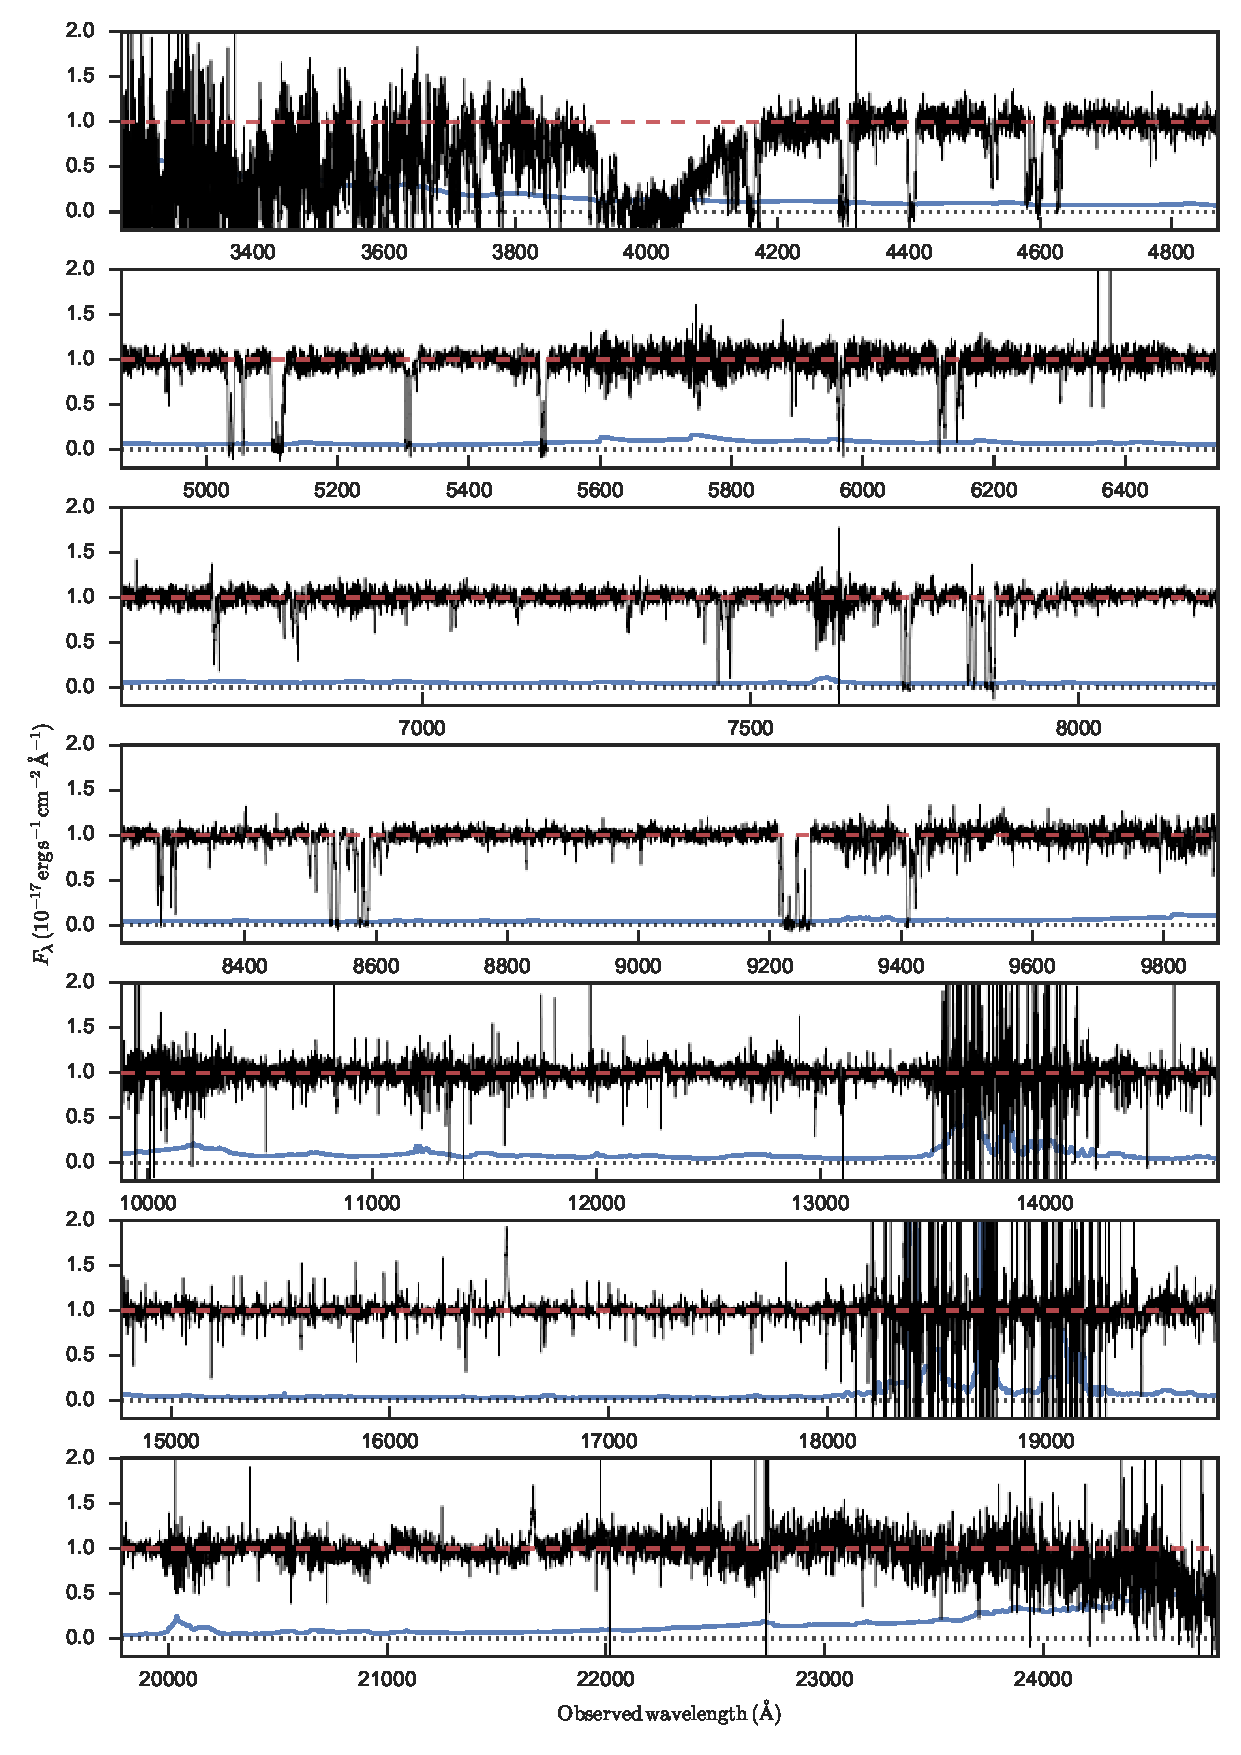
\includegraphics[width=0.85\linewidth]{figures/GRB121024A.pdf}}
\caption{Telluric corrected, normalized spectrum of GRB~121024A at $z = 2.300$,
	that illustrates the typical data quality. The continuum estimate is shown in
	dashed red and the error spectrum in solid blue. The acquisition magnitude is
	$r$ = 20, meaning it is in the brighter end of the sample presented here, but
	not the brightest. The spectrum is rich in absorption and emission, including
	absorption from molecular $\mathrm{H_2}$. The absorption trough visible at
	$\sim$ 4000 $\AA$ is due to \lya~in the host. We have marked the most prominent
	lines seen in GRB afterglows from \citet{Christensen2011a}. The regions of most
	severe telluric absorption is highlighted by a grey-shading the background.
	Additionally, three intervening systems are seen in this sightline. This
	spectrum has been analyzed in detail in \citet{Friis2015}.}
\label{fig:spectrum}
\end{figure*}



%%%%%%%%%%%%%%%%%%%%%%%%%%%%%%%%%%%%%%%%%%%%%%%%%%%%%%%%%%%%%%%%%%%%%%%%%%%%
\subsection{Continuum estimate} \label{continuum}
%%%%%%%%%%%%%%%%%%%%%%%%%%%%%%%%%%%%%%%%%%%%%%%%%%%%%%%%%%%%%%%%%%%%%%%%%%%%

We additionally provide an estimate of the continuum for all the spectra
presented here. For this, we have developed an algorithmic approach that
attempts to automatically estimate the continuum placement along with the error
on the continuum estimate through an iterative procedure. The method is entirely
data-driven and does not rely on any physical assumptions. The method is applied
on each arm separately for each spectrum, to allow the widest possible
wavelength range of the spectral shape to guide the normalization.

To estimate the continuum, a number of points (typically on the order of 100)
are inserted at random positions along the wavelength direction, and the
flux-density of each point is determined by the median value of the spectrum in
a small region ($\sim 1~\mathrm{\AA}$) surrounding each point. The points are
fitted with a low order polynomial (we use \texttt{numpy.polynomial.chebyshev})
and iteratively, the point furthest away is removed until the polynomial fit
differed from the points by less than $\sim$ 5 per cent. This filtering is used
because the intrinsic afterglow continuum of GRBs can be modeled by power laws
\citep{Piran2005}, and removing points that differ significantly from a smooth
continuum shape will guide the continuum estimate to a shape more reasonable for
GRB afterglows. The reason for the non-physical model for the normalization is
that it has the flexibility to captures instrumental variations of the continuum
level that are not easily contained in a more physically motivated model.
Additionally, points spaced closer than 1 per cent of the total spectral
coverage are pruned. The remaining filtered and pruned points are then spline
interpolated using \texttt{scipy.interpolate.splrep.splev}, which serves as a
first estimate of the continuum placement. To avoid the spline to diverge at the
edges, the spline-based continuum is tapered with a low order polynomial. An
attempt to identify absorption and emission regions are then carried out, where
they are marked as such if the difference between the estimated continuum and
the observed spectrum is larger than 3 - 5 times the associated error spectrum.
All regions marked as affected are then masked.

Using the masked spectrum, the entire process is then repeated 500 times where
the final continuum estimate is the mean of the continuum realizations and the
associated error estimate is the standard deviation. This error reflects the
stability of the algorithm across the spectrum. An example of the performance is
shown in Fig. \ref{fig:spectrum}. In the \lya~forest, where there is very little
flux at the continuum level, the performance of the normalization algorithm
depends on the continuum coverage redwards of the \lya~line. In some cases, very
little continuum is contained in a single arm and a manual continuum estimate is
provided, similar to what is done in \citet{Lopez2016}. In these cases the
continuum error is set to 10 per cent. The code for the continuum estimate is
released along with the paper at
\url{https://github.com/jselsing/XSGRB-sample-paper}.
                                                                                           
%%%%%%%%%%%%%%%%%%%%%%%%%%%%%%%%%%%%%%%%%%%%%%%%%%%%%%%%%%%%%%%%%%%%%%%%%%%%
\subsection{Spectral resolution} \label{resolution}
%%%%%%%%%%%%%%%%%%%%%%%%%%%%%%%%%%%%%%%%%%%%%%%%%%%%%%%%%%%%%%%%%%%%%%%%%%%%


\begin{figure}[!ht]
	\centerline{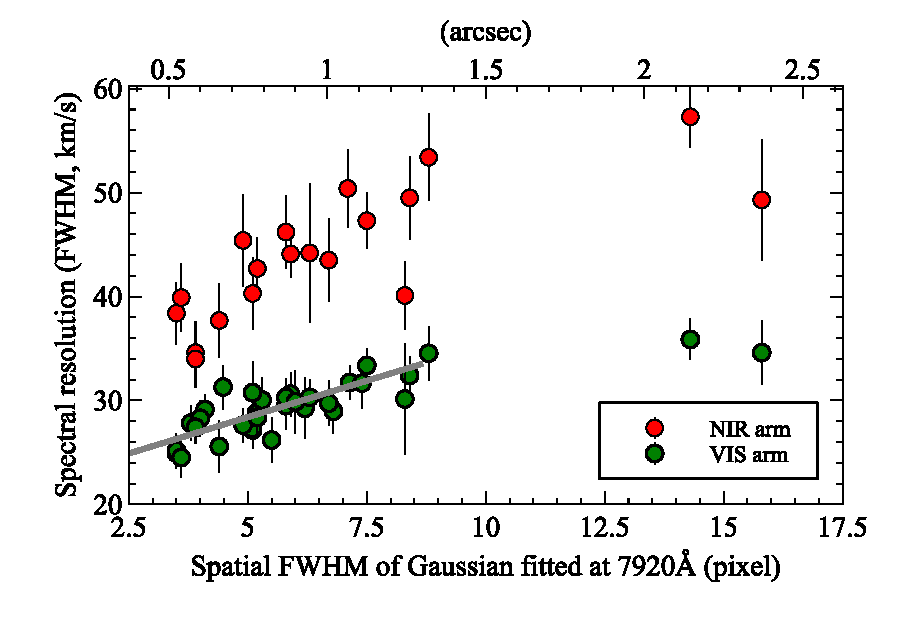
\includegraphics[width=8cm]{figures/resolution_paper.eps}}
\caption{Green datapoints show the FWHM (km/s) of Gaussian fits to unresolved
	telluric absorption lines in the VIS spectra, as a function of the FWHM of a
	Gaussian fit onto the trace in the spatial direction at 792 nm. The lower
	horizontal axis is in units pixels, the top axis in arc seconds. The red
	datapoints show a subsample of measurements obtained for NIR spectra. The grey
	line shows a linear fit to the VIS datapoints. } \label{fig:res}
\end{figure}


The afterglow spectra described in this paper are obtained in
Target-of-Opportunity (override) mode. In most cases, there is little
possibility to tweak slit widths to the seeing at the time of observations (i.e.
to optimize spectral resolution and signal-to-noise), and almost all our data are
therefore taken with a fixed set of slit widths and binning, described above. In
a fair number of cases, the seeing full width at half maximum (FWHM) is
considerably smaller than the slit width, and the delivered spectral resolution
will then be determined by the seeing rather than by the slit width, as afterglows are
point sources (this is evidently not the case for extended sources, e.g for host
galaxies). The delivered resolution for slit-width dominated spectra
post-reduction and extraction can easily be determined from the bright sky
emission lines. For afterglow spectra with very high signal-to-noise, the
delivered spectral resolution can at times be determined from the science data
themselves. However, in the presence of multiple velocity components in
absorption, other forms of line broadening, and a lack of lines at some
redshifts, this is difficult to do at lower signal-to-noise ratios (the
majority of spectra in our sample). A broad starting value for the expected
resolution will help fitting of these spectra, and can be important in upper
limit determination, and for this reason we construct a crude relation between
the seeing and the delivered resolution at our slit width, binning, and
reduction pipeline settings. 

To this end we use observations of telluric standard stars that are taken with
identical instrument settings as our afterglow spectra, usually just after the
science data, as part of the ESO X-shooter calibration plan. These spectra have
been reduced together with the afterglow spectra, using identical pipeline
settings with the same version of the pipeline. First we fit a Gaussian function
in the spatial direction of the trace of the standard star at 792 nm (i.e. in
the VIS arm). After this, we fit a series of  20 telluric absorption lines in
the telluric standard star spectra with Gaussians, taking care to select
transitions that are not almost-resolved multiples, should be intrinsically
unresolved, and are in areas with well defined continuum flux. We pick 34
telluric standard stars spanning a range of DIMM seeing values, with the
majority between $0.5-1.5 $\arcsec. The resulting distribution of spectral FWHM
(km/s) as a function of spatial FWHM at 792 nm is fairly well described by a
linear relation $a + b*x$, with $x$ the spatial FWHM in pixels (with 0.15 arc
sec per pixel),  $a= 21.4 \pm 1.3$ km/s, $b=1.4 \pm 0.2$. We use this linear
relation as a way to estimate the spectral resolution for medium to low signal
to noise afterglow spectra in the VIS arm. To extend this to the UVB and NIR
arm, we measured a series of lines in the NIR arm spectra of a subset of 19 sources
used for the VIS arm above, and find that the resulting distribution is
consistent with a simple scaling of the VIS arm relation by the ratio of
resolutions of the NIR and VIS arm for unresolved, slit filling, sources as
given on the ESO instrument website. The UVB arm contains no suitable absorption
lines to use, and we therefore use a scaled value as in the NIR arm. This simple
analysis gives a sufficiently accurate estimate for the analysis of the low
signal-to-noise science spectra.


%%%%%%%%%%%%%%%%%%%%%%%%%%%%%%%%%%%%%%%%%%%%%%%%%%%%%%%%%%%%%%%%%%%%%%%%%%%%
\subsection{Science data products} \label{products}
%%%%%%%%%%%%%%%%%%%%%%%%%%%%%%%%%%%%%%%%%%%%%%%%%%%%%%%%%%%%%%%%%%%%%%%%%%%%

%All the raw data files along with the associated calibration files are available at the ESO archive \footnote{\url{http://archive.eso.org/wdb/wdb/eso/xshooter/form}}

All the spectra are made available as a single
\href{http://www.dark-cosmology.dk/~jselsing/XSGRB}{ZIP file}, through
\url{http://grbspec.iaa.es}, and additionally through the ESO archive in the
form of \href{http://archive.eso.org/wdb/wdb/adp/phase3_main/form}{phase 3
	material}. This release includes both prompt afterglow observations as well as
late time observations of the associated hosts, and represents \textit{all}
afterglow spectra of GRBs carried out by the X-shooter spectrograph since the
commissioning of the instrument, \startdate, and until the end of the last
period of the program 098.A-0055, \termdate~and thus constitutes eight years of GRB
afterglow observations with X-shooter. An overview of all the spectra and their
observational setups are given in Table \ref{tab:sample_overview}. For each
burst, each individual observation is provided in a separate reduction, and in
cases where observations have been repeated for an increased signal-to-noise or
to follow the temporal evolution, a combined spectrum is also provided. No
attempt has been made to join the spectroscopic arms, so for each observation,
three spectra are provided in separate files.

All spectra are released in the ESO Science Data Product (SDP) format
\citep{Micol2016}, and formatted as binary FITS files. The naming convention is
based on the GRB name and the observation number, and follow the scheme
\texttt{GRBxxxxxxx\_OBxarm.fits}. For example, the visual arm of the third
observation of GRB~151021A, observed in RRM mode (see Sect. \ref{RRM}), is named
\texttt{GRB151021A\_OB3VIS.fits}.

Each file contains 7 columns with the following contents and descriptions:
\begin{itemize}
	\item WAVE - Observed wavelength in vacuum, corrected for barycentric motion and drifts in the wavelength solution ($\mathrm{\AA}$).
	\item FLUX - Observed flux density ($\mathrm{erg} \mathrm{s}^{-1} \mathrm{cm}^{-2} \mathrm{\AA}^{-1}$).
	\item ERR - Associated flux density error ($\mathrm{erg} \mathrm{s}^{-1} \mathrm{cm}^{-2} \mathrm{\AA}^{-1}$).
	\item QUAL - Bad pixel map, where a value different from zero indicates a bad pixel.
	\item CONTINUUM - Continuum estimate based on Sect. \ref{continuum} ($\mathrm{erg} \mathrm{s}^{-1} \mathrm{cm}^{-2} \mathrm{\AA}^{-1}$).
	\item CONTINUUM\_ERR - Relative error on the continuum estimate.
	\item TELL\_CORR - Inverse transmission spectrum. Multiply FLUX and ERR column with this column to correct for telluric absorption. 
\end{itemize}


%%%%%%%%%%%%%%%%%%%%%%%%%%%%%%%%%%%%%%%%%%%%%%%%%%%%%%%%%%%%%%%%%%%%%%%%%%%%
\section{Results} \label{results}
%%%%%%%%%%%%%%%%%%%%%%%%%%%%%%%%%%%%%%%%%%%%%%%%%%%%%%%%%%%%%%%%%%%%%%%%%%%%

In this section, we describe the efficiency of the follow-up effort and the
characteristics of the observed bursts. We also assess the degree to which the
obtained sample is representative for the full \textit{Swift} sample. An
important note is that here we include \textit{all} GRBs after \startdate, that
have been observed with X-shooter, while only a subset of these constitutes our
\textit{statistical} sample. The statistical sample is based on the selection
criteria described in Sect. \ref{samplecrit}. Some bursts not fulfilling the
sample criteria have been followed up due to interesting characteristics, e.g.,
curios properties of their light curves, their brightness, etc. These bursts
are not discussed as part of the investigation of the statistical properties of
the GRB population. A prime example of a spectacular burst outside the
statistical sample is the bright \textit{INTEGRAL} burst GRB~161023A, that
contains at least 11 intervening absorption systems (See \ref{161023}).


%%%%%%%%%%%%%%%%%%%%%%%%%%%%%%%%%%%%%%%%%%%%%%%%%%%%%%%%%%%%%%%%%%%%%%%%%%%%
\subsection{Follow-up timing and afterglow brightness} \label{timing}
%%%%%%%%%%%%%%%%%%%%%%%%%%%%%%%%%%%%%%%%%%%%%%%%%%%%%%%%%%%%%%%%%%%%%%%%%%%%

Redshift determination of bursts for which the host is too faint for a
spectroscopic redshift measurement relies on the detection of absorption lines
imprinted on the GRB afterglow continuum. Because the afterglow rapidly fades
(typically as $\sim t^{-1}$) a rapid follow-up is essential. In Fig.
\ref{fig:timing} we plot the delay from the BAT trigger to the start of the
spectroscopic observation. The shortest delays are observed in RRM-mode. The
fastest follow-up between BAT trigger and start of spectroscopic observations
for any observation is for the short, $z = 1.717$, GRB~160410A for which
spectroscopic integration was initiated only 8.4 minutes after the BAT trigger.
To illustrate the importance of the follow-up delay for the redshift
completeness, we plot the redshift completeness as a function of delay time in
Fig. \ref{fig:timing} for all the bursts we have followed up, including the ones
outside the statistical sample. As can be seen from the figure, the fraction of
GRBs with a redshift determination decreases with follow-up delay. The redshift
completeness for bursts that we have followed up is 92 per cent. This degree of
completeness in the followed bursts, illustrates the efficiency of VLT/X-shooter
in redshift determination. Not shown in the figure are an additional 12 bursts
that have redshift determinations based on late-time host observations with
delay times longer than $\sim$10 days.

\begin{figure}
	\centerline{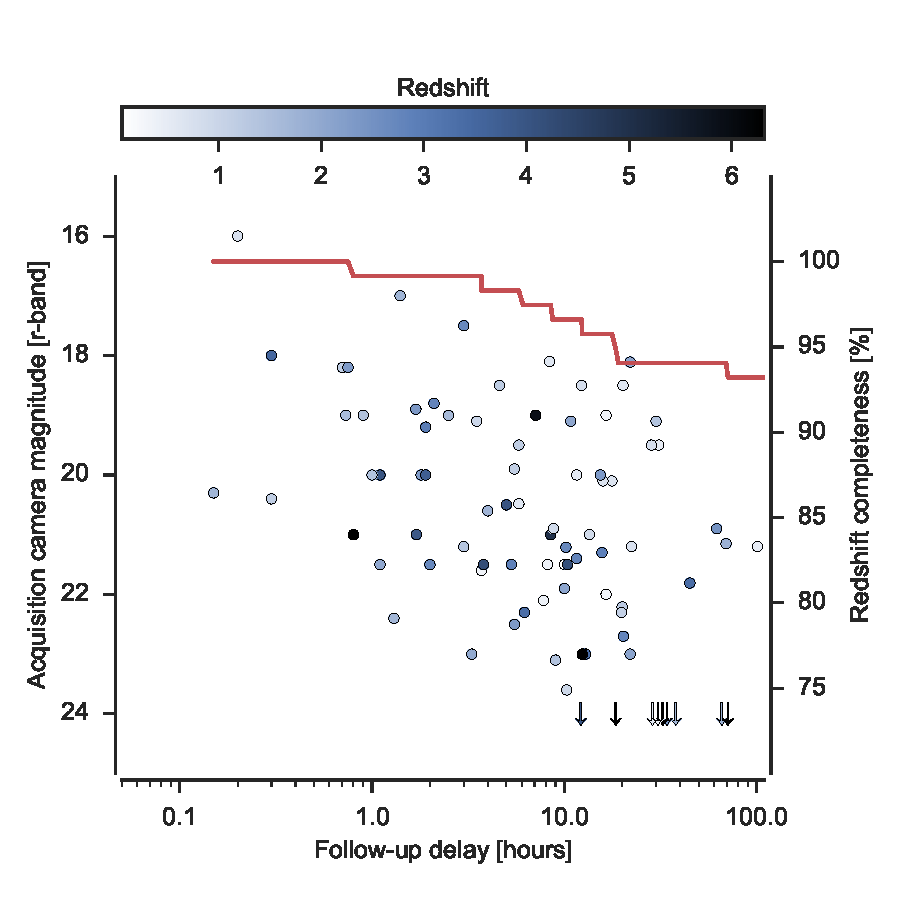
\includegraphics[width=9cm]{figures/timing.pdf}} \caption{Afterglow
	magnitude at the start of observation and redshift completeness as a function
	of follow-up delay for all the afterglows that have been followed up. The
	points have been colored based on the redshift of the corresponding burst. Red
	crosses indicate GRBs without a measured redshift and arrows indicate bursts
	for which the afterglow was not detected in the acquisition image. In red is
	shown the redshift completeness as a function of follow-up delay.}
\label{fig:timing}
\end{figure}
%%%%%%%%%%%%%%%%%%%%%%%%%%%%%%%%%%%%%%%%%%%%%%%%%%%%%%%%%%%%%%%%%%%%%%%%%%%%
\subsection{Sample completeness} \label{completeness}
%%%%%%%%%%%%%%%%%%%%%%%%%%%%%%%%%%%%%%%%%%%%%%%%%%%%%%%%%%%%%%%%%%%%%%%%%%%%

Of all the BAT-triggered bursts, a total of 158 bursts fulfill the sample
criteria specified in Sect. \ref{samplecrit}, since the commissioning of
VLT/X-shooter. This sample constitutes the \textit{statistical sample} from
which we will derive statistical properties of the GRB population. The redshift
completeness of the full statistical sample is 61 per cent. We return to the
question of redshift completeness in Sect. \ref{redshift}. From this sample, 91
GRBs have been spectroscopically followed up with X-shooter. In order to assess
whether the subset of bursts followed up are representative of the underlying
GRB parent population, we compare intrinsic properties of GRBs in our sample to
GRBs in the full sample followed up by \textit{Swift}. We show the comparison
between the BAT (15 -- 150 keV) fluence, the XRT flux (0.3 -- 10 keV) at 11
hours, and the intrinsic X-ray derived equivalent hydrogen column density at the
redshift of the GRB, in excess of the Galactic X-ray absorption column,
$N_{\mathrm{HI,X}}$, in Fig. \ref{fig:swift_complete}. For the latter, we can
only use values of $N_{\mathrm{HI,X}}$ derived for bursts with a measured
redshift, excluding $\sim 75$ per cent of the full \swift~sample. We return to
the last point in Sect. \ref{darkness}.


\begin{figure*}
	\centerline{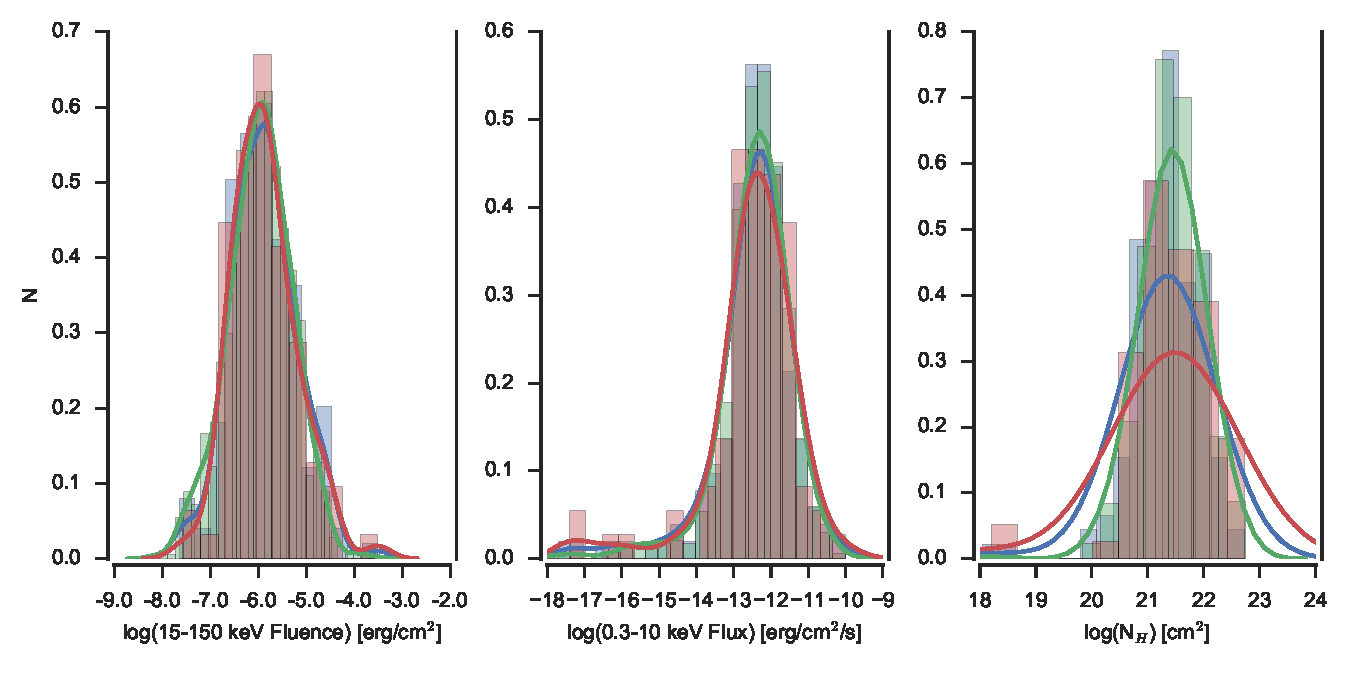
\includegraphics[width=18cm]{figures/completeness_BAT.pdf}}
\caption{Comparison between the burst properties of all bursts observed with
	\textit{Swift} (blue), the statistical sample that fullfill the criteria
	specified in Sect. \ref{samplecrit} (green), and the subset that has been
	observed as part of the statistical sample (red). The left plot shows the
	fluence in 15-150 keV as observed by BAT. The middle panel shows the 0.3 - 10
	keV flux, 11 hours after the bursts as measured by XRT. In the right most
	panel, we show $N_{\mathrm{HI,X}}$ based on the XRT spectrum
	\citep{Evans2009}.} \label{fig:swift_complete}
\end{figure*}

Using the observational characteristics of the 1266 bursts observed until
\termdate~by \textit{Swift}, and the derived $N_{\mathrm{HI,X}}$ \citep{Evans2009}, we can
quantify the degree to which our sample is biased relative to the overall
\textit{Swift} sample. The values are queried from the online \textit{Swift}
database\footnote{\url{http://swift.gsfc.nasa.gov/archive/grb\_table/}}$^,$\footnote{\url{http://www.swift.ac.uk/xrt\_live\_cat/}}. Three samples are of interest in order to assess the completeness of the follow-up campaign (Fig.~\ref{fig:swift_complete}); the full \textit{Swift} sample consisting of all the bursts observed by \textit{Swift} (blue), all the bursts that fulfill the selection criteria imposed in Sect. \ref{samplecrit} (green), and the bursts actually followed up with X-shooter (red).

\begin{table*}[!ht]
	\centering
	\begin{tabular}{cccc}
		\hline
		\hline\noalign{\smallskip}
		{} & {Full \textit{Swift} sample} & {Statistical sample} &  {Followed up bursts} \\
		\hline\noalign{\smallskip}
		N$_{BAT}$ & 981 & 163 & 92\\
		$\log(15-150$keV fluence)  & $-5.9_{-0.6}^{+0.7}$ &  $-5.9_{-0.6}^{+0.7}$ &  $-5.9_{-0.7}^{+0.7}$   \\
		N$_{XRT}$ & 902 & 160 & 90\\
		$\log(0.3-10$keV flux) & $-12.3_{-0.8}^{+0.7}$ &  $-12.4_{-0.8}^{+0.7}$ &  $-12.4_{-0.7}^{+0.9}$  \\
		N$_{\mathrm{HI_x}}$ & 248 & 99 & 79\\
		$\log(\mathrm{N}_{\mathrm{HI_x}})$ & $21.7_{-0.9}^{+0.6}$ &  $21.5_{-3.4}^{+0.7}$ &  $21.6_{-4.5}^{+0.7}$  \\
		\hline\noalign{\smallskip}

\end{tabular} 

\caption{
	Population properties (median and 14th and 86th percentiles as the
	error intervals) for the \textit{Swift sample} and the subset of bursts
	fulfilling the sample criteria. The population characteristics of the three
	samples are very similar, which shows that our selection criteria effectively
	conserve the statistical properties of the underlying population, as least for
	these parameters.  Notice that not all bursts have measurements of the
	quantities we compare. \label{tab:sample_properties}
	}

\end{table*}

For each of the samples, we calculate the median, 14th, and 86th percentiles of
each of the distributions, which can be used as point estimates for the
population distribution. These are provided in Table
\ref{tab:sample_properties}. It can be seen from the values that the three
samples have very similar distributions in terms of the point estimates chosen.
This suggests that our selection criteria are unbiased compared to the
\textit{Swift}-sample and that additionally, the follow-up effort conserves the
distributions of the intrinsic GRB properties (except perhaps for
$N_{\mathrm{HI,X}}$, see Sect. \ref{darkness}).

Additionally, using a 2-sided Kolmogorov-Smirnov test (KS-test), we can assess
the degree to which the null hypothesis, that the two distributions are drawn
from the same parent distribution, can be rejected. We show a graphic
representation of the test statistics in Fig. \ref{fig:p_values}. A high p-value
indicates little evidence against the null hypothesis . The distribution of
$N_{\mathrm{HI,X}}$ exhibits the highest degree of dissimilarity, but the two
distribution are still consistent with being drawn from the same underlying
distribution.

\begin{figure}
	\centerline{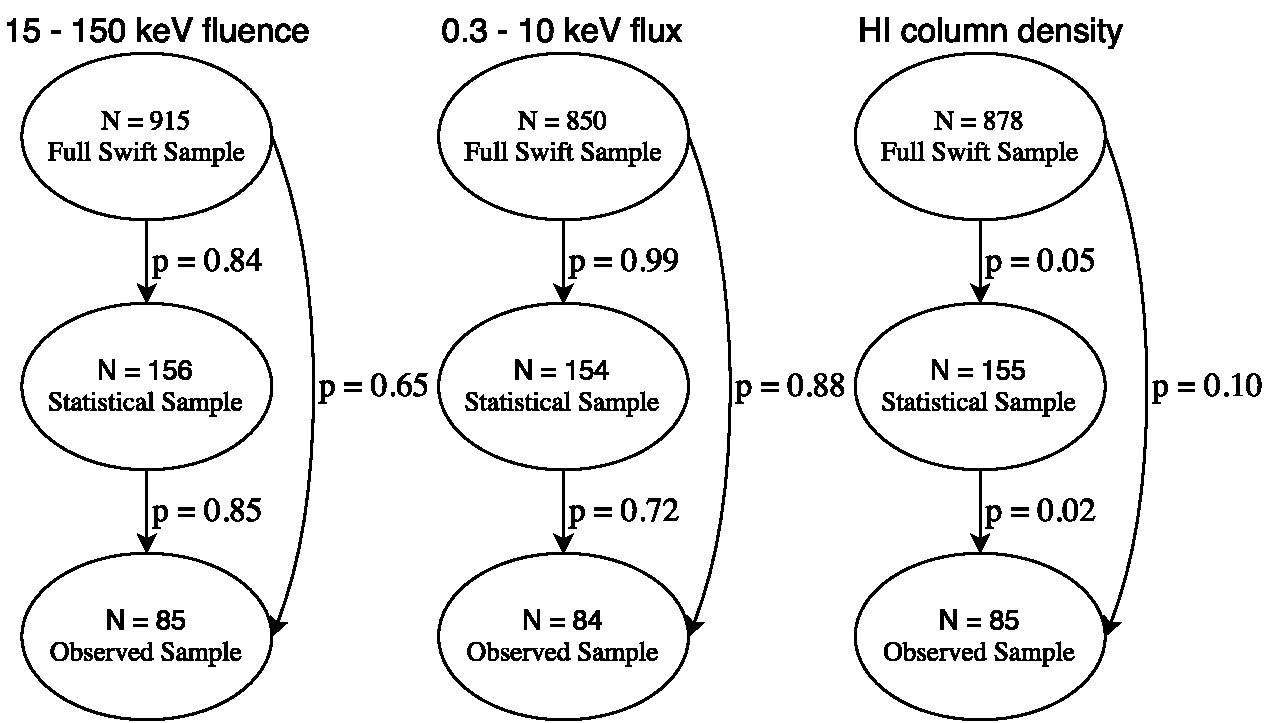
\includegraphics[width=9cm]{figures/XSGRB_p_values.pdf}}
\caption{Relational graph showing the respective p-values. They all represent
	the degree that the different samples are drawn from the same underlying
	distribution. The arrows represent the comparison direction with each of the
	p-values they are listed next to. Only in the H{\sc I} column density distribution is
	there mild evidence against the null hypothesis, but the discrepancy is mainly
	driven by a relatively larger fractional contribution from low-column hosts in
	the statistical sample.} \label{fig:p_values}
\end{figure}

We therefore conclude that the statistics of the sample presented here,
conserves the intrinsic properties of the GRBs in the full \textit{Swift} sample
- at least in terms of BAT fluence and X-ray flux at 11 hours.

%SWIFT LIMITATIONS
%There is some evidence that the burst duration, $T_{90}$, does not scale with
%redshift as expected from time-dilation \citep{Kocevski2013, Littlejohns2013a},
%suggesting that we could be missing an increasing fraction of the bursts at
%higher redshifts, but \citet{Lien2016} argues that we should only be missing the
%bright "short" GRBs", but to the degree that \textit{Swift} is complete, we can
%test if the sample presented here is complete.



%%%%%%%%%%%%%%%%%%%%%%%%%%%%%%%%%%%%%%%%%%%%%%%%%%%%%%%%%%%%%%%%%%%%%%%%%%%%
\subsubsection{Properties of rejected triggers} \label{badbursts}
%%%%%%%%%%%%%%%%%%%%%%%%%%%%%%%%%%%%%%%%%%%%%%%%%%%%%%%%%%%%%%%%%%%%%%%%%%%%

Out of the 158 bursts in the statistical sample, 33 ( $\sim$ 20 per cent) were
not observed due to reasons unrelated to the GRB or afterglow properties. The
reasons include unavailability of the telescope due to technical maintenance
(e.g., mirror re-coating), a visiting observer rejecting the ToO trigger, or bad
weather. Because this cut is unrelated to the GRB properties, it will not change
the statistical properties of the full sample. Removing these bursts for the
statistical sample, dramatically improves the redshift completeness from 61 per cent to 84
per cent. The remaining burst not followed up already had redshift from other
instruments or were very faint and without a host association thus observations
unlikely to yield a redshift measurement. In the remainder of the text, we
consider the 125 bursts our statistical sample.

%%%%%%%%%%%%%%%%%%%%%%%%%%%%%%%%%%%%%%%%%%%%%%%%%%%%%%%%%%%%%%%%%%%%%%%%%%%%
\subsection{On the redshift distribution of GRBs} \label{redshift}
%%%%%%%%%%%%%%%%%%%%%%%%%%%%%%%%%%%%%%%%%%%%%%%%%%%%%%%%%%%%%%%%%%%%%%%%%%%%

One of the objectives of our follow-up campaign is to measure the redshift
distribution for a well-defined, observationally unbiased and statistically useful
sample of GRBs. The imposed selection criteria (see Sect. \ref{samplecrit})
ensure that the GRBs entering our homogeneous sample, fairly represent the
underlying population. The redshift distribution of such a sample holds valuable
information about the occurrence of GRBs through cosmic time
\citep{Jakobsson2012, Perley2016a}.

\begin{table}[H]
	\centering
	\begin{tabular}{ccccc}
		\hline
		\hline\noalign{\smallskip}
		{Sample} & {N$_{\mathrm{bursts}}$} & {$z_{\mathrm{completeness}}$} &  {$z_{\mathrm{mean}}$} &  {$z_{\mathrm{med}}$} \\
		\hline\noalign{\smallskip}
		{\smallskip}
		XS-GRB & 129 & 88 \% & 1.89 & $1.52_{-0.91}^{+1.83}$ \\
		{\smallskip}
		SHOALS  & 119 &  99 \% &  2.18  & $2.06_{-1.20}^{+1.27}$ \\
		{\smallskip}
		BAT6 & 58 & 95 \% &  1.90 &  $1.71_{-1.04}^{+1.31}$ \\
		{\smallskip}
		TOUGH & 69 &  77 \% & 2.20 & $2.11_{-1.36}^{+1.42}$ \\
		{\smallskip}
		Fynbo09 & 146 &  49 \% &  2.2 & $2.1_{-1.23}^{+1.28}$ \\
		\hline\noalign{\smallskip}

\end{tabular} 

\caption{Comparison between the redshift distributions of previous complete
	samples. The SHOALS redshift characteristics are taken from \citet{Perley2016a},
	the BAT6 redshifts are from \citet{Salvaterra2012}, TOUGH is from
	\cite{Hjorth2012}, and Fynbo09 are from \citet{Fynbo2009}. The errors shown on
	the median redshift contain 68 per cent of the probability mass.
	\label{tab:redshift_comparison}}



\end{table}

In Fig.~\ref{fig:z} we show the redshift distribution of all  the observed GRBs.
In the top panel we show a histogram for the full sample and the statistical
sample and in the main panel, we show the redshifts of the individual bursts as
a function of GRB energy in the observed 15 -- 150 keV band. To calculate the
energy, $E_{\mathrm{BAT}}$, we follow a similar procedure as \citet{Lien2016}
and define $E_{\mathrm{BAT}} = F_{\gamma}\,4 \pi\,d_L^2\,(1+z)^{-1}$, where
$F_{\gamma}$ is the observed BAT fluence in the 15-150 keV band and $d_L$ is the
luminosity distance to the burst at the given redshift. Note that this measure
of luminosity does not include any $k$-correction. As an indication of the
effect of the \textit{Swift} sensitivity limit on the redshift distribution,
also in the figure, we have shown the so called $\sim 1$ s flux BAT sensitivity
limit ($\sim 3 \times 10^{-8}~\mathrm{erg}~\mathrm{s}^{-1}~\mathrm{cm}^{-2}$;
\citealt{Baumgartner2013, Lien2016}). Due to the complex triggering mechanism of
\swift, this sensitivity limit should be interpreted with some caution as the
effective limit depends on the light curve of the prompt emission signal. Due to
the dilution of light with distance, the \swift~GRB luminosity detection limit
is almost an order of magnitude brighter at $z=2$ than at $z=1$. At $z\geq4$ we
are only able to observe GRBs that are $\sim$ hundred times brighter than the
faintest bursts at $z=1$ and below. The effect of GRB redshift on the \swift~triggering criteria have previously been studied in detail \citep{Littlejohns2013a}.

We compare the point estimates for the redshift distributions of previous
complete samples of GRBs in Tab. \ref{tab:redshift_comparison}. We see that when
we compare to other complete samples, the XS-GRB presented here has the lowest
average redshift. However, the other samples also exhibit a large spread in the
redshift distributions. A 2-sided KS test confirms that there is only mild
evidence against the Fynbo09 (p-value = 0.05) and TOUGH (p-value = 0.05) samples
being drawn from the same parent sample, while XS-GRB is consistent with the
SHOALS (p-value = 0.08) and BAT6 (p-value = 0.86) samples.

Because the redshift completeness of our statistical sample is 84 per cent,
making inference of the \textit{true} redshift distribution of GRBs based on
this sample is impossible. %The biases introduced in the measured redshift
%distribution by our increased ability to secure redshifts for optically
% brighter
%bursts has been investigated by \citet{Turpin2016} who find that we
%systematically are able to measure redshifts for longer duration GRBs.
%Additionally o
For instance, only the brightest GRBs are seen above redshift $z \gtrsim 1$ as
shown in Fig. \ref{fig:z}. As described in detail in \citet{Hjorth2012} and
\citet{Perley2016b}, bursts for which the redshift is measured from the
afterglow are systematically found for host galaxies with a lower luminosity
than burst for which the redshift is measured from the host galaxy. Only a few
GRBs hosted in galaxies, with stellar masses more than
$10^{10}~\mathrm{M}_\odot$ have the redshift measured based on the afterglow
continuum. This is likely related to the presence of higher contents of dust in
more massive galaxies, leading to a larger fraction of extincted afterglows.



\begin{figure*}
	\centering 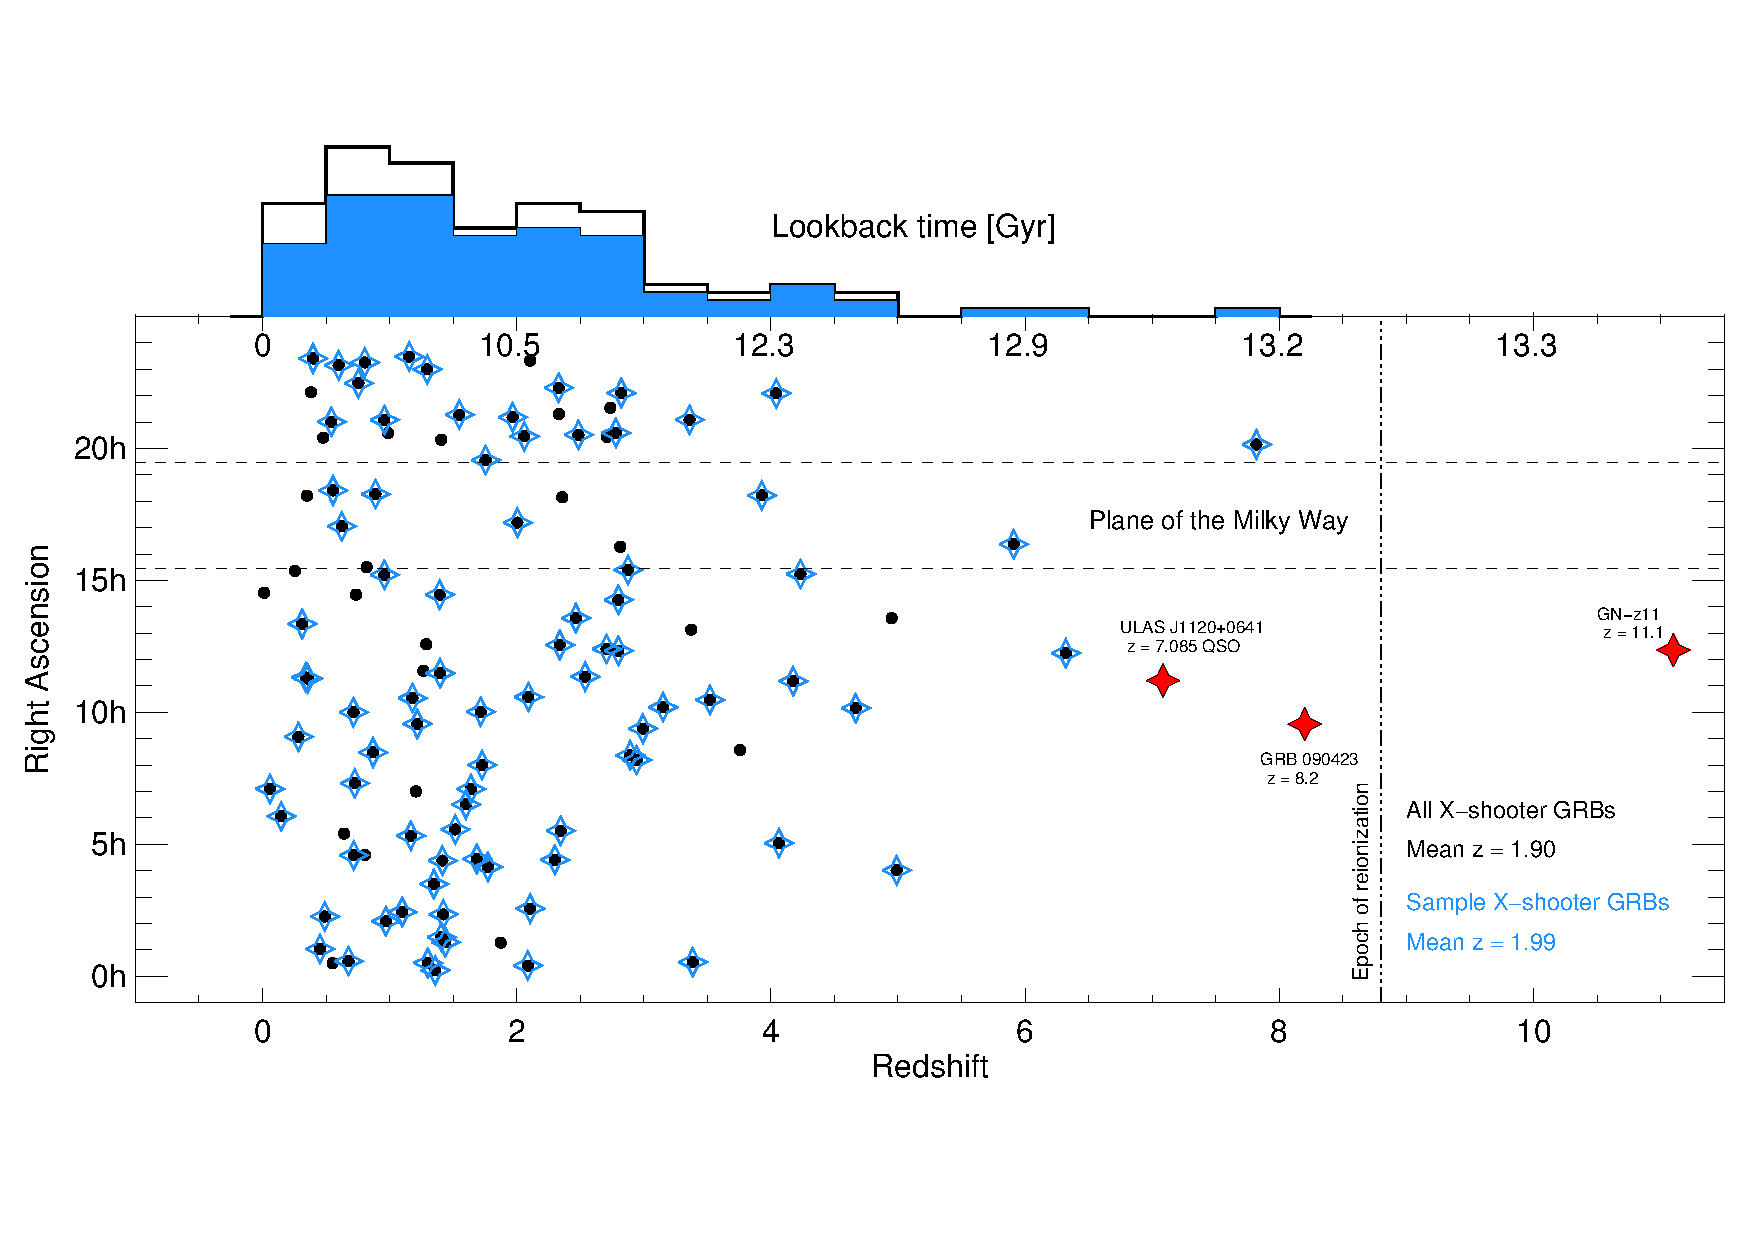
\includegraphics[width=16cm]{figures/XSGRB_redshift.pdf}
\caption{Redshift distribution as a function of intrinsic BAT $\gamma$-ray
	energy, $E_{\mathrm{BAT}}$. Bursts that are a part of the statistical sample
	are marked by blue stars whereas black dots show all GRBs observed with
	X-shooter. All \swift~GRBs with measured redshifts are shown in gray. For
	comparison, we overplot with red stars the GRB \citep{Tanvir2009b,
		Salvaterra2009a}, quasar \citep{Banados2017}, and galaxy \citep{Oesch2016} with
	the highest spectroscopically confirmed redshifts, the latter two shown at
	arbitrary $E_{\mathrm{BAT}}$. The blue solid line represents the so-called 1 s
	BAT sensitivity limit described in the text. The estimated epoch of
	reionization is shown by the black dot-dashed line, with the uncertainty shown
	as the black dashed lines, from the most recent measurement by
	\citet{Planck2015}. On the top of the plot is shown the marginalization of the
	redshift. Again the blue histogram represents the bursts than enter our sample
	and the white histogram the full GRB population. } \label{fig:z}
\end{figure*}



%%%%%%%%%%%%%%%%%%%%%%%%%%%%%%%%%%%%%%%%%%%%%%%%%%%%%%%%%%%%%%%%%%%%%%%%%%%%
\subsection{Sample darkness} \label{darkness}
%%%%%%%%%%%%%%%%%%%%%%%%%%%%%%%%%%%%%%%%%%%%%%%%%%%%%%%%%%%%%%%%%%%%%%%%%%%%

A fraction of all GRBs exhibit no detectable or very faint optical afterglows
\citep{Groot1998, Djorgovski2001, Fynbo2001}. The degree of optical extinction
relative to the X-ray brightness has been parametrized in term of their optical
darkness, using the measurement of, or limit on, the optical to X-ray spectral
index $\beta_{OX}$ \citep{Jakobsson2004, Rol2005, VanderHorst2009}. The X-ray
properties of such bursts have previously been investigated
\citep{DePasquale2003, Fynbo2009, Melandri2012} and there are some indications
that dark bursts have somewhat higher X-ray luminosity and $N_{\mathrm{HI, X}}$
compared to the optically bright bursts \citep{Campana2012}. This indicates along with
investigations of host galaxy properties \citep{Greiner2011, Kruhler2011,
	Hjorth2012, Perley2016b}, that the extinction of the optical afterglows is
primarily driven by the presence of dust in the host galaxies and not solely by
unfortunate placement of the synchrotron spectral break frequencies.
\citet{Hjorth2012} find that systems with no optical afterglow have higher
$N_{\mathrm{HI, X}}$, irrespective of the nature of the host -- which however
also turn out to be redder.

For all bursts with follow-up within 100 hours we calculate the
"darkness"-parameter, $\beta_{OX}$ \citep{Jakobsson2004}. This requires the
simultaneous measurement of the X-ray flux density and the optical flux density
which is in practice is possible, but in reality extremely rarely available. As
a proxy, we use the measured acquisition camera magnitude reported in Table
\ref{tab:sample_overview} to get the optical flux density at the beginning of
the spectroscopic integration. Because we know the delay between the follow-up
and the \textit{Swift} trigger, we can use the measured XRT lightcurve
\citep{Evans2007,
	Evans2009}\footnote{http://www.swift.ac.uk/xrt\_curves/trigger\_numer/flux.qdp}
to infer the corresponding X-ray flux density at the time of the optical
observation. This is done by either linearly interpolating between temporally
neighboring XRT measurements of by extrapolating the last few X-ray data points
to the time of the spectroscopic observation. When the afterglow is not detected
in the acquisition camera, an upper limit of $> 24$ mags is used, which
propagates into an upper limit on $\beta_{OX}$.

In Fig. \ref{fig:betaOX} we compare the $\beta_{OX}$ - $N_{\mathrm{HI, X}}$
distribution with the one presented in \citet{Fynbo2009}. We take the
$N_{\mathrm{HI,X}}$ values from the
\href{http://www.swift.ac.uk/xrt_spectra}{XRT spectral fits} \citep{Evans2009}.
The values from \citet{Fynbo2009} have been treated as detections, meaning that
we artificially bias the distribution towards higher $\beta_{OX}$-values. The
two distributions exhibit a large degree of overlap. We cannot confirm the
result by \citet{Fynbo2009}, that dark bursts, $\beta_{OX} < 0.5$, have higher
\nhx. Specifically, for bursts with measured redshift either from the afterglow
or the host galaxy, we find the following: For bursts with $\beta_{OX} \geq 0.5$
we find \nhx~$ = 21.4_{-1.0}^{+0.7}$, whereas for $\beta_{OX} < 0.5$ we find
\nhx~$21.8_{-0.9}^{+0.5}$ where 68 per cent of the probability mass is contained
within the error intervals. A 2-sided KS test fails to reject the null
hypothesis that they are drawn from the same distribution with $p = 0.43$,
meaning there is no strong evidence for a discrepancy. A Kendall's $\tau$ test
suggest a non-significant, very low degree of negative correlation ($\Gamma =
-0.15$ at a p-value = 0.10).

 
\begin{figure}[!ht]
	\centerline{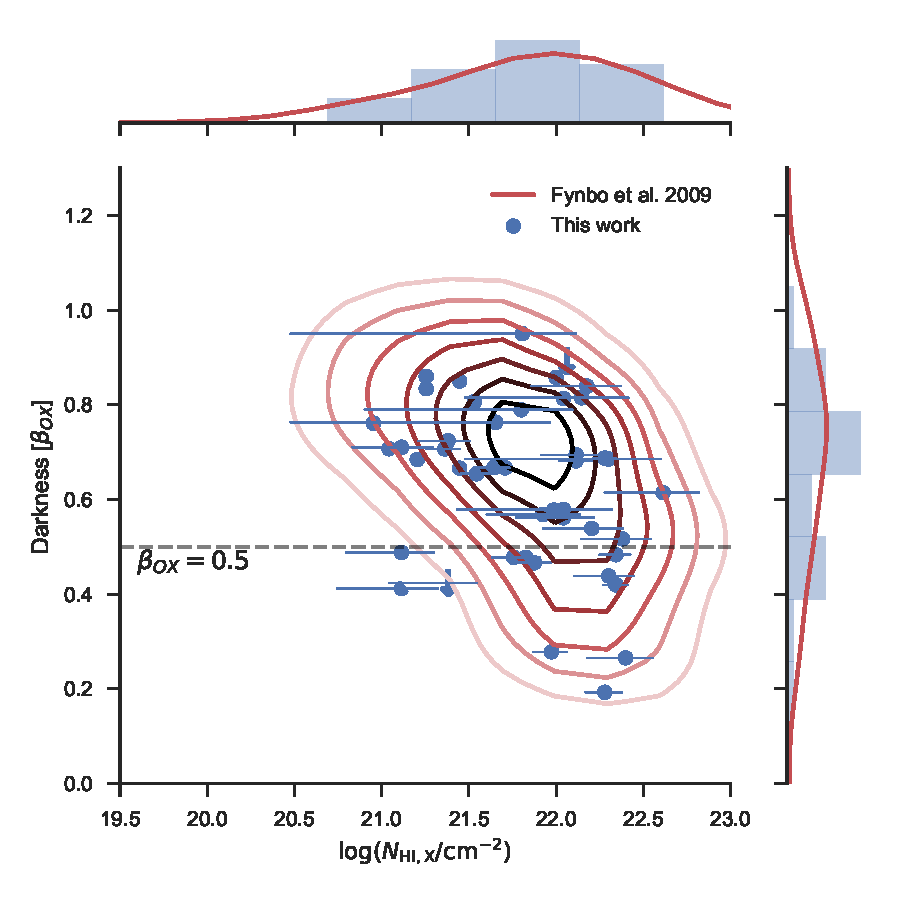
\includegraphics[width=9cm]{figures/betaOX.pdf}} \caption{Optical
	extinction relative to X-ray against X-ray derived hydrogen column densities.
	In red is shown the sample presented in \citet{Fynbo2009} where the lines
	indicate the kernel density estimate of the distribution. For the kernel
	density estimate, the limits have been replaced with values. We note that
	contrary to what is presented in \citet{Fynbo2009}, we exclude all bursts for
	which we do not have a redshift. Darker colors represented higher density of
	points. In blue are the points for the bursts presented here along with the
	marginal histograms. Limits on $\beta_{OX}$ are shown by downwards facing
	arrows. The corresponding marginal distributions are shown along the edges of
	the plot. There is no statistically significant correlation between the two
	quantities.} \label{fig:betaOX}
\end{figure}

Using the table maintained by
J. Greiner\footnote{http://www.mpe.mpg.de/~jcg/grbgen.html}, we can see how the
presence of an optical afterglow affects the follow-up statistics. 50.5 per cent
of all \textit{Swift}-triggered bursts in this list do not have a detected
optical afterglow. This number also includes bursts where no optical
observations were available, so the real number is likely to be lower. For the
bursts that enter our statistical sample, the percentage of bursts without a
detected optical afterglow is 28 per cent, close to the upper limit on the
fraction of dark bursts found in a complete sample with a very high degree of
redshift completeness \citep{Melandri2012}. Of the bursts for which follow-up
has actually been attempted, this number is 23 per cent, suggesting a slight
bias against bursts without a detected optical afterglow in the spectroscopic
sample.

However, the fraction of dark bursts for which we have measured redshifts for is
lower than the for the ones with a detected optical afterglow. For the
afterglows we have observed as part of the statistical sample that do not have a
detected optical afterglow, the redshift completeness is 53 per cent. For
comparison, for the afterglows in the statistical sample we have observed with
an optical afterglow detected, the redshift completeness is 91 per cent. This
also goes to show that the lack of redshift completeness in the sample presented
here is in part due to the increased difficulty of measuring a redshift for
bursts without an afterglow. To measure a redshift, we either need a detected
afterglow to obtain a spectrum or to locate the host galaxy and determine the
redshift from there. It is more difficult to correctly associate a galaxy with a
burst when there is no detected optical afterglow and hence a correct redshift
measurement is more difficult to make, see \citet{Jakobsson2005, Levesque2010}
and \citet{Perley2017}.

Regardless the fraction of dark bursts being lower in the observed sample,
compared to the statistical sample, the X-ray properties do not differ
significantly, as shown in Sect. \ref{completeness}. This is despite
spectroscopic follow-up only being carried out in cases where either a
detectable optical afterglow or a clear counterpart are seen, which naively
should be biased against dark bursts occurring in more obscured galaxies, which
is shown to exhibit different galactic properties \citep{Perley2009,
	Kruhler2011, Rossi2012, Perley2013b, Perley2015b}. That the decreased fraction
of dark bursts in observed sample does not alter the observed prompt X-ray
brightness distribution, potentially reflects the independence of the X-ray
brightness on the density of the circumburst medium \citep{Freedman2001,
	Berger2003, Nysewander2009}, if the measured $N_{\mathrm{HI, X}}$ is primarily
driven by a metal column local to the burst. Because we only use values for
$N_{\mathrm{HI, X}}$ in the comparison for which the GRB has a measured
redshift, this measure is likely biased toward optically brighter bursts.

%%%%%%%%%%%%%%%%%%%%%%%%%%%%%%%%%%%%%%%%%%%%%%%%%%%%%%%%%%%%%%%%%%%%%%%%%%%%
 \subsection{Hydrogen column densities}
%%%%%%%%%%%%%%%%%%%%%%%%%%%%%%%%%%%%%%%%%%%%%%%%%%%%%%%%%%%%%%%%%%%%%%%%%%%%

The locations of long GRBs are associated with intensely star-forming regions
\citep{Hogg1999, Bloom2002, Fruchter2006}. Because a significant fraction of the
hydrogen along the line of sight in these regions has not been ionized, the
optical depth at the wavelength of \lya~is very high, saturating not only the
line center, but also the damping wings. This causes a strong absorption system
from the \lya-transition to appear in the afterglow continuum. For bursts with
$z \gtrsim 1.7$, the position of \lya~moves into the spectroscopic coverage of
X-shooter, meaning that we are able to detect this absorption trough due to
\lya. The exceptionally good UV response of X-shooter, allows us to robustly
measure H{\sc i}-columns - also at these very low redshifts.

Due to the stochastic nature of the \lya-forest, the blue wing of the
Lyman-$\alpha$ absorption line is randomly superposed with Lyman-$\alpha$ forest
systems, along with strong absorption from \mnii~and \SIiii, making it
notoriously difficult to model. Additionally, the red wing has got the ISM
signatures imprinted on it, especially strong absorption due to \SIii, \sii~and
\nv, which can exhibit significant velocity structure. Along with instrumental
effects, the generative model for the data that we would use in a
likelihood-based analysis would be very complicated. We have therefore decided
not to make formal $\chi^2$ fitting of the hydrogen column densities, but
instead use a more subjective visual measurement to the absorption profile. 
Using an analytic approximation to the absorption profile from
\citet{TepperGarcia2006}, we overplot a synthetic absorption line with a
specified column density on our observed, normalised spectrum. By tuning the
value of the hydrogen column density until the synthetic absorption line matches
the spectrum, we can thereby infer the actual column density of the GRB sight
line in a manual way. Similarly, the uncertainty on the hydrogen column can be
estimated by adjusting the error, until the confidence bounds contain the
continuum variation. We show the results of this procedure for all bursts where
possible in Fig. \ref{fig:HI1} and the inferred hydrogen column densities in
Table~\ref{tab:HI}.

\begin{table}[!ht]
\caption{Hydrogen column densities for all bursts exhibiting \lya~absorption in the spectral coverage of X-shooter. Corresponding fits are shown in Fig. \ref{fig:HI1}. \label{tab:HI}}
\centering
\begin{tabular}{cc}
\hline
\hline\noalign{\smallskip}
{GRB} & {Hydrogen Column} \\
\hline\noalign{\smallskip}

GRB~090809A & 21.7 $\pm$ 0.2    \\
GRB~090926A & 21.55 $\pm$ 0.10  \\
GRB~100219A & 21.20 $\pm$ 0.20  \\
GRB~100425A & 21.10 $\pm$ 0.20  \\
GRB~100728B & 21.2 $\pm$ 0.5  \\
GRB~110128A & 22.00 $\pm$ 0.15  \\
GRB~110818A & 21.9 $\pm$ 0.4    \\
GRB~111008A & 22.40 $\pm$ 0.10  \\
GRB~111107A & 21.0 $\pm$ 0.2    \\
GRB~120119A & 22.7 $\pm$ 0.2    \\
GRB~120327A & 22.0 $\pm$ 0.15   \\
GRB~120404A & 20.7 $\pm$ 0.3    \\
GRB~120712A & 19.95 $\pm$ 0.15  \\
GRB~120716A & 22.00 $\pm$ 0.15  \\
GRB~120815A & 22.05 $\pm$ 0.10  \\
GRB~120909A & 21.70 $\pm$ 0.10  \\
GRB~121024A & 21.85 $\pm$ 0.10  \\
GRB~121027A & 22.8 $\pm$ 0.3    \\
GRB~121201A\tablefootmark{a} & 22.0 $\pm$ 0.3  \\
GRB~121229A & 21.7 $\pm$ 0.2    \\
GRB~130408A & 21.8 $\pm$ 0.1    \\
GRB~130427B & 21.9 $\pm$ 0.3    \\
GRB~130606A & 19.91 $\pm$ 0.02  \\
GRB~130612A & 22.1 $\pm$ 0.2    \\
GRB~131011A & 22.0 $\pm$ 0.3    \\
GRB~131117A & 20.0 $\pm$ 0.3    \\
GRB~140311A & 22.40 $\pm$  0.15 \\
GRB~140430A & 21.8 $\pm$ 0.3    \\
GRB~140515A & 19.0 +- 0.5     \\
GRB~140614A & 21.6 $\pm$ 0.3    \\
GRB~141028A & 20.6 $\pm$ 0.15   \\
GRB~141109A & 22.1 $\pm$ 0.1    \\
GRB~150206A & 21.7 $\pm$ 0.4    \\
GRB~150403A & 21.8 $\pm$ 0.2    \\
GRB~150915A\tablefootmark{a} & 21.2 $\pm$ 0.3     \\
GRB~151021A & 22.2 $\pm$ 0.2    \\
GRB~151027B & 20.5 $\pm$ 0.2    \\
GRB~160203A & 21.75 $\pm$ 0.10  \\
GRB~160410A\tablefootmark{b} & 21.2 $\pm$ 0.2 \\
GRB~161014A & 21.4 $\pm$ 0.3    \\
GRB~161023A & 20.96 $\pm$ 0.05  \\



\hline\noalign{\smallskip}

\end{tabular}
\tablefoot{
\tablefoottext{a}{Has \lya~emission in the trough.}
\tablefoottext{b}{Short burst.}
} 
\end{table}

In the compilation of $N_{\mathrm{HI}}$ measurements towards GRBs in Tanvir et
al. (submitted) %\citet{Tanvir2017}
there are 81 published $N_{\mathrm{HI}}$ values, excluding the measurements
provided here. We here provide 39 new neutral hydrogen column density
measurements -- an increase of the number of optically derived hydrogen column
densities of $\sim$ 50 per cent. We show the two distributions in  Fig.
\ref{fig:NH_dist}. We compare the median, the 14th, and 86th percentiles of the
two distributions. The sample presented has a \nh~$= 21.8_{-0.8}^{+0.3}$ and the
rest of the literature values has \nh~$= 21.5_{-1.5}^{+0.4}$. We see that the
two distributions have a large degree of overlap due to the large width of the
distributions, but we find a slightly higher median value for the new sample
presented here. A 2-sided KS test gives a p-value of p = 0.006, meaning
relatively large evidence against the null that the two samples are drawn from
the same underlying distribution. Because the bursts that have measurements of
the hydrogen column density are selected solely based on our ability to infer a
column, it is difficult to make any strong conclusions about the population
statistics in terms of gas content.

In Fig. \ref{fig:NH_dist}, we also show the column density-distribution
for the 12081 quasar absorbers with \nh~$> 20$ from \citet{Noterdaeme2012b}. The
fact that GRBs systematically are located behind the highest \nh, previously
noted \citep[e.g.,][]{Prochaska2007, Fynbo2009}, is very clear in this
figure. The reason for this is that quasar sample sight-lines through galaxies
that are cross-section selected, whereas GRB sight-lines probe the dense,
star-forming regions in their hosts.

\begin{figure}[!ht]
	\centering 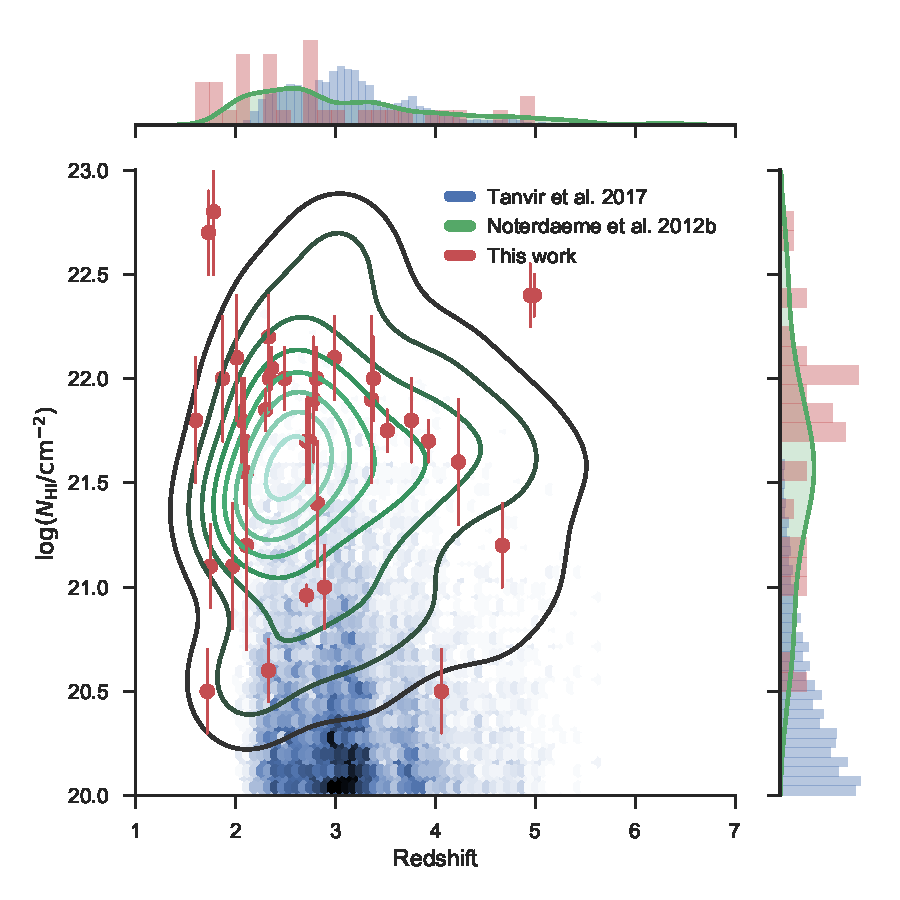
\includegraphics[width=9cm]{figures/NH_dist.pdf}
\caption{Distributions of hydrogen column densities for absorbers found in
	quasar absorption lines, from \citet{Noterdaeme2012b} in blue. Overplotted in
	green is the kernel density estimate of absorbers in GRB sightlines. Values are
	taken from the compilation in Tanvir et al. (submitted), along with the new
	values presented in this sample. We also show in the red the values derived in
	this work. The marginal distributions for the three distributions are also shown
	along the left side and on the top, where the different environments probed are
	clearly visible in the hydrogen column densities, as previously also noted in
	\citet{Fynbo2009}.} \label{fig:NH_dist}
\end{figure}



%%%%%%%%%%%%%%%%%%%%%%%%%%%%%%%%%%%%%%%%%%%%%%%%%%%%%%%%%%%%%%%%%%%%%%%%%%%%
\section{Discussion and conclusions}\label{conclusions}
%%%%%%%%%%%%%%%%%%%%%%%%%%%%%%%%%%%%%%%%%%%%%%%%%%%%%%%%%%%%%%%%%%%%%%%%%%%%

In this paper we have presented the results of a dedicated effort over the years
2009 -- 2017 to use the X-shooter spectrograph on the ESO-VLT to secure
spectroscopic observations of afterglows and host galaxies of GRBs detected by
\swift. This work was initiated by a consortium using Guaranteed Time on
X-shooter, but over the years the project continued in open time.

The sample presented here includes spectroscopic observations of 91 systems
fulfilling our sample criteria, including 18 spectra that are late-time
observations of the underlying host galaxies. All spectra have been made
publicly available in the reduced form used in this paper.

Our sample serves the purpose to further characterize the environments of GRBs
that was also much advanced by the previous surveys based primarily on
lower-resolution spectrographs. GRB afterglow sight-lines are unique in the
sense that only after observing more than 12000 damped Lyman-$\alpha$ absorbers
(DLAs) towards about 10$^5$ quasars, a handful systems with \nh~$ > 22$ been
identified \citep[e.g., five in][]{Noterdaeme2012b}. Long GRB afterglow spectra,
by contrast, reveal such systems in the majority of cases \citep[][and this
work]{Jakobsson2006b, Fynbo2009, Cucchiara2015}. With afterglow spectroscopy
(throughout the electromagnetic spectrum from X-rays to the sub-mm) we are able
to characterize the properties of star-forming galaxies over cosmic history in
terms of redshifts, metallicities, molecular contents, ISM temperatures, UV-flux
densities, extinction curves, etc.  A number of independent papers have been
published or submitted for publication focusing on many of these specific issues
of our sample such as extinction curves \citep[][see also \citealt{Fynbo2014,
	Heintz2017}]{Japelj2015, Zafar17}, emission lines from the underlying host
galaxies \citep{Kruhler2015}, the frequency of intervening \mgii~ absorbers
\citep{Christensen2017}, \citet{Arabsalmani2018} on the metallicity-scaling
relations, and escape of ionizing radiation (Tanvir et al., submitted). A number
of additional companion papers are also planned, investigating the detailed
properties of the sample presented here, including equivalent width
distributions (de Ugarte Postigo et al., in preparation), metallicities and
kinematics (Th{\"o}ne et al., in preparation), high ionization lines (Heintz et
al., in preparation), molecular lines (Bolmer et al., in preparation),
fine-structure lines (Vreeswijk et al., in preparation), composite GRB afterglow
spectrum (Selsing et al., in preparation).

The potential of using GRB sightlines as probes is far from fully harvested. The
sample of sightlines probed by our spectra are not representative for all GRB
sightlines as we have shown and consistent with earlier findings from samples
based on low-resolution spectroscopy \citep[e.g.,][]{Fynbo2009} and from studies
of complete samples of GRB host galaxies \citep{Hjorth2012, Covino2013,
	Perley2016}. \cite{Kruhler2013} argue, that very rich sightlines like that
probed by the remarkable GRB~080607 \citep{Prochaska2009} are probably
significantly more frequent than in the sightlines sampled by our spectra.
However, with current instrumentation, these sightlines are out of reach except
under very fortunate circumstances as in the case of GRB~080607 when the
afterglow could be observed only a few minutes after the burst with a 10-m class
telescope. Observations of such sightlines with X-shooter-like spectrographs on
the next generation of 20--40-m telescopes is likely to be very rewarding, given
that a suitable GRB detector will be available.

\begin{acknowledgements}
	*** We should add an acknowledgment to Neil Gehrels and Javier Gorosabel here
***. 
%
JPUF, BMJ and DX acknowledge support from the ERC-StG grant EGGS-278202.
The Dark Cosmology Centre were funded by the Danish National Research
Foundation. 
%
This work was supported by a VILLUM FONDEN Investigator grant to JH
(project number 16599). 
%
TK acknowledges support by the European Commission
under the Marie Curie Intra-European Fellowship Programme in FP7.  
%
JJ acknowledges
support from NOVA and NWO-FAPESP grant for advanced instrumentation in
astronomy. 
%
KEH and PJ acknowledge support by a Project Grant (162948--051) from
The Icelandic Research Fund. 
%
AG acknowledges the financial support from the
Slovenian Research Agency (research core funding No. P1-0031 and project grant
No. J1-8136). 
%
CT acknowledges support from a Spanish National Research Grant of Excellence
under project AYA 2014-58381-P and funding associated to a Ramón y Cajál
fellowship under grant number RyC-2012-09984.
%
AdUP acknowledges support from a Ramón y Cajal fellowship, a BBVA Foundation
Grant for Researchers and Cultural Creators, and the Spanish Ministry of Economy
and Competitiveness through project AYA2014-58381-P.
%
ZC acknowledges support from the Spanish research project AYA 2014-58381-P and
support from Juan de la Cierva Incorporaci\'on fellowships IJCI-2014-21669.
%
AK acknowledges support from the Spanish research project AYA 2014-58381-P and
support from Juan de la Cierva Incorporaci\'on fellowships IJCI-2015- 26153.
%
RSR acknowledges AdUP's BBVA Foundation Grant for Researchers and Cultural
Creators and support from ASI (Italian Space Agency) through the Contract n. 2015-046-R.0 and from European Union Horizon 2020 Programme under the AHEAD project (grant agreement n. 654215).
%
This work made use of data supplied by the UK {\it Swift} Science Data Centre at
the University of Leicester. Finally, it is with pleasure that we acknowledge
expert support from the ESO staff at the Paranal and La Silla observatories in
obtaining these target of opportunity data.


\end{acknowledgements}


\bibliographystyle{mnras}
\bibliography{XSGRB_sample}


\clearpage

\begin{figure*}[!h]
	\centering
	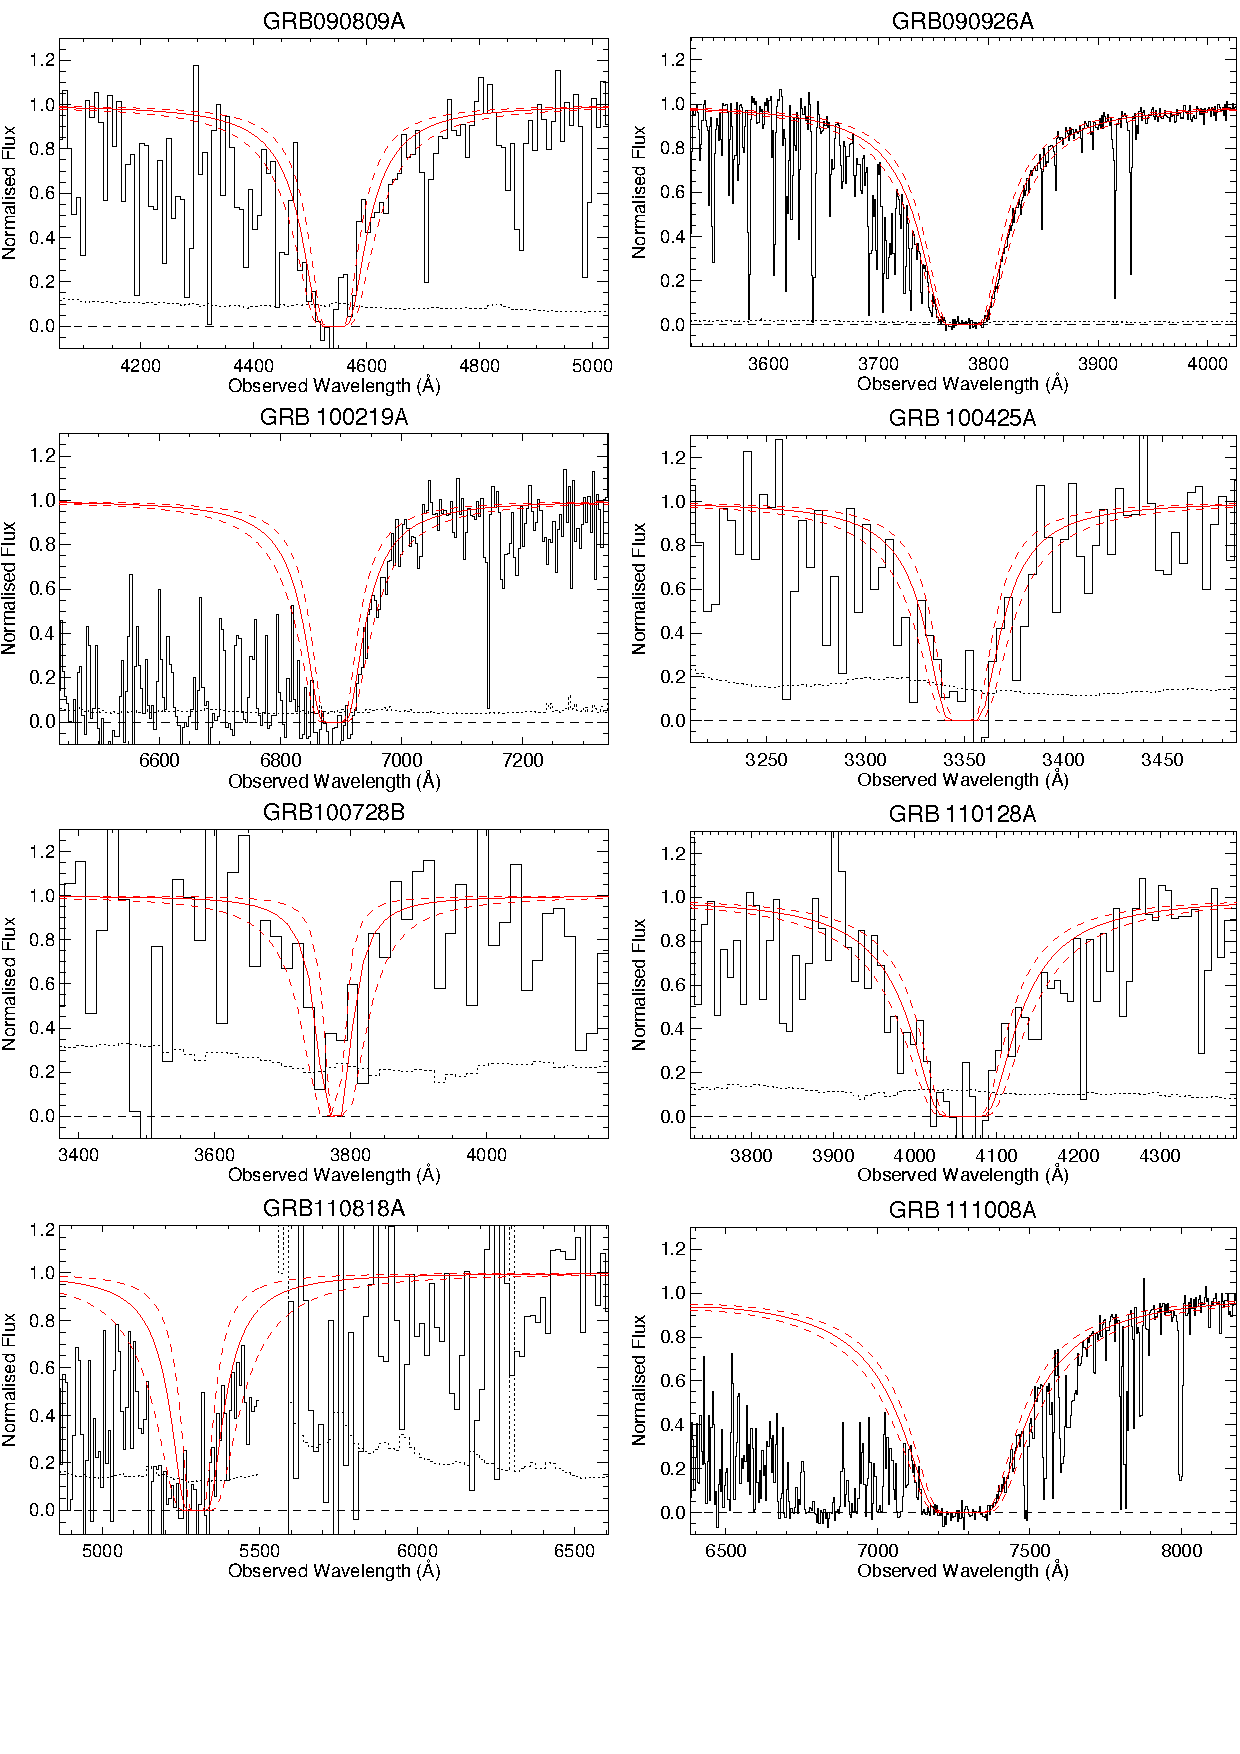
\includegraphics[page=1, width=16cm]{figures/HI_measurements.pdf}
	\caption{Measurements of the hydrogen column-densities for all bursts with a
		clear Lyman alpha absorption system. In solid black is shown the spectrum with
		black dotted giving the corresponding 1-$\sigma$ error. Black dashed shows zero
		flux density. The solid red line is the absorption of column density equal to
		the value presented in Tab. \ref{tab:HI} with the 1-$\sigma$ interval shown
		with dashed lines.}
	\label{fig:HI1}
\end{figure*}
\clearpage
\begin{figure*}[!h]
	\centering
	\includegraphics[page=2, width=16cm]{figures/HI_measurements.pdf}
	\caption*{Fig. \ref{fig:HI1}. continued.}
	\label{fig:HI2}
\end{figure*}
\clearpage
\begin{figure*}[!h]
	\centering
	\includegraphics[page=3, width=16cm]{figures/HI_measurements.pdf}
	\caption*{Fig. \ref{fig:HI1}. continued.}
	\label{fig:HI3}
\end{figure*}
\clearpage
\begin{figure*}[!h]
	\centering
	\includegraphics[page=4, width=16cm]{figures/HI_measurements.pdf}
	\caption*{Fig. \ref{fig:HI1}. continued.}
	\label{fig:HI4}
\end{figure*}
\clearpage
\begin{figure*}[!h]
	\centering
	\includegraphics[page=5, width=16cm]{figures/HI_measurements.pdf}
	\caption*{Fig. \ref{fig:HI1}. continued.}
	\label{fig:HI5}
\end{figure*}
\clearpage




\appendix


%%%%%%%%%%%%%%%%%%%%%%%%%%%%%%%%%%%%%%%%%%%%%%%%%%

\section{The complex error function and the Voigt profile} \label{voigt}
When modeling the spectral PSF, we need to evaluate the Voigt-profile. The Voigt profile, which is the convolution of the Gaussian and Lorentzian profiles, can, centered at zero, be written as \citep{pagnini2010} 
\begin{equation} 
\begin{split}
V(\lambda,\sigma, \gamma)  
& = G(\lambda, \sigma)  \otimes L(\lambda, \gamma) \\
& = \int_{-\infty}^{\infty} G(\xi, \sigma) L(\lambda - \xi, \gamma) d\xi \\
& = \int_{-\infty}^{\infty} \frac{1}{\sqrt{2 \pi} \sigma} e^{- \left( \frac{\xi}{\sqrt{2} \sigma}  \right)^2 } \frac{1}{\gamma \pi} \frac{\gamma^2}{(\lambda - \xi)^2 + \gamma^2} d\xi \\
& = \frac{\gamma}{\sqrt{2} \sigma} \frac{1}{ \pi^{3/2}}   \int_{-\infty}^{\infty} \frac{e^{- \left( \frac{\xi}{\sqrt{2} \sigma}  \right)^2 }}{(\lambda - \xi)^2 + \gamma^2}.
\end{split}
\end{equation}
We can by making the following substitution, $\xi = \sqrt{2} \sigma$ and $d\xi = \sqrt{2} \sigma dt$, write it as
\begin{equation} 
\begin{split}
V(\lambda,\sigma, \gamma)  
& =  \frac{\sqrt{2} \sigma}{ \sqrt{{\pi}}} \frac{\frac{\gamma}{\sqrt{2} \sigma}}{\pi}  \int_{-\infty}^{\infty} \frac{e^{- t^2 }}{(\lambda - \sqrt{2} \sigma t)^2 + \gamma^2} dt \\
& = \frac{1}{\sqrt{2 \pi} \sigma}  \frac{\frac{\gamma}{\sqrt{2} \sigma}}{\pi}  \int_{-\infty}^{\infty} \frac{e^{- t^2 }}{\left(\frac{\lambda}{\sqrt{2} \sigma} -  t\right)^2 + \left(\frac{\gamma}{\sqrt{2} \sigma}\right)^2} dt.	
\end{split}
\end{equation}
This form of the convolution is closely related to the complex probability function \citep{letchworth2007, abrarov2015a},
\begin{equation} 
\begin{split}
W(z)  
& = \frac{i}{\pi} \int_{-\infty}^{\infty} \frac{e^{-t^2}}{z - t}  
\end{split}
\end{equation}
for any complex argument, $z = x + iy$. The complex probability function can be expressed as a sum of a real and an imaginary part \citep{benner1995, abrarov2015b},
\begin{equation} 
\begin{split}
W(x, y)  
& = K(x, y) + i L(x, y) \\
& = \frac{y}{\pi}  \int_{-\infty}^{\infty} \frac{e^{- t^2 }}{(x -  t)^2 +y^2} dt  + \frac{i}{\pi}  \int_{-\infty}^{\infty} \frac{(x - t)e^{- t^2 }}{(x -  t)^2 +y^2} dt,
\end{split}
\end{equation}
where the real part, $\mathtt{Re}[W(x, y)] =  \sqrt{2 \pi} \sigma
V(\lambda,\sigma, \gamma)$ if $x = \frac{\lambda}{\sqrt{2} \sigma}$ and $y =
\frac{\gamma}{\sqrt{2} \sigma}$, which can be obtained by using the complex
argument, $z = \frac{\lambda + i\gamma}{\sqrt{2} \sigma}$, in the complex
probability function. If $\mathtt{Im}[z] \geq 0$, which is always guaranteed for
the width of a spectral profile, the complex probability function equals the
complex error function. The complex error function has numerous, fast, numerical
approximations where in this work we use the \texttt{scipy.special.wofz}
\citep{scipy} implementation.

%%%%%%%%%%%%%%%%%%%%%%%%%%%%%%%%%%%%%%%%%%%%%%%%%%

\section{Notes on Individual objects} \label{notes}

\subsection{GRB~090313 (z = 3.373)} \label{090313}

The first GRB ever observed with X-shooter, during the commissioning of the
instrument, this data formed the basis of GCN
\#9015\footnote{\url{http://gcn.gsfc.nasa.gov/gcn3/9015.gcn3}} and is published
in \citet{DeUgartePostigo2010}. Due to the lingering brightness of GRB~090313,
6.9 ks spectroscopic integration starting 45 hours after the BAT trigger reveals
a wealth of absorption features superposed on the afterglow continuum at a
common redshift of $z = 3.373$. Two intervening systems at $z = 1.959$ and $z =
1.800$ are identified based on strong \mgii-absorption. Because this burst is
observed before the instrument is science-verified, it does not enter into the
statistical sample.

\subsection{GRB~090530 (z = 1.266)}\label{090530}

Observed during paranalization of the instrument, this data forms the basis of
GCN \#15571\footnote{\url{http://gcn.gsfc.nasa.gov/gcn3/15571.gcn3}}, but is not
published elsewhere. Observations began 20.6 hours after the BAT trigger and 4.8
ks spectroscopic integration in all three arms reveals the absorption signature
for a host at $z = 1.266$ from the detection of \mgii, \mgi, \SIii, \feii,
\aliii. Because this burst was observed before the instrument is
science-verified, it does not enter into the statistical sample.

\subsection{GRB~090809 (z = 2.737)} \label{090809}

Observed during the first science verification period and was reported in GCN
\#9761\footnote{\url{http://gcn.gsfc.nasa.gov/gcn3/9761.gcn3}} and is
additionally used as the basis for the master thesis by \'Asa Sk\'ulad\'ottir
(2010). 7.2 ks integration starting 10.2 hours after the GRB trigger yields a
clear afterglow continuum in all arms. The simultaneous detection of absorption
lines identified as \lya, \SIii, \oi, \SIi$^*$, \SIiv, \civ, \feii, \alii,
\aliii~and \mgii~at $z = 2.737$ sets it as the redshift of the GRB. Because this
burst is observed before the instrument was science-verified, it does not enter
into the statistical sample.

\subsection{GRB~090926 (z = 2.106)} \label{090926}

Obtained during the second science
verification period, this dataset forms the basis of GCN
\#9942\footnote{\url{http://gcn.gsfc.nasa.gov/gcn3/9942.gcn3}} and is
additionally published in \citet{DElia2010}. Spectroscopic integration started
22 hours after the BAT trigger and from the acquisition camera the optical
afterglow is measured to R = 17.9 mag at the beginning of the observations which
causes a strong continuum to be seen in all arms. An absorption trough due to
\lya is clearly visible along with numerous metal resonance lines \civ, \SIii,
\SIii$^*$ \feii, \mgii, all at $z = 2.106$. Because this burst was observed
before the instrument is science-verified, it does not enter into the
statistical sample.

\subsection{GRB~091018 (z = 0.971)}\label{091018}

The first burst observed during normal operation after science verification was
completed and there is the first burst that enter the statistical sample. This
data is the basis for GCN \#
10042\footnote{\url{http://gcn.gsfc.nasa.gov/gcn3/10042.gcn3}} and is published
in \citet{Wiersema2012}. With a bright afterglow and a rapid follow-up, this
spectrum is of pristine quality. The afterglow continuum is bright throughout
all spectroscopic arms which allows the ready detection of \alii, \aliii, \feii,
\mnii, \mgii, \mgi, and \caii~- al located at $z = 0.971$, setting is as the
redshift of the host.

\subsection{GRB~091127 (z = 0.490)} \label{091127}

Obtained 4 days after the burst trigger, this data forms the basis for GCN \#
10233\footnote{\url{http://gcn.gsfc.nasa.gov/gcn3/10233.gcn3}} and is published
in \citet{Vergani2011}. Due to the late follow-up and a nearby moon, the signal-to-noise of
the afterglow continuum is low especially in the UVB arm, why no clear
absorption lines are detected against the afterglow continuum, although see
\citet{Vergani2011} which report a tentative detection of \mgii. Emission lines
from the underlying host is clearly visible with lines from \oii, \hb, \oiii,
and \ha~all at $z = 0.490$. This bursts is additionally associated with
SN2009nz.

\subsection{GRB~100205A  (z = na)} \label{100205}

Observed 3 days after the \textit{Swift} trigger. No afterglow or host detected
in 10.8 ks. GRB likely located at high
redshift\footnote{\url{http://gcn.gsfc.nasa.gov/gcn3/10399.gcn3}}. The spectrum
has not otherwise been published previously.

\subsection{GRB~100219A (z = 4.667)} \label{100219}

The data presented here also formed the basis of GCN \#
10441\footnote{\url{http://gcn.gsfc.nasa.gov/gcn3/10441.gcn3}} and is published
in \citet{Thone2013}. Observations started 12.5 hours after the \textit{Swift}
trigger and has a total exposure time of 4.8 ks. Absorption features, including
those of \lya~and from a multitude of ions are detected against the afterglow
continuum at $z = 4.667$. Additionally, absorption from an intervening system
is found at $z = 2.181$.

\subsection{GRB~100316B (z = 1.180)} \label{100316}

The data presented here also formed the basis of GCN \#
10495\footnote{\url{http://gcn.gsfc.nasa.gov/gcn3/10495.gcn3}}. The spectrum
has not otherwise been published previously. Observations started 44 minutes
after the \textit{Swift} trigger and has a total exposure time of 2.4 ks.
Absorption features from \feii, \alii, \aliii,	\mgii~and \mgi~are well detected
against the afterglow continuum at $z = 1.180$. Additionally, strong absorption
lines from \feii~and \mgii~from an intervening system are found at $z = 1.063$.

\subsection{GRB~100316D (z = 0.059)} \label{100316}

The data presented here also formed the basis of GCN \#
10512\footnote{\url{http://gcn.gsfc.nasa.gov/gcn3/10512.gcn3}}, GCN \#
10513\footnote{\url{http://gcn.gsfc.nasa.gov/gcn3/10513.gcn3}}, GCN \#
10543\footnote{\url{http://gcn.gsfc.nasa.gov/gcn3/10543.gcn3}} and is published
in \citet{Bufano2012} and \citet{Starling2011}. This GRB is very close by and
has an associated SN, SN2010bh, and has therefore undergone intense follow-up. The data
presented here consists of a subset of the entire VLT/X-shooter campaign,
covering the four first observing days while the afterglow still contributes
significantly to the total emission. The first observations started 10 hours
after the burst, before the SN was discovered, and targeted the star-forming
'A'-region\citep{Starling2011}, not the GRB. A very rich spectrum containing a
multitude of emission lines puts the host at $z = 0.059$. For three consequtive
nights, 58, 79 and 101 hours after the \textit{Swift} trigger, the afterglow
was observed as it transitioned into the spectrum of a high-velocity Ic-BL SN.
The observations taken 79 and 101 hours after the burst are taken under
programme 084.D-0265(A) (PI: Benetti), but with an identical setup to the first
two observations.

\subsection{GRB~100418A (z=0.624)} \label{100418}

The data presented here also formed the basis of GCN \#
10620\footnote{\url{http://gcn.gsfc.nasa.gov/gcn3/10620.gcn3}} and GCN \#
10631\footnote{\url{http://gcn.gsfc.nasa.gov/gcn3/10631.gcn3}} and is published
in \citet{DeUgartePostigo2011}. The burst have been followed up in three epochs
of observations, 0.4, 1.4, and 2.4 days after the burst, each lasting 4.8 ks.
The unambiguous redshift of the host, $z=0.624$, is found from the simultaneous
detection of emission features belonging to nebular lines, including \hi, \oii,
\oiii, \neiii, \nii, \sii, \siii, and \hei~as well as absorption features due to
the presence of \znii, \crii, \feii, \mnii, \mgii, \mgi, \tiii, and \caii, all
at a consistent redshift. Temporal evolution of the fine structure lines
belonging to \feii$^*$ is found between the epochs.

\subsection{GRB~100424A (z=2.465)} \label{100424}

The data presented here also formed the basis of GCN \#
14291\footnote{\url{http://gcn.gsfc.nasa.gov/gcn3/14291.gcn3}}. The spectrum has
not otherwise been published previously. Observations carried out, long after
the burst has faded.  Emission lines from the host are detected at $z=2.465$.

\subsection{GRB~100425A (z=1.1755)} \label{100425}

The data presented here also formed the basis of GCN \#
10684\footnote{\url{http://gcn.gsfc.nasa.gov/gcn3/10684.gcn3}} and is used in
Skuladottir (2010), but not published elsewhere. Observations started 4 hours
after the \textit{Swift} trigger, totaling 2.4 ks. Absorption features from
\mgii~and \feii~in the afterglow continuum are detected at $z=1.1755$.

\subsection{GRB~100615A (z=1.398)} \label{100615}

The data presented here also formed the basis of GCN \#
14264\footnote{\url{http://gcn.gsfc.nasa.gov/gcn3/14264.gcn3}}, but not
published elsewhere. Host observation of a dark burst\citep{DElia2011} taken
long after the afterglow has faded. Emission lines from the host belonging to
\oii, \neiii, \oiii~and \ha~are detected at a common redshift of $z=1.398$.

\subsection{GRB~100621A (z=0.542)} \label{100621}

The data presented here also formed the basis of GCN \#
10876\footnote{\url{http://gcn.gsfc.nasa.gov/gcn3/10876.gcn3}}, but not
published elsewhere. Beginning 7.1 hours after the GRB, 2.4 ks observations
reveal emission lines from \oii, \hb~and \oiii~at a common redshift of $z=0.542$
and a very weak afterglow continuum.

\subsection{GRB~100625A (z=0.452)} \label{100625}

The data presented here is of the candidate host galaxy, taken long after the
burst has faded and have not previously been published. 4.8 ks of exposure
reveals a weak continuum present in all arms, but an absence of emission lines.
This could indicate that the host primarily contains a older stellar
population. The redshift, $z=0.452$, is taken from \citet{Fong2013}.


\subsection{GRB~100724A (z = 1.288} \label{100724}

The data presented here also formed the basis of GCN \#
10971\footnote{\url{http://gcn.gsfc.nasa.gov/gcn3/10971.gcn3}}. The spectrum has
not otherwise been published previously. The observations were carried out in
RRM starting 11 min after the GRB trigger. See section \ref{RRM}, for a
description of the RRM scheme. Absorption lines from several ionic species are
detected in the afterglow continuum at a common redshift of $z = 1.288$. This is
not a part of the statistical sample.

\subsection{GRB~100728B (z=2.106)} \label{100728}

The data presented here also formed the basis of GCN \#
11317\footnote{\url{http://gcn.gsfc.nasa.gov/gcn3/11317.gcn3}}. The spectrum has
not otherwise been published previously. Starting 22 hours after the burst
trigger, 7.2 ks of observations reveals a faint afterglow continuum with \lya-
and \mgii-absorption at $z=2.106$. Due to a malfunctioning ADC, the sensitivity
of X-shooter is depressed with respect to normal operations, resulting in a
lower throughout. Additionally, the position of the trace on the slit moves due
to atmospheric differential refraction. The presence of the DLA is confirmed in
the 2D image and despite the observational challenges that affects this burst,
we measure \nh~$=21.2 \pm 0.15$.

\subsection{GRB~100814A (z=1.439)} \label{100814}

The spectra presented here has not been published previously. The observations
consists of three visits, the first beginning only 0.9 hours after the
\textit{Swift} trigger, the other two visits were 2.13 and 98.40 hours after the
trigger, respectively. A bright afterglow continuum is present in all visits,
allowing identification of absorption features belonging to a wide range of ions
at $z=1.439$. A complex velocity structure in the absorption features belonging
to \mgii, shows several components, separated by as much as 500km/s, pointing to
a likely merger scenario in the host.

\subsection{GRB~100816A (z=0.805)} \label{100816}

The data presented here also formed the basis of GCN \#
11123\footnote{\url{http://gcn.gsfc.nasa.gov/gcn3/11123.gcn3}}. The spectrum has
not otherwise been published previously. This short GRB was observed 28.4 hours
after the GRB trigger. 4 x 1200 s of exposure reveals two distinct sets of
emission lines, spatially offset $\lesssim 1 \arcsec $, very close in redshift
space, $z=0.8034$ and $z=0.8049$, indicating either an interacting host or some
complex velocity structure of the host. Faint underlying continua are present
under both sets of lines.

\subsection{GRB~100901A (z=1.408)} \label{100901}

The data presented here has been published in \citet{Hartoog2013}. Because of
the unusual lingering brightness of this GRB, 2.4s of observations taken 65.98
hours after the GRB trigger still reveals an afterglow continuum visible across
the entire spectral coverage of X-shooter. Absorption lines from a wide range
ion put the redshift at $z=1.408$, with intervening absorption systems at $z =
1.3147$ and $z = 1.3179$.

\subsection{GRB~101219A (z=0.718)} \label{101219}

This data has not been published before. Starting 3.7 hours after the GRB
trigger, 7.2 ks of exposure time reveals a very faint continuum in the visual
and near-infrared, only visible when heavily binning the images. No redshift
estimate is available from these observations.  Late-time Gemini-North
observations reveal emission lines from the host at
$z=0.718$\footnote{\url{http://gcn.gsfc.nasa.gov/gcn3/11518.gcn3}}.

\subsection{GRB~101219B (z=0.552)} \label{101219}

The data presented here also formed the basis of GCN \#
11579\footnote{\url{http://gcn.gsfc.nasa.gov/gcn3/11579.gcn3}} and is published
in \citet{Sparre2011}.	The first observation, taken 11.6 hours after the burst
trigger and lasting 4.8ks, reveals absorption from \mgii~and \mgi~in the host
located at $z = 0.552$ on a featureless continuum visible across the entire
coverage of X-shooter.  Subsequent observations taken 16 and 37 days after the
trigger shows the fading spectral signature of a SN, SN2010ma.


\subsection{GRB~110128A (z=2.339)} \label{110128}

These observations forms the basis of GCN \#
11607\footnote{\url{http://gcn.gsfc.nasa.gov/gcn3/11607.gcn3}}, but has not been
published before. Spectroscopic integration started 6.55 hours after the
\swift~trigger and lasted for a total of 7.2ks The afterglow continuum is
detected across the entire spectral coverage at moderate signal-to-noise.
Absorption lines in the continuum is detected from \lya, \oi, \cii, \SIiv, \civ,
\SIii~and \feii, all at a common redshift of $z=2.339$. From the broad
\lya~trough, a hydrogen column density $\log (N_{\mathrm{HI}}/\mathrm{cm}^{-2})
= 22.6 \pm 0.2$ is derived. An intervening system at $z=2.20$ is tentatively
identified from an absorption feature, likely due to \civ.

\subsection{GRB~110407A (z=na)} \label{110407}

These observations have not been published before. Starting 12.36 hours after
the BAT trigger, 4.8 ks spectroscopic integration yield a very faint trace down
to $\sim$4300\AA, only visible after binning heavily. This could indicate a
redshift, $z ~\sim 2.5$, but no emission lines or absorption lines are
immediately visible to support this.

\subsection{GRB~110709B (z=2.109 (NEW!!!!))} \label{110709}

This is a late-time observation (> 1 year) and has previously been used in
\citet{Perley2016a}. In this reduction of the 7.2 ks spectroscopic integration,
the tentative detection of \oiii~reported in \citet{Perley2016a} is confirmed
along with low-significance detection of \ha~at the end of the spectral
coverage, both at a consistent redshift, $z=2.109$, securing it as the redshift
of the GRB.


\subsection{GRB~110715A (z=0.823)} \label{110715}

These observation, starting 12.3 hours after the trigger, have been published in
\citet{Sanchez-Ramirez2017} and additionally formed the basis of GCN \#
12164\footnote{\url{http://gcn.gsfc.nasa.gov/gcn3/12164.gcn3}}. Only a single
exposure of 600 s was obtained, before strong winds interrupted the
observations. A red continuum is detected across all arms and a multitude of
absorption lines are superposed on the afterglow continuum. We identify lines
belonging to \alii, \aliii, \znii, \crii, \feii, \mgii, \mgi, \caii, and \caii,
all at  $z=0.823$, marking it as the redshift of the GRB.

\subsection{GRB~110721A (z=0.382)} \label{110721}

This is a Fermi burst with a LAT detection and thus outside the statistical
sample, but nonetheless followed up due to the extremely high peak energy
\citep{Axelsson2012}. Starting 28.7 after the burst trigger, 2.4ks spectroscopic
observation reveals after heavy binning, a wide, faint trace down to $\sim$ 5800
\AA, offset by 2.5\arcsec~relative to the centering of the slit. No good
redshift measurement can be inferred from this. We have adopted the redshift
from GCN \# 12193\footnote{\url{http://gcn.gsfc.nasa.gov/gcn3/12193.gcn3}}


\subsection{GRB~110808A (z=1.348)} \label{110808}

This spectrum has already formed the basis of GCN \#
12258\footnote{\url{http://gcn.gsfc.nasa.gov/gcn3/12258.gcn3}}, but is not
published otherwise. Starting 3 hours after the \swift~trigger, a rich spectrum
is obtained in 2.4ks spectroscopic integration. The GRB afterglow continuum is
visible across all three spectrscopic arms of VLT/X-shooter with additionally,
emission lines identified as \oii, \oiii, \ha~all at $z = 1.348$. At the same
redshift, we identify absorption lines superposed on the afterglow continuum
from \mgii~and \feii.

\subsection{GRB~110818A (z=3.36)} \label{110818}

Starting 6.15 hours after the BAT trigger, spectroscopic integration for 4.8ks
reveals a moderate signal-to-noise GRB afterglow continuum, down to $\sim$ 5000 \AA. The
simultaneous detection of absorption features identified as \lya, \SIii, \civ,
\alii, \cah, \cak, and \mgii, and emission from the \oiii-doublet, securely sets
$z = 3.36$ as the redshift of the GRB. This data forms the basis of GCN \#
12284\footnote{\url{http://gcn.gsfc.nasa.gov/gcn3/12284.gcn3}}, but is not
published elsewhere.

\subsection{GRB~111005A (z=0.013)} \label{111005}

The data presented here has previously been published in \citet{Michaowski2016}.
2.4ks spectroscopic integration of the host galaxy, obtained long after the
burst had faded, contains bright emission lines filling the entire slit on top
of a broad, underlying stellar continuum. We identify emission lines from \oii,
\hd, \hg, \hb, \oiii, \nii, \hb, \sii, \ariii, and \sii, all at $z=0.013$.
Significant velocity structure of the lines across the spatial direction of the
slit indicates a large degree of coherent motion relative to the line-of-sight.


\subsection{GRB~111008A  (z=4.989)} \label{111008}

This data formed the basis of GCN \#
12431\footnote{\url{http://gcn.gsfc.nasa.gov/gcn3/12431.gcn3}} and is
additionally published in \citet{Sparre2014}. Observations of this GRB afterglow
was initiated 7.71 hours after the BAT trigger and had a duration of 8.4ks. A
second observational epoch started 20.1 hours and lasted for 6.6ks. The GRB
afterglow continuum is well detected down to $\sim$7600 \AA, with several strong
absorption features imprinted. All at a common $z = 4.990$ \lya~is clearly
detected and we additionally detect lines identified as \SIii, \feii, \civ,
\mgii, \SIii*, \sii*, \oi*. An intervening DLA systems is additionally detected
at  $z = 4.61$ as seen from \lya~and \mgii~absorption.

\subsection{GRB~111107A (z=2.893)} \label{111107}

GCN \# 12542\footnote{\url{http://gcn.gsfc.nasa.gov/gcn3/12542.gcn3}} is based
on this spectrum, but it is not published elsewhere. Spectroscopic integration
started 5.26 hours after the \swift~trigger and consists of $4 \times 1200$ s
integration in the UVB and VIS and $16 \times 300$ s in NIR, the observations
ending in twilight. The GRB afterglow continuum is well detected across the arms
with absorption lines from \lya, \civ, \feii, and \mgii, all at a consistent
redshift of $z = 2.893$. Additionally an intervening \mgii~system is detected at
$z = 1.998$. From the \lya~absorption trough, we additionally infer $\log
(N_{\mathrm{HI}}/\mathrm{cm}^{-2}) = 21.0 \pm 0.2$.

\subsection{GRB~111117A (z=2.211)} \label{111117}

This data has previously been used to form some of the basis of
\citet{Selsing2017}. Starting 37.3 hours after the BAT trigger, 4.8ks of
spectroscopic integration yields faint emission lines identified at \oii, \hb,
\oiii~and \ha, all at a common $z = 2.211$, marking it as the redshift of the
GRB. No afterglow continuum is detected.

\subsection{GRB~111123A  (z=3.151)} \label{111123}

This data formed the basis of GCN \#
14273\footnote{\url{http://gcn.gsfc.nasa.gov/gcn3/14273.gcn3}}, but is not
published elsewhere. Observed twice, the first time shortly after the GRB and
the second long after the burst had faded, securely sets the redshift of the
host at $z = 3.151$ based on the detection of emission lines identified as
\oii~and \oiii.

\subsection{GRB~111129A (z=1.080)} \label{111129}

Starting 8.26 hours after and lasting 3.6ks, these observations have previously
been published in \citet{Kruhler2015}. A very faint continuum is visible after
severe binning and a redshift is suggested in \citet{Kruhler2015}, based on the
detection of \oii. At this redshift, \hb~and \oii~are located in the gap between
the VIS and NIR arm and \ha is located in the middle of the $JH$-bandgap and
there are therefore not detected.

\subsection{GRB~111209A (z=0.677)} \label{111209}

These spectra has previously been used in \citet{Levan2013, Greiner2015,
	Kruhler2015, Kann2017} and additionally formed the basis for GCN \#
12648\footnote{\url{http://gcn.gsfc.nasa.gov/gcn3/12648.gcn3}}. The first epoch
of spectroscopic observations was initiated 17.7 hours after the BAT trigger and
lasted for 4.8 seconds. A very bright afterglow continuum is detected across the
entire spectral coverage of X-shooter, with several absorption features
imprinted. The absorption features are identified as \feii, \mgii, \mgi, \cah,
and \cak - all at a common redshift of $z = 0.677$. The second epoch, taken 20
days later, still contains a faint continuum detected across all arms. The
detection of nebular emission lines identified as \oii, \oii~and \ha~at the same
redshift, securely marks it at the redshift of this ultra-long GRB with
accompanying GRB-SN.

\subsection{GRB~111211A (z=0.478)} \label{111211}

These data has formed the basis for GCN \#
12677\footnote{\url{http://gcn.gsfc.nasa.gov/gcn3/12677.gcn3}} and is also published in \cite{Kruhler2015}. Observations began 31 hours after the AGILE trigger
and consisted of $4 \times 600$ s. A bright GRB afterglow continuum is detected
across the entire spectral coverage of X-shooter with absorption and emission
features visible. We identify absorption features due to \feii, \mgii, and \caii
and emission lines from \oiii~and \ha, all at a common $z = 0.478$, which we
suggest is the redshift of the GRB. Additionally detected in the GRB afterglow
continuum is broad undulation, suggesting an accompanying SN.

\subsection{GRB~111228A (z=0.716)} \label{111228}

This data formed the basis of GCN \#
12770\footnote{\url{http://gcn.gsfc.nasa.gov/gcn3/12770.gcn3}} and is also published in \cite{Kruhler2015}. Observations began 15.9 hours after the BAT trigger and consist of $4 \times 600$ s. The GRB afterglow continuum is clearly detected in all the spectroscopic arms and superposed on the continuum are absorption features identified as due to \feii, \mnii, \mgii, \mgi, \cah, and \cak, all at $z = 0.716$. Supporting this redshift measurement as the redshift of the GRB is the detection of nebular emission line from \oiii.

\subsection{GRB~120118B (z = 2.943)} \label{120118}

The data presented here also formed the basis of GCN \#
14225\footnote{\url{http://gcn.gsfc.nasa.gov/gcn3/14225.gcn3}}, but is not
published otherwise. This late-time observation of the host of GRB~120118B
consists of 3.6 ks exposures and contains emission lines belonging to \oii and
\oiii at $z = 2.943$, suggested to be redshift of the host.

\subsection{GRB~120119A (z = 1.728)} \label{120119} 

The data presented here has been examined by \citet{Japelj2015} and
\citet{Zafar2017} who both find a significant amount of extinction, $A_V\approx
1$ mag. Three epochs of observations have been obtained, the first two
immediately after the burst, and the last one long after the afterglow had
faded. Starting 1.4 hours after the \textit{Swift} trigger, the first epoch
contains bright afterglow continuum. Rich in absorption features belonging to a
multitude of ions at $z =    1.728$ is estimated for the host with intervening
systems at $z = 1.476$, $z = 1.214$, $z = 0.662$ and $z = 0.632$. The second
epoch, obtained 4.5 hours after the burst contains the fading afterglow. A third
epoch is obtained $>1$ year after the GRB in which emission lines from \hb~and
\ha~are found at the redshift of the host, confirming the association of the
absorption line system and the host. We also detect C\,\textsc{i} in absorption
which indicates the presence of cold gas.


\subsection{GRB~120211A (z = 2.346)} \label{120211}

The data presented here has been published in \citet{Kruhler2015}. Two
observations of the host of GRB~120211A has been obtained, starting 2013.02.17,
$> 1$ year after the burst has faded. A redshift for this object has been
reported by \citet{Kruhler2015} and the features seen by those authors are
reproduced in these reductions, confirming $z =	2.346$.

\subsection{GRB~120224A (z = 1.10 NEW!!!)} \label{120224}

The data presented here has formed the basis of GCN
\#12991\footnote{\url{http://gcn.gsfc.nasa.gov/gcn3/12991.gcn3}}, and has also
been published in \citet{Kruhler2015}. Starting 19.8 hours after the GRB
trigger, a total exposure time of 2.4 ks reveals a faint continuum, starting at
$\sim$ 700 nm~and extending all the way through 2500 nm. In the 2D-spectrum we
detect a $\sim 2 \sigma$ emission line which, if interpreted as \ha, gives $z =
1.10$, supporting the photometric redshift ($0.9 < z_\mathrm{phot} < 1.3$)
derived by \citet{Kruhler2015}.
 
\subsection{GRB~120311 (z = 0.350 NEW!!!)} \label{120311}

The data presented here has formed the basis of GCN \#
12991\footnote{\url{http://gcn.gsfc.nasa.gov/gcn3/12991.gcn3}}, but is not
published otherwise. Starting just before twilight, 3.65 hours after the burst,
a faint afterglow continuum is detected at all wavelengths. Due to the
faintness of the afterglow, no absorption features are discernible superposed
on the continuum. Displaced from the afterglow continuum by 1\farc4, emission
lines belonging to \hb, \oiii~and \ha~are detected at $z = 0.350$. The line
belonging to \ha~shows some extended emission toward the afterglow continuum.
The angular distance between the two sources correspond to a projected distance
in the host plane of 6 kpc, posing a potential problem for the host redshift,
unless the GRB ocurred in a merging system. The extended emission in \ha,
supports this interpretation. This burst is not a part of the statistical sample.

\subsection{GRB~120327A (z = 2.813)} \label{120327}

The data presented here also formed the basis of GCN \#
13134\footnote{\url{http://gcn.gsfc.nasa.gov/gcn3/13134.gcn3}} and is published
in \citet{DElia2014}. The observation consists of two visits, 2.13 hrs and
29.98 hrs after the burst, with an afteglow continuum visible in all arms for
both visits. We detect absorption features from Ly-limit, \lya, \cii/\cii$^*$,
\SIii/\SIii$^*$, \ali, \feii ~and \mgii ~are detected at a consistent redshift,
$z = 2.813$.

\subsection{GRB~120404A (z = 2.876)} \label{120404}

The data presented here has formed the basis of GCN \#
13227\footnote{\url{http://gcn.gsfc.nasa.gov/gcn3/13227.gcn3}}, but is not
published otherwise. 9.6 ks integration, starting 15.7 hours after the
\textit{Swift}-trigger reveals a low-intensity afterglow continuum on which
absorption from \lya~is detected in two distinct regions at redshifts $z=2.876$
and $z=2.55$. These absorption systems are confirmed by ionic absorption
features at both of these redshifts.


\subsection{GRB~120422A (z = 0.283)} \label{120422}

The data presented here also formed the basis of GCN \# 
13257\footnote{\url{http://gcn.gsfc.nasa.gov/gcn3/13257.gcn3}} and is published
in \citet{Schulze2014}. A GRB-SN, this burst has been followed up multiple
times. The data presented here only contain the first epoch in which the
afterglow is still visible and before the rise of SN2012bz. Starting 16.5 hours
after the burst, 4.8 ks integration time captures both the host and the burst
in emission. A blue afterglow continuum is detected at all wavelengths covered
by X-shooter, on which \mgii absorption at $z = 0.283$ is found. Offset by
1\farc75, the host is clearly detected at a consistent redshift with a rich
emission line spectrum, the lines extending towards to burst.

\subsection{GRB~120712A (z = 4.175)} \label{120712}

The data presented here also formed the basis of GCN
\#13460\footnote{\url{http://gcn.gsfc.nasa.gov/gcn3/13460.gcn3}} and is not
published elsewhere. 4.8 ks integration time, starting 10.5 hours after the BAT
trigger, shows a bright afterglow continuum starting at $\sim$ 472 nm,
signifying the onset of the Lyman alpha forest, for a GRB located at $z =
4.175$. Absorption features from \lya, \feii, \mgii~and \SIii~are readily
detected at a consistent redshift.

\subsection{GRB~120714B (z = 0.398)} \label{120714}

The data presented here also formed the basis of GCN
\#13477\footnote{\url{http://gcn.gsfc.nasa.gov/gcn3/13477.gcn3}}, but is not
published elsewhere. Observations of this burst started 7.8 hours after the GRB
trigger, lasting 4.8 ks. A continuum is visible across the entire spectral
coverage of X-shooter, with both emission lines from  \oii, \hb, \oiii~and \ha,
as well as absorption from \mgii~detected at $z = 0.398$, securely setting it as
the redshift of the GRB.


\subsection{GRB~120716A (z = 2.486)} \label{120716}

The data presented here also formed the basis of GCN
\#13494\footnote{\url{http://gcn.gsfc.nasa.gov/gcn3/13494.gcn3}}, but is not
published elsewhere. Despite observations starting 62 hours after the
\textit{Swift} trigger and lasting 3.6 ks, a bright afterglow is clearly seen,
along with a plethora of absorption features. Absorption of \lya-photons in the
host leaves a broad trough, from which the Lyman alpha forest is visible
bluewards, all the way down to the Lyman limit. Metal absorption lines from
\cii, \SIii, \oi, \feii, \civ, \SIiv, including fine structure transitions
identified as \cii$^*$, \SIii$^*$, \feii$^*$ and metastable \NIii~lines are all
detected at $z = 2.486$


\subsection{GRB~120722A (z = 0.959)} \label{120722}

The data presented here also formed the basis of GCN
\#13507\footnote{\url{http://gcn.gsfc.nasa.gov/gcn3/13507.gcn3}}, but is not
published elsewhere. On 4.8 ks integration time, starting 10 hours after the
burst trigger, the simultaneous detection of absorption features belonging to
\mgii~and \feii~superposed on a blue continuum, and emission lines from \oii,
\hg, \hb, \oiii~and \ha, all at $z = 0.959$, confidently sets it as the redshift
of the GRB.



\subsection{GRB~120805A (z $\sim$ 3.9 NEW!!!)} \label{120805}

A separate reduction of this burst has been published in \citet{Kruhler2015},
but is not used otherwise. Starting 9 days after the burst trigger, this is host
observation and does not contain any afterglow continuum. In 3.6 ks integration
time, we detect a faint continuum visible from 450 nm and all the way through
2100 nm, in contrast to what is found previously. The continuum from 4500 -
600 nm is detected at very low significance. If the drop at 450 nm is the
Lyman limit, this fits with Lyman alpha at $\sim$ 600 nm, giving $z \sim
3.9$. The absence of nebular lines if due to \oii~falling in a telluric
absorption band and the rest being shifted out of the wavelength coverage.

\subsection{GRB~120815A (z = 2.358)} \label{120815} 

Not a part of the statistical sample, this burst also formed the basis of  GCN
\#13649\footnote{\url{http://gcn.gsfc.nasa.gov/gcn3/13649.gcn3}} and is
published in \citet{Kruhler2013}. Observations started 1.69 hours after the BAT
trigger and consist of 2.4 ks integration. A bright afterglow continuum is
detected across the entire spectral coverage of X-shooter, with a multitude of
absorption lines superposed. Absorption features from the host at $z = 2.358$
include a DLA as well as metal absorption lines from \nv, \sii, \SIii, \oi,
\civ, \SIiv, \feii, \alii, \aliii, \mnii, \mgii, and \mgi. Additionally fine
structure lines from \NIii and \feii are exited local to the GRB. Intervening
systems are found at $z = 1.539$, $z = 1.693$, and $z = 2.00$.

\subsection{GRB~120909A (z = 3.929)} \label{120909}

The data presented here has formed the basis of GCN
\#13730\footnote{\url{http://gcn.gsfc.nasa.gov/gcn3/13730.gcn3}}, but is not
published otherwise. A very rapid follow-up, starting only 1.7 hours after the
BAT trigger, this 1.2 ks observation captures a very bright afterglow continuum,
starting at 450 nm, signifying the onset of the Lyman limit for a system at $z =
3.929$. Absorption from high-column density hydrogen leaves very prominent
absorption features in the form of \lya, \lyb, and \lyg, visible in the Lyman
alpha forest. Metal absorption lines arising from \feii, \NIii, \SIii, \sii,
\alii, \aliii, \cii, \oi, \civ, and \znii~are all detected along with the
corresponding fine structure lines from (\feii$^*$, \SIii$^*$, \oi$^*$,
\oi$^**$, \cii$^*$), securely anchoring the redshift of the host.

\subsection{GRB~120923A (z = 7.84)} \label{120923}





\subsection{GRB~121024A (z = 2.300)} \label{121024}

The data presented here also formed the basis of GCN
\#13890\footnote{\url{http://gcn.gsfc.nasa.gov/gcn3/13890.gcn3}} and is
published in \citet{Friis2015}. Also rapid, starting 1.8 hours after the
\textit{Swift} trigger, a bright afterglow continuum is visible across all arms.
A broad absorption feature from Lyman alpha, along with narrow lines from \civ,
\SIii, \SIiv, \feii, \sii, and \alii, as well as fine structure lines associated
with \SIii$^*$ are all detected at $z = 2.300$, securely setting it as the
redshift of the GRB.

\subsection{GRB~121027A (z = 1.773)} \label{121027}

The data presented here has formed the basis of GCN
\#13930\footnote{\url{http://gcn.gsfc.nasa.gov/gcn3/13930.gcn3}}, but is not
published otherwise. Starting 69.6 hours after the GRB trigger, we detect the
afterglow continuum at high significance in all arms with 8.4 ks integration,
testifying to the brightness of this burst. The concurrent identification of
emission lines from \oiii~and absorption from \civ, \alii, \aliii, \mgi, \mgii,
and \feii, tightly constrains the redshift of the burst to be $z = 1.773$.

\subsection{GRB~121201A (z = 3.385)} \label{121201}

These data formed the basis for GCN
\#14035\footnote{\url{http://gcn.gsfc.nasa.gov/gcn3/14035.gcn3}} and is
additionally published in \citet{Kruhler2015}. These observations started 12.9
hours after the \swift~trigger and consists of 4.8ks spectroscopic integration
under good atmospheric conditions. The GRB afterglow continuum is well detected
at all arms. A broad absorption trough due to \lya is visible at $z = 3.385$,
which along with the detection of absorption features identified as \SIiv, \civ,
\alii, and \aliii, marks it as the redshift of the GRB. In the middle of the
\lya~trough, we additionally detect \lya~emission. By modelling the
\lya~absorption, we infer $\log (N_{\mathrm{HI}}/\mathrm{cm}^{-2}) = 22.0 \pm
0.3$.

\subsection{GRB~121209A (z = 2.1)} \label{121209}

This data is published in \citet{Kruhler2015}, but is not used elsewhere. This
short spectroscopic integration of 1.2ks reveals a very faint trace visible in
the visual arm after binning. The spectrum is taken at high airmass and
observations were discontinued due to the hardware limit of the telescope. No
emission lines are detected in the spectrum. The redshift is adopted from
\citet{Kruhler2015}.

\subsection{GRB~121229A (z = 2.707)} \label{121229}

These data formed the basis for GCN
\#14120\footnote{\url{http://gcn.gsfc.nasa.gov/gcn3/14120.gcn3}}, but is not
published elsewhere. Taken under poor seeing conditions, a total of 4.8ks
spectroscopic integration starting 2 hours after the \swift~trigger yields a low
signal-to-noise GRB afterglow continuum is all arms. Binning the spectrum reveals broad
absorption troughs, which we identify as \lyb~and \lya~at $z = 2.707$.
Additionally, an intervening system at $z = 1.658$ is detected from absorption
features of \mgii. From the absorption trough due to \lya, we infer $\log
(N_{\mathrm{HI}}/\mathrm{cm}^{-2}) = 21.7 \pm 0.2$. Due to strong contamination
in the slit, the background is slightly over subtracted, cause the background to
go negative in the center of the \lya~trough.

\subsection{GRB~130131B (z = 2.539)} \label{130131}

These data formed the basis for GCN
\#14286\footnote{\url{http://gcn.gsfc.nasa.gov/gcn3/14286.gcn3}} and is
additionally published in \citet{Kruhler2015}. This is a late-time observation,
taken long after the GRB afterglow has faded. In 7.2ks spectroscopic
integration, emission lines identified as \oii~and \oiii~are detected at a
common $z = 2.539$, which we suggest is the redshift of the GRB.

\subsection{GRB~130408A (z = 3.758)} \label{130408}

The data presented here also formed the basis of GCN
\#14365\footnote{\url{http://gcn.gsfc.nasa.gov/gcn3/14365.gcn3}}. The spectrum
has not otherwise been published previously. The observations consists of two
600sec spectra taken 1.9hrs after the burst. We detect absorption features from
a wide range of ions. We also detect intervening absorption at $z=1.255$ and
$z=3.248$.

\subsection{GRB~130418A (z = 1.222)} \label{130418}

GCN \#14390\footnote{\url{http://gcn.gsfc.nasa.gov/gcn3/14390.gcn3}} is based on
this spectrum, but it is not published elsewhere. Starting only 4.57 hours after
the \swift~trigger, 1.2ks observations contains a bright GRB afterglow
continuum, visible across the entire spectral coverage of X-shooter. Superposed
on the afterglow continuum are absorption features which we identify as \civ,
\feii, and \mgii, caused by an absorber at $z = 1.217$, and additional
absorption from \civ~ at $z = 1.222$. The two systems are offset by $\sim
1500~\mathrm{km}~\mathrm{s}^{-1}$ and the proximity of the two absorption
systems in velocity space, suggests a possible association of the two systems
with peculiar velocity affecting the measured redshift. We adopt $z = 1.222$ as
the redshift of the GRB. Note, that this value is slightly different from the
one reported in GCN \# 14390.

\subsection{GRB~130427A (z = 0.340)} \label{130427}

This spectrum is also published in \citet{Xu2013b} and \citet{Kruhler2015} and
additionally has formed the basis for GCN
\#14491\footnote{\url{http://gcn.gsfc.nasa.gov/gcn3/14491.gcn3}}. Starting 16.5
hours after the BAT trigger, these observations lasting $2 \times 600$ s
contains a very bright GRB afterglow continuum across the total spectral
coverage of X-shooter. In absorption we identify features from the following
metal resonance lines: \feii, \mnii, \mgii, \mgi, \TIii~and additional line
absorption from \caii~and \nai. Simultaneously, we find emission lines from \ha,
\hb, \oiii, \oii - all at common redshift of $z = 0.340$, which is the redshift
of the GRB. This is one of the most energetic GRBs observed, and it's proximity
along with the associated broad-lined Type Ic SN, 2013cq has caused it to be one
of the more well studies GRBs.

\subsection{GRB~130427B (z = 2.780)} \label{130427}

This spectrum formed the basis of GCN
\#14493\footnote{\url{http://gcn.gsfc.nasa.gov/gcn3/14493.gcn3}}, but is not
published otherwise. A short, 2x600 s spectroscopic integration obtained before
twilight, 20.6 hours after the BAT trigger, captures a faint afterglow continuum
visible across the entire spectral coverage at low signal-to-noise. Due to the low signal-to-noise, the
metal lines are weak, but the broad absorption though due to \lya~is detected.
From this we measure the redshift to be $z = 2.780$ and provides a measure of
the neutral hydrogen column density, \nh~$= 21.9 \pm 0.3$. The redshift is
confirmed by the presence of \feii~at a consistent redshift.

\subsection{GRB~130603B (z = 0.356)}\label{130603}

This burst is the first sGRB observed with a potential associated
kilonova\citep{Tanvir2013a, Berger2013a}.  GCN
\#14757\footnote{\url{http://gcn.gsfc.nasa.gov/gcn3/14757.gcn3}} was based on
this spectrum, but it is not published elsewhere. Starting 8.2 hours after the
\swift~trigger, a total of 2.4 ks spectroscopic integration was obtained.
Continuum is clearly detected across all arms from both host and afterglow and
superposed are both absorption (\cahk~and \mgii) and emission lines (\oii, \hb,
\oiii, \ha, and \sii), all at a consistent redshift of $z = 0.356$, which is the
redshift of the GRB.

\subsection{GRB~130606A (z = 5.913)}\label{130606}

The data presented here also formed the basis of GCN
\#14816\footnote{\url{http://gcn.gsfc.nasa.gov/gcn3/14816.gcn3}} and is
published in \citet{Hartoog2015}. The observations consists of three
$2\times600$ s visits starting 7.1 hrs after the burst at fairly high airmass.
We detect absorption features from a wide range of ions at $z=5.913$ as well as
intervening absorption at $z=2.3103, 2.5207, 3.4515, 4.4660, 4.5309, 4.5427,
4.6497 $ and $ 4.7244$.


\subsection{GRB~130612A (z = 2.006)}\label{130612}

The spectral features of this spectrum has previously been reported in GCN
\#14882\footnote{\url{http://gcn.gsfc.nasa.gov/gcn3/14882.gcn3}}, but is not
published elsewhere. Starting only 1.1 hour after the \swift~trigger,
$2\times600$ s spectroscopic integration captures a moderate signal-to-noise afterglow
continuum across the total spectral coverage of X-shooter. At a consistent
redshift of $z = 2.006$, absorption from the metal resonance lines \feii, \mnii,
\mgii, \mgi~are identified. Additionally, \lya~is visible as a broad absorption
trough, from we can infer \nh~= $22.2 \pm 0.2$, which is in the upper end of the
hydrogen column density distribution. The blue part of the GRB continuum
exhibits a downturn in the continuum level which could indicate the presence of
a significant amount of dust along the line-of-sight.

\subsection{GRB~130615A (z $\sim 3$)} \label{130615}

This spectrum has not previously been published. Starting only 45 minutes after
the BAT trigger, $2\times600$ s spectroscopic integration carried on into the
beginning twilight. Observed at very high airmass with a quickly varying
background, a faint afterglow trace is visible across all arms of X-shooter,
down to ~ 4800 \AA, confirming the approximate redshift suggested in GCN
\#14898\footnote{\url{http://gcn.gsfc.nasa.gov/gcn3/14898.gcn3}}.


\subsection{GRB~130701A (z = 1.155)}\label{130701}	

These data formed the basis for GCN
\#14956\footnote{\url{http://gcn.gsfc.nasa.gov/gcn3/14956.gcn3}} and is
additionally published in \citet{Kruhler2015}. Starting 5.5 hours after the GRB
trigger, $2\times600$ s reveals a bright continuum visible across the entire
spectral coverage of X-shooter. Superposed are absorption features which we
identify as due to \feii, \mgii, \mgi, and \caii~- all at a consistent redshift
of $z = 1.155$, which we take to be the redshift of the GRB.



\subsection{GRB~130925A (z = 0.347)}\label{130925}

This spectrum has already been used in GCN
\#15250\footnote{\url{http://gcn.gsfc.nasa.gov/gcn3/15250.gcn3}} and is
additionally published in \citet{Schady2015} and \citet{Kruhler2015}.
Observations of this burst began with X-shooter 3.5 hours after the
\swift~trigger. 6 ks spectroscopic integration captures a heavily dust obscured
afterglow (A$_\mathrm{V} = 5.9 \pm 0.7$\citep{Greiner2014}), with the spectrum
primarily dominated by host emission lines. All the nebular lines (\oii, \hg,
\hb, \oii, \ha, \nii, \sii) are well detected at $z = 0.347$, as well as those
from \pad, \pag, and \pab. We take this as the redshift of the GRB. This
spectrum is taken under ESO programme ID: 091.A-0877(A) (PI: Schady).

\subsection{GRB~131011A (z = 1.874)}\label{131011}	

This data formed the basis for
\#15330\footnote{\url{http://gcn.gsfc.nasa.gov/gcn3/15330.gcn3}}, but is not
published elsewhere. Starting $\sim$1.5 days after the Fermi-GBM trigger, 4.5 ks
spectroscopic integration captures a modest signal-to-noise GRB afterglow continuum all the
way down to $\sim$3200 \AA. Imprinted on the continuum are absorption features,
which we identify as due to \lya, \feii,  \mgii, \mgi~at the same redshift,
which we measure to be $z = 1.874$. From the broad absorption trough due to
\lya, we infer \nh~$= 22.0 \pm 0.3$. This spectrum is taken under ESO programme
ID: 092.D-0056(A) (PI: Rau).

\subsection{(CHECK ME - Bright un-used spectrum)GRB~131030A (z = 1.296)}	 \label{131030}

This data has not been published before. Starting 3.4 hours after the
\swift~trigger, $6\times600$ s exposure taken under good conditions, contains a
bright GRB afterglow continuum across the entire spectral coverage of X-shooter.
A myriad of absorption features are superposed on the afterglow continuum which
we identify as being caused by \SIiv, \SIii, \civ, \alii, \aliii, \znii, \crii,
\NIii, \feii, \NIii$^*$, and \feii$^*$ at $z = 1.296$. A very strong
\mgii-absorber is also detected, intervening the line-of-sight at $z = 1.164$
with lines from \SIii, \civ, \aliii, \aliii, \feii, \mnii, and many more.

\subsection{GRB~131103A (z = 0.599)}\label{131103}	

This spectrum has already been used to form the basis for GCN
\#15451\footnote{\url{http://gcn.gsfc.nasa.gov/gcn3/15451.gcn3}} and is
additionally published in \citet{Kruhler2015}. Starting 5.8 hours after the BAT
trigger, $4\times600$ s exposure captures a modest signal-to-noise continuum across all
arms. Imprinted on the continuum are absorption features identifed as due to
\feii~and \mgii~as well as emission lines from \oii, \hd, \hg, \hb, \oiii, \ha,
and \nii. All the lines are measured at a consistent redshift of $z = 0.599$,
which we take as the redshift of the GRB.

\subsection{GRB~131105A (z = 1.686)}\label{131105}	

This spectrum has already been used in shaping GCN
\#15450\footnote{\url{http://gcn.gsfc.nasa.gov/gcn3/15450.gcn3}} and is
additionally published in \citet{Kruhler2015}. Starting only 1.3 hours after the
\swift~trigger, a total of 4.8 ks spectroscopic integration contains a low signal-to-noise
GRB afterglow continuum across the entire spectral coverage of X-shooter. There
are deviations from the continuum at both emission and absorption. We identify
lines from \hb, \oiii, and \ha~in emission and \feii, and \mgii~in absorption.
All lines are at a consistent $z = 1.686$, which is probably the redshift of the
GRB. Absorption lines at shorter wavelengths are also detected, but at low
significance due to an apparent downturn in the continuum caused by the presence
of dust local to the burst.

\subsection{GRB~131117A (z = 4.042)}\label{131117}	

This spectrum has previously been used in GCN
\#15494\footnote{\url{http://gcn.gsfc.nasa.gov/gcn3/15494.gcn3}}, but is not
published in a refereed paper. Starting only 68 minutes after the BAT trigger,
4.8 ks spectroscopic integration secures afterglow continuum for this bursts,
which is measured to be at $z = 4.042$. A moderate signal-to-noise GRB afterglow continuum
is detected down to $\sim$ 6100 \AA, signifying the onset of the \lya~forest,
with part of the forest also visible. Metal absorption lines from \SIii~and
\SIiv~are detected at a consistent redshift.

\subsection{GRB~131231A (z = 0.642)}\label{131231}	

This spectrum has previously been published in \citet{Kruhler2015} and
addtionally forms the basis for GCN
\#15645\footnote{\url{http://gcn.gsfc.nasa.gov/gcn3/15645.gcn3}}. This spectrum,
observed the following year (20.2 hours after the \swift~trigger), consists of
$4\times600$ s exposures. A high signal-to-noise GRB afterglow continuum is detected all the
way though the X-shooter arms. We identify absorption features imprinted in the
continuum as caused by \feii, \mgii, and \cahk at a consistent $z = 0.642$. By
subtracting off the bright afterglow continuum, we readily detect emission lines
arising from \oii, \hg, \hb, \oiii, and \ha~in the GRB host galaxy.

\subsection{GRB~140114A (z = 3.0)}	\label{140114}

This spectrum has previously been published in \citet{Kruhler2015}. This is a
late time observation, taken long after the GRB had faded. Despite a long
integration time of 5.4 ks, no clear features stand out to clearly secure a
redshift measurement. By heavily binning the spectrum, a faint trace is visible
down to 4850 \AA, which if interpreted at the onset of \lya signifies z $\sim$
3. We adopt the redshift inferred in \citet{Kruhler2015}.

\subsection{GRB~140213A (z = 1.208)}\label{140213}	

The data presented here also formed the basis of GCN
\#15831\footnote{\url{http://gcn.gsfc.nasa.gov/gcn3/15831.gcn3}} and is
additionally published in \citet{Kruhler2015}. Starting 5.8 after the
\swift~trigger alert, $2\times600$ s spectroscopic integration contains a high
signal-to-noise GRB afterglow continuum across the entirety of X-shooter. Imprinted on the
afterglow continuum are absorption features, which we identify as metal
resonance lines from \civ, \alii, \aliii, \feii, \mgii, and \mgi. These lines
are likely formed by metals in the GRB host, which we measure to be at $z =
1.208$.

\subsection{GRB~140301A (z = 1.416)}\label{140301}	

These data formed the basis for GCN
\#15900\footnote{\url{http://gcn.gsfc.nasa.gov/gcn3/15900.gcn3}} and is
additionally published in \citet{Kruhler2015}. Spectroscopic follow-up began 9
hours after the BAT trigger and lasted for $12\times600$ s. A low signal-to-noise, spatially
extended continuum is visible across the entire spectral coverage of X-shooter.
The GRB afterglow continuum is visible at moderate signal-to-noise on top of the underlying
host continuum. The host exhibits usual nebular emission from \oii, \hb, \oiii,
\ha, \nii, and \sii which puts it at $z = 1.416$. Supporting this as the
redshift of the GRB are absorption features from the \mgii-doublet in the GRB
afterglow continuum.

\subsection{CHECK ME - Bright un-used spectrum - GRB~140311A (z = 4.954)}	 \label{140311}	

This spectrum has not been published previously. Starting 32.5 hours after the
GRB trigger onboard \swift, this observation lasted $14\times600$ s for a total
of 8.4 ks. Some loss occurred during the observations, which reduced integration
time in the UVB and VIS arm slightly. The GRB afterglow continuum is clearly
visible in the VIS and NIR arm of X-shooter. The continuum is a very rich
absorption, with at least the following lines identified: \lyg, \lyb, \lya,
\SIii, \SIiv, \civ, \alii, \aliii, \feii, \mgii, and \mgi. All of these lines
are a $z = 4.954$, which we take as the redshift of the GRB. This spectrum is
taken under ESO programme ID: 092.D-0633(E) (PI: Greiner).

\subsection{GRB~140430A (z = 1.601)}\label{140430}	

A separate reduction of this burst has been published in \citet{Kruhler2015},
and additionally the spectrum has also been used in GCN
\#16194\footnote{\url{http://gcn.gsfc.nasa.gov/gcn3/16194.gcn3}}. Observations
for this burst began in twilight, 2.5 hours after the BAT trigger and lasted for
$2\times600$ s. The spectrum contains a moderate signal-to-noise GRB afterglow continuum all
the way through the spectroscopic arms of X-shooter. We identify absorption
features in the afterglow continuum from \SIii, \civ, \alii, \feii, and \mgii,
and emission lines from \oii~and \oiii~- all at $z = 1.601$ which is likely the
redshift of the GRB.

\subsection{GRB~140506A  (z = 0.889)} \label{140506}

The data presented here has formed the basis of GCN
\#16217\footnote{\url{https://gcn.gsfc.nasa.gov/gcn3/16217.gcn3}} and is
published in \citet{Fynbo2014}, \citet{Kruhler2015}, and \citet{Heintz2017a}.
The observations consists of $4\times 600$ s at 8.8 and 33 hours after the
burst. We detect absorption features from a wide range of ions, together with
molecular absorption from CH+, all at $z=0.889$. The optical/near-infrared
afterglow reveal an unusual steep extinction curve which is found to be caused
by dust very close to the burst.

\subsection{GRB~140515A (z = 6.327)}\label{140515}	

This spectrum has previously been used in \citet{Melandri2015}, but is not
published elsewhere. Starting 15.5 hours after the \swift~trigger, $8\times600$
s spectroscopic integration captures this very high redshift GRB afterglow. The
Gunn-Peterson trough is visible against the GRB afterglow continuum, starting at
8900 \AA, which along with absorption lines from the \mgii~doublet securely sets
the redshift of this GRB at $z = 6.327$. From the red wing of the \lya-profile
we measure \nh~$=19.0 \pm 0.5$, which is very low compared to the measured
distribution of $N_{\mathrm{HI}}$.

\subsection{GRB~140614A (z = 4.233)}\label{140614}	

This spectrum forms the basis for GCN
\#16401\footnote{\url{http://gcn.gsfc.nasa.gov/gcn3/16401.gcn3}}, but is not
published elsewhere. $4\times600$ s spectroscopic integration, starting 3.8
hours after the BAT trigger catches this GRB afterglow, which turns out to be at
very high redshift. The continuum is detected at moderate signal-to-noise in both the VIS
and NIR arms of X-shooter, heavily affected by absorption features. We identify
the the lines belonging to \lya, \SIii, \cii, \cii$^*$, \alii, \aliii, \feii,
and \mgii~at a consistent redshift of $z = 4.233$. From the shape of the
\lya~absorption trough we measure \nh~$=21.3 \pm 0.3$.

\subsection{GRB~140622A (z = 0.959)}\label{140622}	

The characteristics of this short (T90 (15-350 keV ) = is $0.13 \pm 0.04$ s
\citep{Lien2016}) GRB spectrum has been published in GCN
\#16437\footnote{\url{http://gcn.gsfc.nasa.gov/gcn3/16437.gcn3}}, but does not
appear in the refereed literature. Spectroscopic observations began with
X-shooter only 34 minutes after the BAT trigger and lasted for $2\times600$ s.
In the spectrum, we detect continuum across all three arms of X-shooter. In the
UVB arm, the continuum is only visible after heavily binning the spectrum in the
dispersion direction. It is unclear how much of the continuum is from the host
galaxy and how much is from the potential GRB afterglow. Superposed on the
continuum, emission lines from \oii, \hb, \oiii, \ha~are all detected at $z =
0.959$. We use this as the likely redshift of the GRB.

\subsection{GRB~141028A (z = 2.332)}\label{141028}	

This spectrum has already been used to inform GCN
\#16983\footnote{\url{http://gcn.gsfc.nasa.gov/gcn3/16983.gcn3}}, but is not
published elsewhere. Starting 15.4 hours after the \swift~trigger and lasting
for a total of 2.4 ks, these observation nicely captures a bright GRB afterglow.
Very rich in absorption, the continuum is detected across the entire spectral
coverage of X-shooter, except the blue half of the UVB arm, where the
\lya-forest absorbs the continuum. The redshift of the host of the GRB is
measured based in the detection of features from \lya, \SIii, \civ, \cii, \feii,
and \mgii - all at a consistent $z = 2.332$. From the \lya~trough we infer
\nh~$=20.6 \pm 0.15$. Two intervening system at $z = 1.823$ and $z = 2.09$ are
also found in the spectrum based on the detection of \civ.

\subsection{GRB~141031A  (z = na)}	\label{141031}

This spectrum is an attempt at a late-time host redshift measurement for
GRB~141031A. The spectrum is taken long after the burst has faded and consists
of $4\times600$ s spectroscopic integration. In the 2D spectrum are two sources,
which are both offset from the attempted host and are thus likely foreground
objects. The spectrum does not contain anything that can be used to measure a
redshift from.

\subsection{GRB~141109A (z = 2.993)}\label{141109}	

The gross content of the spectrum has been issued in GCN
\#17040\footnote{\url{http://gcn.gsfc.nasa.gov/gcn3/17040.gcn3}}, but it is not
used otherwise. Starting only 1.9 hours after the BAT trigger, these
$4\times600$ s spectra contains a high signal-to-noise GRB afterglow. The afterglow
continuum is readily detected all the way down to 3700 \AA, although the bluest
part is affected by the \lya-forest. A broad absorption trough from neutral
hydrogen is clearly visible, with additional, narrower absorption features
identified as due to \SIii, \SIii$^*$, \cii, \cii$^*$, \SIiv, \civ, \feii,
\feii$^*$, \oi$^*$, and \nii$^*$. These are all detected at a consistent $z =
2.993$, which due to the detection of the locally exited fine-structure lines
securely sets this as the redshift of the GRB. Additionally, two
\mgii~absorption systems are detected at $z = 1.67$ and $z=2.5$. From the broad
\lya-absorption, we measure a neutral hydrogen column density of \nh~$=22.1 \pm
0.1$.

\subsection{GRB~150206A (z = 2.087)}\label{150206}	

This spectrum has previously been used to form the basis for GCN
\#17420\footnote{\url{http://gcn.gsfc.nasa.gov/gcn3/17420.gcn3}}, but it is not
published in the refereed literature. Due to the short visibility of this burst,
it does not enter into the statistical sample. Beginning in twilight,
$4\times600$ s integration time contains a weak/moderate signal-to-noise GRB afterglow
continuum throughout the X-shooter spectral coverage, down to $\sim$ 3750 \AA.
In the continuum are absorption features, which we identify as due to metal
lines from \znii, \feii, and \mgii. Additionally, \lya-absorption is seen at the
end of the trace. The spectral position of the lines means that this GRB is at
$z = 2.087$. From the \lya~trough, we infer \nh~$=21.7 \pm 0.4$. The afterglow
continuum appears depressed in the blue end of the spectrum, suggestion dust
extinction in the host.

\subsection{GRB~150301B (z = 1.517)}\label{150301}	

This spectrum has already been used to inform GCN
\#17523\footnote{\url{http://gcn.gsfc.nasa.gov/gcn3/17523.gcn3}}, but it is not
used elsewhere. Starting 5.1 hours after the BAT trigger, this spectrum is based
on $6 \times 600$ s spectroscopic integration. The GRB afterglow continuum is
well detected across the entire spectral coverage of X-shooter at moderate signal-to-noise.
Imprinted on the continuum are absorption features which we identify as being
caused by \SIii, \civ, \alii, \feii, \mgii, and \mgi - all at a similar redshift
of $z = 1.517$, which is likely the redshift of the GRB.

\subsection{GRB~150403A (z = 2.057)}\label{150403}	

This spectrum has previously been used to form the basis for GCN
\#17672\footnote{\url{http://gcn.gsfc.nasa.gov/gcn3/17672.gcn3}}. $4 \times
600$ s spectroscopic integration, starting 10 hours after the GRB trigger,
captures a bright GRB afterglow. A broad absorption trough centered at $\sim$
3700 \AA due to \lya signals the redshift of the GRB, which is refined to $z =
2.057$ based on the additional detection of metal absorption lines. We readily
identify features associated with \sii, \SIiv, \oi, \SIii, \SIii$^*$, \cii,
\cii$^*$, \civ, \alii, \feii, \feii$^*$, \mni, \mgii, and \mgi~in the host of
the GRB. An intervening \civ absorber is additionally detected at $z=1.76$. From
the absorption trough due to \lya, we infer the amount of neutral hydrogen in
the host along the line of sight to be \nh~$=21.8 \pm 0.2$.

\subsection{GRB~150423A (z = 1.394)}\label{150423}	

The gross content of these observations have previously been presented in GCN
\#17755\footnote{\url{http://gcn.gsfc.nasa.gov/gcn3/17755.gcn3}}, but is not
published as part of any refereed paper. This bona-fide short GRB (T90 (15-350
keV ) = is $ 0.22 \pm 0.03$ s \citep{Lien2016}) was observed in RRM mode and
spectroscopic integration started after only 22 minutes. A series of stare mode
observations, increasing in exposure time, and ending with a nodding sequence
totals $\sim$ 5000 s are combined to form this spectrum. A faint, almost
featureless continuum is detected at low signal-to-noise all the way to the bluest part of
the spectrum. An absorption doublet is detected in the VIS arm against the GRB
afterglow continuum, which we identify as \mgii~at $z = 1.394$.

\subsection{GRB~150428A (z = na)}	\label{150428}

This spectrum is empty, but is included here for completeness. It is not
published anywhere. $4\times600$ s spectroscopic observations, starting 3.7
hours after the trigger does not reveal anything conclusive. The host
association is additionally ambiguous for this, likely extincted (GCN
\#17767\footnote{\url{http://gcn.gsfc.nasa.gov/gcn3/17767.gcn3}}), GRB.

\subsection{GRB~150514A (z = 0.807)}\label{150514}	

This spectrum has already been used in GCN
\#17822\footnote{\url{http://gcn.gsfc.nasa.gov/gcn3/17822.gcn3}}. Spectroscopic
observations began 28.4 post trigger and consist of a $4 \times 600$ s nodding
sequence. The GRB afterglow continuum is detected at moderate signal-to-noise across the
entire spectral coverage of X-shooter. Narrow absorption features are imprinted
in the continuum where we identify features from multiple \feii~transitions as
well as the \mgii-doublet and the \mgi$\lambda2852.96$ resonance line. These
lines are all found a position matching $z = 0.807$, suggesting it is the
redshift of the GRB.

\subsection{GRB~150518A (z = 0.256)}\label{150518}	

This gross content of this data has previously been issued in GCN
\#17832\footnote{\url{http://gcn.gsfc.nasa.gov/gcn3/17832.gcn3}}, but is not
published. Starting $> 1$ day after the GRB trigger, $4 \times 600$ s
spectroscopic integration securely allows us to measure the redshift of the
host. A continuum is detected all the way through the spectral coverage with
multiple emission lines superposed. It is not clear to what degree the GRB
afterglow contributes to the continuum. We identify the emission lines as \oii,
\hb, \oiii, \ha, \nii, \ha, and \sii~- all at $z = 0.256$. Due to the spatial
proximity of this burst, it is a candidate for SN follow-up and indeed there are
indications of re-brightening at the burst position (GCN
\#17903\footnote{\url{http://gcn.gsfc.nasa.gov/gcn3/17903.gcn3}}).

\subsection{GRB~150616A (z = 1.188)}\label{150616}	

These host observations are taken long after the burst had faded  and have not
been published before. They are included here for completeness. This bursts is
excluded from the sample because an observing constraint delayed the
\swift~slew, causing the XRT observations to begin 16 minutes post trigger. No
continuum is detected, but emission lines from \oii, \oiii, and \ha~are all
detected at $z = 1.188$, setting it as the redshift of the GRB.

\subsection{GRB~150727A (z = 0.313)}\label{150727}	

The overall content of these observations have previously been reported in GCN
\#18080\footnote{\url{http://gcn.gsfc.nasa.gov/gcn3/18080.gcn3}}, but is not
published. Starting 5 hours after the \swift~GRB trigger, these observations
consists of a combined $2 \times 1200$ s and $2 \times 600$ s. A blue continuum
is detected across the entire spectral coverage of X-shooter, suggesting a
significant contribution from the GRB afterglow. Superposed on the continuum are
emission lines which we identify as \hb, \oiii, and \ha~with a measured 
redshift of z = 0.313. Supporting this redshift is the tentative detection of
the \mgii~absorption doublet in the afterglow continuum. The relative strength
of the lines suggest that the line-forming region is dust obscured, contrary to
the story told be the blue afterglow continuum.

\subsection{GRB~150821A (z = 0.755)}\label{150821}	

This gross content of this spectacular spectrum has already been issued in GCN
\#18187\footnote{\url{http://gcn.gsfc.nasa.gov/gcn3/18187.gcn3}}, but the
spectrum has not been published. Starting just 12.4 minutes after the onboard
trigger of \swift, a total of $4 \times 600$ s spectroscopic integration was
obtained. The observations began just before dawn and the last two exposures are
heavily affected by the brightening sky. A bright, high signal-to-noise GRB afterglow
continuum is detected all across the the spectral window and imprinted on this
are a myriad of absorption features. We identify individual lines from
transitions in \aliii, \crii, \znii, \NIii$^*$, \feii, \feii$^*$, \scii, \mnii,
\mgii, \mgi, \TIii, and  \caii~ - all at a consistent redshift of $z = 0.755$.
The detection of fine-structure lines, exited local to the burst, clearly marks
this as the redshift of the GRB.

\subsection{GRB~150910A (z = 1.359)}\label{150910}	

This spectrum has not previously been published. Starting $\sim$ 20 hours after
the BAT trigger, these observations were stopped after $2 \times 600$s, when it
became apparent that only a modest signal-to-noise was obtainable, and the redshift had
already been published( GCN
\#18273\footnote{\url{http://gcn.gsfc.nasa.gov/gcn3/18273.gcn3}}, GCN
\#18274\footnote{\url{http://gcn.gsfc.nasa.gov/gcn3/18274.gcn3}}).  The
continuum is detected at low signal-to-noise all across X-shooter and \mgii~is detected at
the suggested redshift, which we take as the redshift of the GRB.

\subsection{GRB~150915A (z = 1.968)}\label{150915}	

The gross content of these spectra have already been issue in GCN \#
18318\footnote{\url{http://gcn.gsfc.nasa.gov/gcn3/18318.gcn3}}. Observations
began 3.3 hours after the \swift~trigger and lasted for $4 \times 1200$ s. A
moderate signal-to-noise afterglow continuum is detected across the entire spectral coverage
of X-shooter, where however the bluest part is affected by \lya-forest
absorption. Imprinted on the afterglow continuum are a wealth of both emission
and absorption features, all caused in a system, for which we measure a redshift
of $z = 1.968$. We identify in emission \oii, \hb, \oiii, and \ha and absorption
due to \lya, \civ, \alii, \SIii, \feii, and \mgii. We additionally identify
fine-structure absorption lines from \SIii$^*$ and \feii$^*$, at a similar
redshift, which unequivocally sets the suggested redshift as the redshift of the
GRB. The \lya-line is affected by an atmospheric transmission drop and
\lya~emission in the trough, making the measurement of the neutral hydrogen
column density difficult. We measure \nh~$21.2 \pm 0.3$.

\subsection{GRB~151021A (z = 2.330)}\label{151021}

The data presented here also formed the basis of GCN \#
18426\footnote{\url{http://gcn.gsfc.nasa.gov/gcn3/18982.gcn3}} and is not
published elsewhere. The observation was carried out in RRM starting 44 minutes
after the GRB trigger. We detect absorption features from a wide range of ions
at $z=2.330$ as well as intervening absorption at $z=1.49$.

\subsection{GRB~151027B (z = 4.063)}\label{151027}	

The content of these spectra has previously been issued in GCN \#
18506\footnote{\url{http://gcn.gsfc.nasa.gov/gcn3/18506.gcn3}}, but is not
published. Beginning 5 hours after the BAT trigger, 4 spectroscopic integrations
obtained in a nodding sequence, each lasting for 600s, securely allows us to
measure a redshift for this GRB. Beginning at $\sim$ 4700 \AA, the \lya-forest
is clearly detected at high signal-to-noise leading up to the broad
\lya~absorption trough and the onset of a bright GRB afterglow continuum.
Imprinted in the afterglow continuum are a range of absorption lines which we
identify as due to \SIii, \SIii$^*$, \oi, \cii, \cii$^*$, \civ, \alii,  \alii,
\feii, and \feii$^*$. These lines are all detected at $z = 4.063$ and the
presence of fine-structure lines at a consistent redshift securely sets this as
the redshift of the GRB. GRB~151027B was the 1000th GRB detected by \swift.

\subsection{GRB~151029A (z = 1.423)}\label{151029}	

The gross content of these observations have previously been described in GCN \#
18524\footnote{\url{http://gcn.gsfc.nasa.gov/gcn3/18524.gcn3}}. Starting only 1
hour after the BAT trigger, $2 \times 600$ s observations, extending into the
morning twilight, were obtained of this GRB. The brightening sky affect the
signal-to-noise of these spectra - especially in the blue end. The GRB afterglow
is well detected over the entire spectral coverage of X-shooter, with spectral
feaures from \feii~and \mgii~imprinted by an absorber at $z = 1.423$. The
absorber er likely the host of the GRB and we therefore consider $z = 1.423$ the
redshift of the GRB.

\subsection{GRB~151031A (z = 1.167)}\label{151031}	

The spectral features in this spectrum has previously been reported in GCN
\#18540\footnote{\url{http://gcn.gsfc.nasa.gov/gcn3/18540.gcn3}}. Observed in
RRM mode, these observations were initiated only 19 minutes after the BAT
trigger. As per the standard RRM scheme, a series of stare observation,
increasing in en exposure time and ending with a regular $4 \times 600$ s
nodding sequence, were acquired for this burst. A moderate signal-to-noise
continuum is detected all the way through the X-shooter spectral coverage. In
the GRB afterglow continuum, we identify absorption features as \feii, \mgii,
\mgi, and \caii~at a consistent redshift of $z = 1.167$. Supporting this as the
redshift of the GRB host galaxy are the simultaneous detection of nebular
emission lines from \oii, \hb, and \oiii.

\subsection{GRB~160117B (z = 0.870)}	\label{160117}

A preliminary analysis of these spectra have previously been presented in GCN
\#18886\footnote{\url{http://gcn.gsfc.nasa.gov/gcn3/18886.gcn3}}. Starting 13.5
hours after the \swift~trigger, these spectra are formed on the basis of $4
\times 1200$ s spectroscopic integration. The GRB afterglow is clearly detected
at high signal-to-noise across the entire spectral coverage of X-shooter.
Superposed on the continuum are absorption and emission features, which is
identified as \feii, \mgii, \mgi~in absorption, and \oii, \hb, and \oiii. These
spectral position of these lines all corrspond to a redshift of $z = 0.870$,
which most likely is the redshift of the GRB.

\subsection{GRB~160203A (z = 3.517)}\label{160203}

The data presented here also formed the basis of GCN \#
18982\footnote{\url{http://gcn.gsfc.nasa.gov/gcn3/18982.gcn3}} and is not
published elsewhere. The observation was carried out in RRM starting 18 minutes
after the GRB trigger. We detect absorption features from a wide range of ions
at $z=3.517$ as well as intervening absorption at $z=2.203$. From the very high
signal-to-noise spectrum we are able to measure \nh~$=21.75 \pm 0.10$, based on
the shape of the \lya~profile. This burst is the subject of a forthcoming
publication (Pugliese et al. in prep.).

\subsection{GRB~160228A (z = 1.64)}	\label{160228}



\subsection{GRB~160303A (z = na)}	\label{160303}



\subsection{GRB~160314A (z = 0.726)}\label{160314}	



\subsection{GRB~160410A (z = 1.717)}\label{160410}	



\subsection{GRB~160425A (z = 0.555)}\label{160425}	



\subsection{GRB~160625B (z = 1.406)}\label{160625}	



\subsection{GRB~160804A (z = 0.736)}\label{160804}

The data presented here also formed the basis of GCN \#
19773\footnote{\url{http://gcn.gsfc.nasa.gov/gcn3/19773.gcn3}}, and is
published in \citet{Heintz2017b}. Observations started 22.37 hours after the
BAT trigger and lasted for 2.4ks. The afterglow continuum is detected across the entire
spectral coverage of X-shooter and absorption lines from \mgi, \mgii, \feii~and
\alii~are found at $z = 0.736$. At the same redshift, emission lines from \oii,
\oiii, \ha, \hb, \hg, \nii, \sii, \siii~are found. A second epoch, lasting
3.6ks, is obtained after the afterglow has faded, confirming the emission line
detections. The host galaxy is found to have a roughly solar metallicity and is
among the most luminous GRB hosts at $z < 1$.


\subsection{GRB~161001A (z = 0.891?)}	\label{161001}



\subsection{GRB~161007A (z =4.6 ???NEW!!!)} \label{161007}
This data has not been published elsewhere. Observations for GRB~161007A started
323 hours after the burst trigger and contains the potential host. 4 x 600 seconds
of observations reveals a faint continuum rising abruptly above the noise at
$\sim$ 685 nm and continuing through 2100 nm. A very low significance
continuum is detected at shorter wavelengths, down to $\sim$ 600 nm. If the
host is located at $z \sim 4.6$, the drop in continuum flux is the Lyman alpha
break and the absence of nebular emission lines is due to \oii being shifted
out of the wavelength coverage. Alternatively, an early-type host at $z = 0.71$
could exhibit the 400 nm break at 600 nm, but due to the preference of
long-duration GRBs for star-forming galaxies, this is the least likely
explanation, why we believe the high-z solution.

\subsection{GRB~161014A (z =2.823)} \label{161014}

The data presented here also formed the
basis of GCN \# 20061\footnote{\url{http://gcn.gsfc.nasa.gov/gcn3/20061.gcn3}},
but is not published elsewhere. Starting 11.6 hours after the GRB trigger, 4.8
ks of integration time captures the afterglow continuum across all three
spectroscopic arms. A broad absorption trough due to Lyman alpha is visible,
along with metal absorption features from \mgii, \SIii, \cii, \civ, \alii,
\aliii, and	\feii, all at $z =2.823$. Similar to GRB~140506 \citep{Fynbo2014,
	Heintz2017b},  a break is tentatively detected in the continuum shape is
detected bluewards of 600 nm, possible signifying some anomalous form of
extinction.


\subsection{GRB~161023A (z = 2.710)}\label{161023}


\subsection{GRB~161117A (z = 1.549)}\label{161117}

\subsection{GRB~161219B (z = 1.549)}\label{161219}

\end{document}


